%
\documentclass[12pt]{ociamthesis}  % default square logo 
%\documentclass[12pt,beltcrest]{ociamthesis} % use old belt crest logo
%\documentclass[12pt,shieldcrest]{ociamthesis} % use older shield crest logo

%input header with packages and macros
% Header adapted by Will Zeng in Spring 2015 from 
% contributions of Bob Coecke, Aleks Kissinger, 
% Jamie Vicary, Stefano Gogioso, and Dan Marsden
%

% Packages
\usepackage{docmute}
%\usepackage{a4wide}
%\usepackage[hyperindex]{hyperref}
\usepackage{enumerate,multirow}
\usepackage{amsmath}
\usepackage{amsthm,amsfonts,amssymb,mathtools,xspace}
\usepackage{tikz}
\usetikzlibrary{decorations.pathreplacing}
\usetikzlibrary{decorations.markings}
\usetikzlibrary{calc}
\usetikzlibrary{shapes.geometric}
\usepackage{etoolbox}
\usepackage{datetime}
\usepackage{tabulary}
\usepackage{array}
\usepackage[usenames,dvipsnames]{xcolor}
%\usepackage{booktabs}

%\usetikzlibrary{arrows,shapes,backgrounds,positioning}

% Graphics Path
\graphicspath{ {./images/} }

% Make hyphenation less likely
\pretolerance=2000

% Section Commands
% Subsection definition
\def\customsubsection{\subsection*}
% Chapter Abstracts
\newenvironment{chapabstract}{
    \begin{center}
      \bfseries Chapter Abstract
    \end{center}
}

% Theorem environments
\theoremstyle{plain}
\newtheorem{theorem}{Theorem}
\newtheorem{axiom}[theorem]{Axiom}
\newtheorem{lemma}[theorem]{Lemma}
\newtheorem{corollary}[theorem]{Corollary}
\newtheorem{proposition}[theorem]{Proposition}
\newtheorem{conjecture}[theorem]{Conjecture}
\theoremstyle{definition}
\newtheorem{defn}[theorem]{Definition}
\newtheorem{examples}[theorem]{Examples}
\newtheorem{example}[theorem]{Example}
\newtheorem{remark}[theorem]{Remark}
%\newtheorem*{question}{Question}

% Picture environments
%\newenvironment{pic}[1][]
%{\begin{aligned}\begin{tikzpicture}[#1]\begin{pgfonlayer}{background}\begin{scope}}
%{\end{scope}\end{pgfonlayer}\end{tikzpicture}\end{aligned}}
\newenvironment{pic}[1][]
{\begin{aligned}\begin{tikzpicture}[#1]}
{\end{tikzpicture}\end{aligned}}
\newcommand{\edges}[1][]%
{%\end{scope}\end{pgfonlayer}\begin{pgfonlayer}{foreground}\begin{scope}[#1]
}

\makeatletter
\def\calign@preamble{%
   &\hfil\strut@
    \setboxz@h{\@lign$\m@th\displaystyle{##}$}%
    \ifmeasuring@\savefieldlength@\fi
    \set@field
    \hfil
    \tabskip\alignsep@
}
\let\cmeasure@\measure@
\patchcmd\cmeasure@{\divide\@tempcntb\tw@}{}{}{}
\patchcmd\cmeasure@{\divide\@tempcntb\tw@}{}{}{}
\patchcmd\cmeasure@{\ifodd\maxfields@
  \global\advance\maxfields@\@ne
  \fi}{}{}{}
\newenvironment{calign}
{%
  \let\align@preamble\calign@preamble
  \let\measure@\cmeasure@
  \align
}
{%
  \endalign
}
\makeatother

% Starred sections
\makeatletter
\newcommand{\starsection}[1]{%
  \removelastskip
  \vskip 3ex\goodbreak
  \refstepcounter{section}%
  \noindent
  \begingroup
  \leavevmode\Large\bfseries\raggedright
  \thesection*\quad%
  #1
  \par
  \endgroup
  \vskip 2ex\nobreak
  \addcontentsline{toc}{section}{%
    \protect\numberline{\thesection*}%
    #1}%
}
\makeatother
% Start at chapter 0
%\setcounter{chapter}{-1}
% Table of Contents depth
\setcounter{secnumdepth}{2}

% Matrices
\renewcommand\matrix[1]
{\hspace{-1.5pt}\left( \hspace{-2pt} \raisebox{-0pt}{$\begin{array}{@{\extracolsep{-5.5pt}\,}cccc}#1\end{array}$}  \hspace{0pt} \right)\hspace{-1.5pt}}
\newcommand\fmatrix[1]
{\hspace{-1.5pt}\left( \hspace{-2pt} \raisebox{-0pt}{\footnotesize$\begin{array}{@{\extracolsep{-5.5pt}\,}cccc}#1\end{array}$}  \hspace{0pt} \right)\hspace{-1.5pt}}
\newcommand\tinymatrix[1]
{\left( \hspace{-2pt} \renewcommand\thickspace{\kern2pt} \scriptstyle\begin{smallmatrix} #1 \end{smallmatrix} \hspace{-2pt} \right)}
\newcommand\foplus{\!\oplus\!}

% Useful commands
\newcommand\ignore[1]{}
\newcommand\superequals[1]{\ensuremath{\stackrel {\makebox[0pt]{\ensuremath{\scriptstyle #1}}}{=}}}
\newcommand\equalref[1]{\superequals{\eqref{#1}}}
\newcommand\equalreftwo[2]{\ensuremath{\stackrel{\makebox[0pt]{\ensuremath{\stackrel{\scriptstyle\eqref{#1}}{\scriptstyle\eqref{#2}}}}}{=}}}

% Layers
\pgfdeclarelayer{foreground}
\pgfdeclarelayer{background}
\pgfsetlayers{main,foreground,background}
\tikzset{smallbox/.style={draw, fill=white, minimum height=0.45cm, minimum width=0.45cm, inner sep=-100pt}}

% Styles
\makeatletter
\pgfkeys{%
  /tikz/on layer/.code={
    \pgfonlayer{#1}\begingroup
    \aftergroup\endpgfonlayer
    \aftergroup\endgroup
  },
  /tikz/node on layer/.code={
    \gdef\node@@on@layer{%
      \setbox\tikz@tempbox=\hbox\bgroup\pgfonlayer{#1}\unhbox\tikz@tempbox\endpgfonlayer\egroup}
    \aftergroup\node@on@layer
  },
  /tikz/end node on layer/.code={
    \endpgfonlayer\endgroup\endgroup
  }
}
\def\node@on@layer{\aftergroup\node@@on@layer}
\makeatother\def\thickness{0.7pt}
\tikzstyle{oldmorphism}=[minimum width=30pt, minimum height=16pt, draw, font=\small, inner sep=0pt, fill=white, line width=\thickness]
\tikzstyle{cross}=[preaction={draw=white, -, line width=10pt}]
%\tikzstyle{braid}=[preaction={draw=white, -, line width=8pt}, line width=\thickness]
\tikzstyle{braid}=[double=black, line width=3*\thickness, double distance=\thickness, white]
\tikzstyle{string}=[line width=\thickness]
\tikzstyle{scalar}=[circle, inner sep=0pt, minimum width=15pt, draw, line width=\thickness]
\tikzstyle{dot}=[circle, draw=black, fill=black!25, inner sep=.4ex, line width=\thickness, node on layer=foreground]
\tikzstyle{blackdot}=[circle, draw=black, fill=black!100, inner sep=.4ex, line width=\thickness, node on layer=foreground]
\tikzstyle{graydot}=[circle, draw=black, fill=gray!40!white, inner sep=.4ex, line width=\thickness, node on layer=foreground]
\tikzstyle{whitedot}=[circle, draw=black, fill=white, inner sep=0.4ex, line width=\thickness, node on layer=foreground]
\tikzstyle{altwhitedot}=[circle, draw=black, fill=-red, inner sep=0.4ex, line width=\thickness, node on layer=foreground]
\tikzstyle{altblackdot}=[circle, draw=black, fill=red!72.5375!blue, inner sep=0.4ex, line width=\thickness, node on layer=foreground]
\tikzstyle{mixedmorphism}=[morphism, minimum width=30pt, minimum height=16pt, draw, font=\small, inner sep=0pt, fill=white, line width=\thickness,rounded corners=1ex]
\tikzstyle{thick}=[line width=\thickness]
\tikzstyle{tiny}=[font=\tiny]

% Arrows
\tikzset{arrow/.style={decoration={
    markings,
    mark=at position #1 with \arrow{thickarrow}},
    postaction=decorate}
}
\tikzset{reverse arrow/.style={decoration={
    markings,
    mark=at position #1 with \arrow{reversethickarrow}},
    postaction=decorate}
}

% Keys
\newif\ifblack\pgfkeys{/tikz/black/.is if=black}
\newif\ifwedge\pgfkeys{/tikz/wedge/.is if=wedge}
\newif\ifvflip\pgfkeys{/tikz/vflip/.is if=vflip}
\newif\ifhflip\pgfkeys{/tikz/hflip/.is if=hflip}
\newif\ifhvflip\pgfkeys{/tikz/hvflip/.is if=hvflip}
\newif\ifconnectnw\pgfkeys{/tikz/connect nw/.is if=connectnw}
\newif\ifconnectne\pgfkeys{/tikz/connect ne/.is if=connectne}
\newif\ifconnectsw\pgfkeys{/tikz/connect sw/.is if=connectsw}
\newif\ifconnectse\pgfkeys{/tikz/connect se/.is if=connectse}
\newif\ifconnectn\pgfkeys{/tikz/connect n/.is if=connectn}
\newif\ifconnects\pgfkeys{/tikz/connect s/.is if=connects}
\newif\ifconnectnwf\pgfkeys{/tikz/connect nw >/.is if=connectnwf}
\newif\ifconnectnef\pgfkeys{/tikz/connect ne >/.is if=connectnef}
\newif\ifconnectswf\pgfkeys{/tikz/connect sw >/.is if=connectswf}
\newif\ifconnectsef\pgfkeys{/tikz/connect se >/.is if=connectsef}
\newif\ifconnectnf\pgfkeys{/tikz/connect n >/.is if=connectnf}
\newif\ifconnectsf\pgfkeys{/tikz/connect s >/.is if=connectsf}
\newif\ifconnectnwr\pgfkeys{/tikz/connect nw </.is if=connectnwr}
\newif\ifconnectner\pgfkeys{/tikz/connect ne </.is if=connectner}
\newif\ifconnectswr\pgfkeys{/tikz/connect sw </.is if=connectswr}
\newif\ifconnectser\pgfkeys{/tikz/connect se </.is if=connectser}
\newif\ifconnectnr\pgfkeys{/tikz/connect n </.is if=connectnr}
\newif\ifconnectsr\pgfkeys{/tikz/connect s </.is if=connectsr}
\tikzset{keylengthnw/.initial=\connectheight}
\tikzset{keylengthn/.initial =\connectheight}
\tikzset{keylengthne/.initial=\connectheight}
\tikzset{keylengthsw/.initial=\connectheight}
\tikzset{keylengths/.initial =\connectheight}
\tikzset{keylengthse/.initial=\connectheight}
\tikzset{connect nw length/.style={connect nw=true, keylengthnw={#1}}}
\tikzset{connect n length/.style ={connect n =true, keylengthn ={#1}}}
\tikzset{connect ne length/.style={connect ne=true, keylengthne={#1}}}
\tikzset{connect sw length/.style={connect sw=true, keylengthsw={#1}}}
\tikzset{connect s length/.style ={connect s =true, keylengths ={#1}}}
\tikzset{connect se length/.style={connect se=true, keylengthse={#1}}}
\tikzset{connect nw < length/.style={connect nw <=true, keylengthnw={#1}}}
\tikzset{connect n < length/.style ={connect n <=true,  keylengthn ={#1}}}
\tikzset{connect ne < length/.style={connect ne <=true, keylengthne={#1}}}
\tikzset{connect sw < length/.style={connect sw <=true, keylengthnw={#1}}}
\tikzset{connect s < length/.style ={connect s <=true,  keylengths ={#1}}}
\tikzset{connect se < length/.style={connect se <=true, keylengthse={#1}}}
\tikzset{connect nw > length/.style={connect nw >=true, keylengthnw={#1}}}
\tikzset{connect n > length/.style ={connect n >=true,  keylengthn ={#1}}}
\tikzset{connect ne > length/.style={connect ne >=true, keylengthne={#1}}}
\tikzset{connect sw > length/.style={connect sw >=true, keylengthsw={#1}}}
\tikzset{connect s > length/.style ={connect s >=true,  keylengths ={#1}}}
\tikzset{connect se > length/.style={connect se >=true, keylengthse={#1}}}

% Lengths
\newlength\morphismheight
\setlength\morphismheight{0.7cm}
\newlength\minimummorphismwidth
\setlength\minimummorphismwidth{0.2cm}
\newlength\stateheight
\setlength\stateheight{0.6cm}
\newlength\minimumstatewidth
\setlength\minimumstatewidth{0.89cm}
\newlength\connectheight
\setlength\connectheight{0.5cm}
\tikzset{width/.initial=\minimummorphismwidth}

% Custom arrowhead
\makeatletter
\pgfarrowsdeclare{thickarrow}{thickarrow}
{
  \pgfutil@tempdima=-0.84pt%
  \advance\pgfutil@tempdima by-1.3\pgflinewidth%
  \pgfutil@tempdimb=-1.7pt%
  \advance\pgfutil@tempdimb by.625\pgflinewidth%
  \pgfarrowsleftextend{+\pgfutil@tempdima}
  \pgfarrowsrightextend{+\pgfutil@tempdimb}
}
{
  \pgfmathparse{\pgfgetarrowoptions{thickarrow}}%
  \pgfsetlinewidth{1.25 pt}
  \pgfutil@tempdima=0.28pt%
  \advance\pgfutil@tempdima by.3\pgflinewidth%
  \pgfsetlinewidth{0.8\pgflinewidth}
  \pgfsetdash{}{+0pt}
  \pgfsetroundcap
  \pgfsetroundjoin
  \pgfpathmoveto{\pgfqpoint{-3\pgfutil@tempdima}{4\pgfutil@tempdima}}
  \pgfpathcurveto
  {\pgfqpoint{-2.75\pgfutil@tempdima}{2.5\pgfutil@tempdima}}
  {\pgfqpoint{0pt}{0.25\pgfutil@tempdima}}
  {\pgfqpoint{0.75\pgfutil@tempdima}{0pt}}
  \pgfpathcurveto
  {\pgfqpoint{0pt}{-0.25\pgfutil@tempdima}}
  {\pgfqpoint{-2.75\pgfutil@tempdima}{-2.5\pgfutil@tempdima}}
  {\pgfqpoint{-3\pgfutil@tempdima}{-4\pgfutil@tempdima}}
  \pgfusepathqstroke
}
\pgfarrowsdeclare{reversethickarrow}{reversethickarrow}
{
  \pgfutil@tempdima=-0.84pt%
  \advance\pgfutil@tempdima by-1.3\pgflinewidth%
  \pgfutil@tempdimb=0.2pt%
  \advance\pgfutil@tempdimb by.625\pgflinewidth%
  \pgfarrowsleftextend{+\pgfutil@tempdima}
  \pgfarrowsrightextend{+\pgfutil@tempdimb}
}
{
  \pgftransformxscale{-1}
  \pgfmathparse{\pgfgetarrowoptions{thickarrow}}%
  \ifpgfmathunitsdeclared%
    \pgfmathparse{\pgfmathresult pt}%
  \else%
    \pgfmathparse{\pgfmathresult*\pgflinewidth}%
  \fi%
  \let\thickness=\pgfmathresult
  \pgfsetlinewidth{1.25 pt}
  \pgfutil@tempdima=0.28pt%
  \advance\pgfutil@tempdima by.3\pgflinewidth%
  \pgfsetlinewidth{0.8\pgflinewidth}
  \pgfsetdash{}{+0pt}
  \pgfsetroundcap
  \pgfsetroundjoin
  \pgfpathmoveto{\pgfqpoint{-3\pgfutil@tempdima}{4\pgfutil@tempdima}}
  \pgfpathcurveto
  {\pgfqpoint{-2.75\pgfutil@tempdima}{2.5\pgfutil@tempdima}}
  {\pgfqpoint{0pt}{0.25\pgfutil@tempdima}}
  {\pgfqpoint{0.75\pgfutil@tempdima}{0pt}}
  \pgfpathcurveto
  {\pgfqpoint{0pt}{-0.25\pgfutil@tempdima}}
  {\pgfqpoint{-2.75\pgfutil@tempdima}{-2.5\pgfutil@tempdima}}
  {\pgfqpoint{-3\pgfutil@tempdima}{-4\pgfutil@tempdima}}
  \pgfusepathqstroke
}
\makeatother

% Shapes
\makeatletter
\pgfdeclareshape{ground}
{
    \savedanchor\centerpoint
    {
        \pgf@x=0pt
        \pgf@y=0pt
    }
    \anchor{center}{\centerpoint}
    \anchorborder{\centerpoint}
    % \saveddimen\myscale
    % {
    %   \pgfkeysgetvalue{/pgf/scale}{\minwidth}
    %   \pgf@x=\minwidth
    % }
    \anchor{north}
    {
        \pgf@x=0pt
        \pgf@y=0.5*0.33*\stateheight
    }
    \anchor{south}
    {
        \pgf@x=0pt
        \pgf@y=0pt
    }
    \saveddimen\overallwidth
    {
        \pgfkeysgetvalue{/pgf/minimum width}{\minwidth}
        \pgf@x=\minimumstatewidth
        \ifdim\pgf@x<\minwidth
            \pgf@x=\minwidth
        \fi
    }
    \backgroundpath
    {
        \begin{pgfonlayer}{foreground}
        \pgfsetstrokecolor{black}
        \pgfsetlinewidth{1.25pt}
        \ifhflip
            \pgftransformyscale{-1}
        \fi
        \pgftransformscale{0.5}
        \pgfpathmoveto{\pgfpoint{-0.5*\overallwidth}{0}}
        \pgfpathlineto{\pgfpoint{0.5*\overallwidth}{0}}
        \pgfpathmoveto{\pgfpoint{-0.33*\overallwidth}{0.33*\stateheight}}
        \pgfpathlineto{\pgfpoint{0.33*\overallwidth}{0.33*\stateheight}}
        \pgfpathmoveto{\pgfpoint{-0.16*\overallwidth}{0.66*\stateheight}}
        \pgfpathlineto{\pgfpoint{0.16*\overallwidth}{0.66*\stateheight}}
        \pgfpathmoveto{\pgfpoint{-0.02*\overallwidth}{\stateheight}}
        \pgfpathlineto{\pgfpoint{0.02*\overallwidth}{\stateheight}}
        \pgfusepath{stroke}
        \end{pgfonlayer}
    }
}
\tikzset{forward arrow style/.style={every to/.style, decoration={
    markings,
    mark=at position 0.5 with \arrow{thickarrow}},
    postaction=decorate}}
\tikzset{reverse arrow style/.style={every to/.style, decoration={
    markings,
    mark=at position 0.5 with \arrow{reversethickarrow}},
    postaction=decorate}}
\pgfdeclareshape{morphism}
{
    \savedanchor\centerpoint
    {
        \pgf@x=0pt
        \pgf@y=0pt
    }
    \anchor{center}{\centerpoint}
    \anchorborder{\centerpoint}
    \saveddimen\savedlengthnw
    {
        \pgfkeysgetvalue{/tikz/keylengthnw}{\len}
        \pgf@x=\len
    }
    \saveddimen\savedlengthn
    {
        \pgfkeysgetvalue{/tikz/keylengthn}{\len}
        \pgf@x=\len
    }
    \saveddimen\savedlengthne
    {
        \pgfkeysgetvalue{/tikz/keylengthne}{\len}
        \pgf@x=\len
    }
    \saveddimen\savedlengthsw
    {
        \pgfkeysgetvalue{/tikz/keylengthsw}{\len}
        \pgf@x=\len
    }
    \saveddimen\savedlengths
    {
        \pgfkeysgetvalue{/tikz/keylengths}{\len}
        \pgf@x=\len
    }
    \saveddimen\savedlengthse
    {
        \pgfkeysgetvalue{/tikz/keylengthse}{\len}
        \pgf@x=\len
    }
    \saveddimen\overallwidth
    {
        \pgfkeysgetvalue{/tikz/width}{\minwidth}
        \pgf@x=\wd\pgfnodeparttextbox
        \ifdim\pgf@x<\minwidth
            \pgf@x=\minwidth
        \fi
    }
    \savedanchor{\upperrightcorner}
    {
        \pgf@y=.5\ht\pgfnodeparttextbox
        \advance\pgf@y by -.5\dp\pgfnodeparttextbox
        \pgf@x=.5\wd\pgfnodeparttextbox
    }
    \anchor{north}
    {
        \pgf@x=0pt
        \pgf@y=0.5\morphismheight
    }
    \anchor{north east}
    {
        \pgf@x=\overallwidth
        \multiply \pgf@x by 2
        \divide \pgf@x by 5
        \pgf@y=0.5\morphismheight
    }
    \anchor{east}
    {
        \pgf@x=\overallwidth
        \divide \pgf@x by 2
        \advance \pgf@x by 5pt
        \pgf@y=0pt
    }
    \anchor{west}
    {
        \pgf@x=-\overallwidth
        \divide \pgf@x by 2
        \advance \pgf@x by -5pt
        \pgf@y=0pt
    }
    \anchor{north west}
    {
        \pgf@x=-\overallwidth
        \multiply \pgf@x by 2
        \divide \pgf@x by 5
        \pgf@y=0.5\morphismheight
    }
    \anchor{connect nw}
    {
        \pgf@x=-\overallwidth
        \multiply \pgf@x by 2
        \divide \pgf@x by 5
        \pgf@y=0.5\morphismheight
        \advance\pgf@y by \savedlengthnw
    }
    \anchor{connect ne}
    {
        \pgf@x=\overallwidth
        \multiply \pgf@x by 2
        \divide \pgf@x by 5
        \pgf@y=0.5\morphismheight
        \advance\pgf@y by \savedlengthne
    }
    \anchor{connect sw}
    {
        \pgf@x=-\overallwidth
        \multiply \pgf@x by 2
        \divide \pgf@x by 5
        \pgf@y=-0.5\morphismheight
        \advance\pgf@y by -\savedlengthsw
    }
    \anchor{connect se}
    {
        \pgf@x=\overallwidth
        \multiply \pgf@x by 2
        \divide \pgf@x by 5
        \pgf@y=-0.5\morphismheight
        \advance\pgf@y by -\savedlengthse
    }
    \anchor{connect n}
    {
        \pgf@x=0pt
        \pgf@y=0.5\morphismheight
        \advance\pgf@y by \savedlengthn
    }
    \anchor{connect s}
    {
        \pgf@x=0pt
        \pgf@y=-0.5\morphismheight
        \advance\pgf@y by -\savedlengths
    }
    \anchor{south east}
    {
        \pgf@x=\overallwidth
        \multiply \pgf@x by 2
        \divide \pgf@x by 5
        \pgf@y=-0.5\morphismheight
    }
    \anchor{south west}
    {
        \pgf@x=-\overallwidth
        \multiply \pgf@x by 2
        \divide \pgf@x by 5
        \pgf@y=-0.5\morphismheight
    }
    \anchor{south}
    {
        \pgf@x=0pt
        \pgf@y=-0.5\morphismheight
    }
    \anchor{text}
    {
        \upperrightcorner
        \pgf@x=-\pgf@x
        \pgf@y=-\pgf@y
    }
    \backgroundpath
    {
        \pgfsetstrokecolor{black}
        \pgfsetlinewidth{\thickness}
        \begin{scope}
                \ifhflip
                    \pgftransformyscale{-1}
                \fi
                \ifvflip
                    \pgftransformxscale{-1}
                \fi
                \ifhvflip
                    \pgftransformxscale{-1}
                    \pgftransformyscale{-1}
                \fi
                \pgfpathmoveto{\pgfpoint
                    {-0.5*\overallwidth-5pt}
                    {0.5*\morphismheight}}
                \pgfpathlineto{\pgfpoint
                    {0.5*\overallwidth+5pt}
                    {0.5*\morphismheight}}
                \ifwedge
                    \pgfpathlineto{\pgfpoint
                        {0.5*\overallwidth + 15pt}
                        {-0.5*\morphismheight}}
                \else
                    \pgfpathlineto{\pgfpoint
                        {0.5*\overallwidth + 5pt}
                        {-0.5*\morphismheight}}
                \fi
                \pgfpathlineto{\pgfpoint
                    {-0.5*\overallwidth-5pt}
                    {-0.5*\morphismheight}}
                \pgfpathclose
                \pgfusepath{stroke}
        \end{scope}
        \ifconnectnw
            \pgfpathmoveto{\pgfpoint
                {-0.4*\overallwidth}
                {0.5*\morphismheight}}
            \pgfpathlineto{\pgfpoint
                {-0.4*\overallwidth}
                {0.5*\morphismheight+\savedlengthnw}}
            \pgfusepath{stroke}
        \fi
        \ifconnectne
            \pgfpathmoveto{\pgfpoint
                {0.4*\overallwidth}
                {0.5*\morphismheight}}
            \pgfpathlineto{\pgfpoint
                {0.4*\overallwidth}
                {0.5*\morphismheight+\savedlengthne}}
            \pgfusepath{stroke}
        \fi
        \ifconnectsw
            \pgfpathmoveto{\pgfpoint
                {-0.4*\overallwidth}
                {-0.5*\morphismheight}}
            \pgfpathlineto{\pgfpoint
                {-0.4*\overallwidth}
                {-0.5*\morphismheight-\savedlengthsw}}
            \pgfusepath{stroke}
        \fi
        \ifconnectse
            \pgfpathmoveto{\pgfpoint
                {0.4*\overallwidth}
                {-0.5*\morphismheight}}
            \pgfpathlineto{\pgfpoint
                {0.4*\overallwidth}
                {-0.5*\morphismheight-\savedlengthse}}
            \pgfusepath{stroke}
        \fi
        \ifconnectn
            \pgfpathmoveto{\pgfpoint
                {0pt}
                {0.5*\morphismheight}}
            \pgfpathlineto{\pgfpoint
                {0pt}
                {0.5*\morphismheight+\savedlengthn}}
            \pgfusepath{stroke}
        \fi
        \ifconnects
            \pgfpathmoveto{\pgfpoint
                {0pt}
                {-0.5*\morphismheight}}
            \pgfpathlineto{\pgfpoint
                {0pt}
                {-0.5*\morphismheight-\savedlengths}}
            \pgfusepath{stroke}
        \fi
        \ifconnectnwf
            \draw [forward arrow style] (-0.4*\overallwidth,0.5*\morphismheight)
                to (-0.4*\overallwidth,0.5*\morphismheight+\savedlengthnw);
        \fi
        \ifconnectnef
            \draw [forward arrow style] (0.4*\overallwidth,0.5*\morphismheight)
                to (0.4*\overallwidth,0.5*\morphismheight+\savedlengthne);
        \fi
        \ifconnectswf
            \draw [forward arrow style] (-0.4*\overallwidth,-0.5*\morphismheight-\savedlengthsw)
                to (-0.4*\overallwidth,-0.5*\morphismheight);
        \fi
        \ifconnectsef
            \draw [forward arrow style] (0.4*\overallwidth,-0.5*\morphismheight-\savedlengthse)
                to (0.4*\overallwidth,-0.5*\morphismheight);
        \fi
        \ifconnectnf
            \draw [forward arrow style] (0,0.5*\morphismheight)
                to (0,0.5*\morphismheight+\savedlengthn);
        \fi
        \ifconnectsf
            \draw [forward arrow style] (0,-0.5*\morphismheight-\savedlengths)
                to (0,-0.5*\morphismheight);
        \fi
        \ifconnectnwr
            \draw [reverse arrow style] (-0.4*\overallwidth,0.5*\morphismheight)
                to (-0.4*\overallwidth,0.5*\morphismheight+\savedlengthnw);
        \fi
        \ifconnectner
            \draw [reverse arrow style] (0.4*\overallwidth,0.5*\morphismheight)
                to (0.4*\overallwidth,0.5*\morphismheight+\savedlengthne);
        \fi
        \ifconnectswr
            \draw [reverse arrow style] (-0.4*\overallwidth,-0.5*\morphismheight-\savedlengthsw)
                to (-0.4*\overallwidth,-0.5*\morphismheight);
        \fi
        \ifconnectser
            \draw [reverse arrow style] (0.4*\overallwidth,-0.5*\morphismheight-\savedlengthse)
                to (0.4*\overallwidth,-0.5*\morphismheight);
        \fi
        \ifconnectnr
            \draw [reverse arrow style] (0,0.5*\morphismheight)
                to (0,0.5*\morphismheight+\savedlengthn);
        \fi
        \ifconnectsr
            \draw [reverse arrow style] (0,-0.5*\morphismheight-\savedlengths)
                to (0,-0.5*\morphismheight);
        \fi
    }
}
\tikzset{trapnode/.style={draw, trapezium, trapezium stretches=true, minimum width=1cm, minimum height=0.6cm}}
\tikzset{brnode/.style={trapnode, trapezium left angle=90, trapezium right angle=70}}
\tikzset{trnode/.style={trapnode, trapezium left angle=90, trapezium right angle=110}}
\tikzset{blnode/.style={trapnode, trapezium left angle=70, trapezium right angle=90}}
\tikzset{tlnode/.style={trapnode, trapezium left angle=110, trapezium right angle=90}}
\pgfdeclareshape{swish right}
{
    \savedanchor\centerpoint
    {
        \pgf@x=0pt
        \pgf@y=0pt
    }
    \anchor{center}{\centerpoint}
    \anchorborder{\centerpoint}
    \anchor{north}
    {
        \pgf@x=\minimummorphismwidth
        \divide\pgf@x by 5
        \pgf@y=\morphismheight
        \divide\pgf@y by 2
        \advance\pgf@y by \connectheight
    }
    \anchor{south}
    {
        \pgf@x=-\minimummorphismwidth
        \divide\pgf@x by 5
        \pgf@y=-\morphismheight
        \divide\pgf@y by 2
        \advance\pgf@y by -\connectheight
    }
    \backgroundpath
    {
        \pgfsetstrokecolor{black}
        \pgfsetlinewidth{\thickness}
        \pgfpathmoveto{\pgfpoint
            {-0.2*\minimummorphismwidth}
            {-0.5*\morphismheight-\connectheight}}
        \pgfpathcurveto
            {\pgfpoint{-0.2*\minimummorphismwidth}{0pt}}
            {\pgfpoint{0.2*\minimummorphismwidth}{0pt}}
            {\pgfpoint
                {0.2*\minimummorphismwidth}
                {0.5*\morphismheight+\connectheight}}
        \pgfusepath{stroke}
    }
}
\pgfdeclareshape{swish left}
{
    \savedanchor\centerpoint
    {
        \pgf@x=0pt
        \pgf@y=0pt
    }
    \anchor{center}{\centerpoint}
    \anchorborder{\centerpoint}
    \anchor{north}
    {
        \pgf@x=-\minimummorphismwidth
        \divide\pgf@x by 5
        \pgf@y=\morphismheight
        \divide\pgf@y by 2
        \advance\pgf@y by \connectheight
    }
    \anchor{south}
    {
        \pgf@x=\minimummorphismwidth
        \divide\pgf@x by 5
        \pgf@y=-\morphismheight
        \divide\pgf@y by 2
        \advance\pgf@y by -\connectheight
    }
    \backgroundpath
    {
        \pgfsetstrokecolor{black}
        \pgfsetlinewidth{\thickness}
        \pgfpathmoveto{\pgfpoint
            {0.2*\minimummorphismwidth}
            {-0.5*\morphismheight-\connectheight}}
        \pgfpathcurveto
            {\pgfpoint{0.2*\minimummorphismwidth}{0pt}}
            {\pgfpoint{-0.2*\minimummorphismwidth}{0pt}}
            {\pgfpoint
                {-0.2*\minimummorphismwidth}
                {0.5*\morphismheight+\connectheight}}
        \pgfusepath{stroke}
    }
}
\pgfdeclareshape{state}
{
    \savedanchor\centerpoint
    {
        \pgf@x=0pt
        \pgf@y=0pt
    }
    \anchor{center}{\centerpoint}
    \anchorborder{\centerpoint}
    \saveddimen\overallwidth
    {
        \pgf@x=3\wd\pgfnodeparttextbox
        \ifdim\pgf@x<\minimumstatewidth
            \pgf@x=\minimumstatewidth
        \fi
    }
    \savedanchor{\upperrightcorner}
    {
        \pgf@x=.5\wd\pgfnodeparttextbox
        \pgf@y=.5\ht\pgfnodeparttextbox
        \advance\pgf@y by -.5\dp\pgfnodeparttextbox
    }
    \anchor{A}
    {
        \pgf@x=-\overallwidth
        \divide\pgf@x by 4
        \pgf@y=0pt
    }
    \anchor{B}
    {
        \pgf@x=\overallwidth
        \divide\pgf@x by 4
        \pgf@y=0pt
    }
    \anchor{text}
    {
        \upperrightcorner
        \pgf@x=-\pgf@x
        \ifhflip
            \pgf@y=-\pgf@y
            \advance\pgf@y by 0.4\stateheight
        \else
            \pgf@y=-\pgf@y
            \advance\pgf@y by -0.4\stateheight
        \fi
    }
    \backgroundpath
    {
%        \begin{pgfonlayer}{foreground}
        \pgfsetstrokecolor{black}
        \pgfsetlinewidth{\thickness}
        \pgfpathmoveto{\pgfpoint{-0.5*\overallwidth}{0}}
        \pgfpathlineto{\pgfpoint{0.5*\overallwidth}{0}}
        \ifhflip
            \pgfpathlineto{\pgfpoint{0}{\stateheight}}
        \else
            \pgfpathlineto{\pgfpoint{0}{-\stateheight}}
        \fi
        \pgfpathclose
        \ifblack
            \pgfsetfillcolor{black!50}
            \pgfusepath{fill,stroke}
        \else
            \pgfusepath{stroke}
        \fi
%        \end{pgfonlayer}
    }
}

\makeatother

% Little pictures
\newcommand{\tinycomult}[1][dot]{
\smash{\raisebox{-1.8pt}{\hspace{-5pt}\ensuremath{\begin{pic}[scale=0.34,string]
    \node (0) at (0,0) {};
    \node[#1, inner sep=1.5pt] (1) at (0,0.55) {};
    \node (2) at (-0.5,1) {};
    \node (3) at (0.5,1) {};
    \draw (0.center) to (1.center);
    \draw (1.center) to [out=left, in=down, out looseness=1.5] (2.center);
    \draw (1.center) to [out=right, in=down, out looseness=1.5] (3.center);
\end{pic}
}\hspace{-3pt}}}}
\newcommand{\tinycounit}[1][dot]{
\smash{\raisebox{-1.8pt}{\ensuremath{\hspace{-3pt}\begin{pic}[scale=0.34,string]
        \node (0) at (0,0) {};
        \node (1) at (0,1) {};
        \node[#1, inner sep=1.5pt] (d) at (0,0.55) {};
        \draw (0.center) to (d.center);
    \end{pic}
    \hspace{-1pt}}}}}
\newcommand{\tinymult}[1][dot]{
\smash{{\hspace{-5pt}\ensuremath{\begin{aligned}\begin{tikzpicture}[scale=0.36,thick,yscale=-1]
    \node (0) at (0,0) {};
    \node (2) at (-0.5,1) {};
    \node (3) at (0.5,1) {};
    \draw (0.center) to (0,0.55);
    \draw (0,0.55) to [out=left, in=down, out looseness=1.5] (2.center);
    \draw (0,0.55) to [out=right, in=down, out looseness=1.5] (3.center);
    \node[#1, inner sep=1.5pt] (1) at (0,0.55) {};
\end{tikzpicture}\end{aligned}
}\hspace{-3pt}}}}
\newcommand{\tinyunit}[1][dot]{
\smash{{\ensuremath{\hspace{-3pt}\begin{aligned}\begin{tikzpicture}[scale=0.4,thick,yscale=-1]
        \node (0) at (0,0) {};
        \node (1) at (0,1) {};
        \draw (0.center) to (0,0.55);
        \node[#1, inner sep=1.5pt] (d) at (0,0.55) {};
    \end{tikzpicture}\end{aligned}
    \hspace{-1pt}}}}}
\newcommand{\tinyid}{\raisebox{-2pt}{\ensuremath{\hspace{-4pt}\begin{pic}[scale=0.4,string]
        \node (0) at (0,0) {};
        \node (1) at (0,1) {};
        \draw[string] (0.center) to (1.center);
     \end{pic}
     \hspace{-2pt}}}}
\newcommand{\tinyhandle}[1][dot]{\raisebox{-2pt}{\ensuremath{\hspace{-3pt}\begin{pic}[scale=0.4,string]
        \node (0) at (0,0) {};
        \node[dot, inner sep=1.0pt] (1) at (0,0.3) {};
        \node[dot, inner sep=1.0pt] (2) at (0,0.7) {};
        \node (3) at (0,1) {};
        \draw (0.center) to (1.center);
        \draw (2.center) to (3.center);
        \draw[in=180, out=180, looseness=2] (1.center) to (2.center);
        \draw[in=0, out=0, looseness=2] (1.center) to (2.center);
\end{pic}\hspace{-1pt}}}}
\newcommand\whitemonoid[1]{\ensuremath{(#1,\tinymult[whitedot],\tinyunit[whitedot])}}
\newcommand\blackmonoid[1]{\ensuremath{(#1,\tinymult[blackdot],\tinyunit[blackdot])}}
\newcommand\graymonoid[1]{\ensuremath{(#1,\tinymult[graydot],\tinyunit[graydot])}}
\newcommand\whitecomonoid[1]{\ensuremath{(#1,\tinycomult[whitedot],\tinycounit[whitedot])}}
\newcommand\blackcomonoid[1]{\ensuremath{(#1,\tinycomult[blackdot],\tinycounit[blackdot])}}
\newcommand\graycomonoid[1]{\ensuremath{(#1,\tinycomult[graydot],\tinycounit[graydot])}}

% Shortcuts
% From Will
\newcommand{\ketbra}[2]{\left|#1\right\rangle\!\left\langle #2\right|}
\newcommand{\braketb}[2]{\left\langle #1 | #2 \right\rangle}
\newcommand\cat[1]{\ensuremath{\mathbf{#1}}}
\newcommand{\objs}[1]{\mbox{Ob}(\cat{#1})}
\newcommand{\arrs}[1]{\mbox{Arr}(\cat{#1})}
\newcommand{\idm}[1]{\mbox{id}_{#1}}
\newcommand{\Hsp}{\mathcal{H}}
\newcommand{\dsmc}{$\dagger$-SMC~}
\newcommand{\dcc}{$\dagger$-compact category~}
\newcommand{\isom}{\cong} % Isomorphism
\newcommand{\iso}{\cong} % Another definition for isomorphism
\newcommand{\LtwoSym}{\operatorname{L}^2} % Symbol for L2 spaces
\newcommand{\Ltwo}[1]{\LtwoSym[#1]} % L2 space over space #1
\newcommand{\SpaceH}{\mathcal{H}}
\newcommand{\tikzeq}[1]{
  \begin{equation}\input{#1}\end{equation}
}
\tikzstyle{copoint}=[regular polygon,regular polygon sides=3,draw=black,scale=0.75,inner sep=-0.5pt,minimum width=7mm,fill=white]
\tikzstyle{point}=[regular polygon,regular polygon sides=3,draw=black,scale=0.75,inner sep=-0.5pt,minimum width=7mm,fill=white,regular polygon rotate=180]
\tikzstyle{gray point}=[point,fill=gray!40!white]
\tikzstyle{gray copoint}=[copoint,fill=gray!40!white]
\tikzstyle{antipode}=[whitedot,inner sep=0.3mm,font=\footnotesize]

%% Sets, groups and algebra
        \newcommand{\Powerset}[1]{\mathcal{P}(#1)} % Powerset of #1
        \newcommand{\naturals}{\mathbb{N}} % Set of natural numbers
        \newcommand{\integers}{\mathbb{Z}} % Set of interer numbers
        \newcommand{\rationals}{\mathbb{Q}} % Set of rational numbers
        \newcommand{\reals}{\mathbb{R}} % Set of real numbers
        \newcommand{\complexs}{\mathbb{C}} % Set of complex numbers
        \newcommand{\integersMod}[1]{\mathbb{Z}_{#1}} % Set/group/ring of integers mod #1
        \newcommand{\modclass}[2]{#1 \; (\text{mod } #2)} % Equivalence class of integers mod #2 corresponding to representative #1
        \newcommand{\restrict}[2]{\left. #1 \right\vert_{#2}} % Restriction of function/morphism #1 to subset/subobject #2
        \newcommand{\domain}[1]{\operatorname{dom}#1} % Domain of function/morphism #1
        \newcommand{\inject}{\hookrightarrow} % Set-theoretic injection
        \newcommand{\Irreps}[1]{\operatorname{Irr}[#1]} % Set of irreps for group #1

% From Bob/Aleks 
\newcommand{\name}[1]{\ensuremath{\ulcorner #1 \urcorner}}
\newcommand{\coname}[1]{\ensuremath{\llcorner #1 \lrcorner}}
\newcommand{\op}{\ensuremath{\mathrm{op}}}
\newcommand{\tuple}[2]{\ensuremath{\left(\begin{smallmatrix} #1\\#2 \end{smallmatrix}\right)}}%{\ensuremath{\protect\langle #1,#2 \protect\rangle}}
\DeclareMathOperator{\Tr}{Tr}
\DeclareMathOperator{\dom}{dom}
\DeclareMathOperator{\cod}{cod}
\renewcommand\dag[1]{\ensuremath{#1^\dagger}}
\newcommand\lecture[2]{\section{#1}}
\newcommand\id[1][]{\ensuremath{\mathrm{id}_{#1}}}
\def\totimes{{\textstyle \bigotimes}}
\newcommand\sxleftarrow[1]{\xleftarrow{\smash{#1}}}
\newcommand\sxrightarrow[1]{\xrightarrow{\smash{#1}}}
\newcommand\xto[1]{\xrightarrow{#1}}
\newcommand\sxto[1]{\sxrightarrow{#1}}
\renewcommand{\-}[0]{\nobreakdash-\hspace{0pt}}
\DeclareMathOperator{\Ob}{Ob}
\newcommand\ket[1]{\ensuremath{| #1 \rangle}}
\newcommand\bra[1]{\ensuremath{\langle #1 |}}
\newcommand{\braket}[2]{\langle #1 \vert #2 \rangle} % Inner product of bra %labelled #1 with ket labelled #2
\newcommand\C{\ensuremath{\mathbb{C}}}
\newcommand{\inprod}[2]{\ensuremath{\langle #1\hspace{0.5pt}|\hspace{0.5pt}#2 \rangle}}
\newcommand{\defined}{\ensuremath{\mathop{\downarrow}}}
\newcommand\Hom{\ensuremath{\textrm{Hom}}}
\newcommand\pdag{{\phantom{\dagger}}}
\DeclareMathOperator{\CP}{CPM}
\DeclareMathOperator{\CPstar}{CP^*}
\newcommand{\proj}{\ensuremath{p}}
\newcommand{\inj}{\ensuremath{i}}
\DeclareMathOperator{\Prob}{Prob}
\newcommand{\ie}{\textit{i.e.}\xspace}
\newcommand{\eg}{\textit{e.g.}\xspace}
\newcommand\ud{\ensuremath{\mathrm{d}}}
\newcommand{\todo}[1]{{\color{red}#1}}

%NEW
\tikzstyle{dotpic}=[scale=0.5]
\newcommand{\dotonly}[1]{%
\,\begin{tikzpicture}[dotpic,yshift=-0.3mm]
\node [#1] (a) at (0,0) {};
\end{tikzpicture}\,}
\newcommand{\whitedot}{\dotonly{whitedot}}
\tikzstyle{braceedge}=[decorate,decoration={brace,amplitude=2mm,raise=-1mm}]
\tikzstyle{small braceedge}=[decorate,decoration={brace,amplitude=1mm,raise=-1mm}]
\tikzstyle{wire label}=[font=\tiny, auto]
\newcommand{\lildot}[1]{%
\,\begin{tikzpicture}[dotpic,yshift=-0.15mm]
\node [#1,inner sep=0.4mm,minimum width=0pt,minimum height=0pt] (a) at (0,0) {};
\end{tikzpicture}\,}
\tikzstyle{diredge}=[->]
\tikzstyle{wide point}=[fill=white,draw=black,shape=isosceles triangle,shape border rotate=-90,isosceles triangle stretches=true,inner sep=1pt,minimum width=1.5cm,minimum height=4mm]
\tikzstyle{square box}=[rectangle,fill=white,draw=black,minimum height=5mm,minimum width=5mm,font=\small]
\newcommand{\RelCategory}{\cat{Rel}}
\newcommand{\timemultSym}{\tinymult[whitedot]}
\newcommand{\timeunitSym}{\tinyunit[whitedot]}
\newcommand{\timecomultSym}{\tinycomult[whitedot]}
\newcommand{\timecounitSym}{\tinycounit[whitedot]}
\newcommand{\antipodeSym}{\hbox{\begin{tikzpicture} [scale=1,transform shape] %% DO NOT CHANGE

\def\deltax{0.1} %% CAN BE CHANGED
\def\deltay{0.4} %% DO NOT CHANGE

\path[use as bounding box] (-\deltax,-0.1) rectangle (\deltax,\deltay);

\node [draw, diamond, scale=0.5] (mult) at (0,0) {};
\node (mult_label_in) at (0,-\deltay) {};
\node (mult_label_out) at (0,+\deltay) {};
\draw[-] (mult_label_in) to (mult);
\draw[-] (mult) to (mult_label_out);

%\draw (current bounding box.south west) rectangle (current bounding box.north %east);
\end{tikzpicture}
}\!} % Antipode (group inverse)
\newcommand{\timediagSym}{\tinycomult[blackdot]}
\newcommand{\trivialcharSym}{\tinycounit[blackdot]}
\newcommand{\scpair}{(\dotonly{whitedot},\dotonly{blackdot})}
\newcommand{\XdotSym}{\dotonly{blackdot}}
\newcommand{\ZdotSym}{\dotonly{whitedot}}
\newcommand{\fdHilbCategory}{\cat{FHilb}}
\newcommand{\XmultSym}{\tinymult[blackdot]}
\newcommand{\XunitSym}{\tinyunit[blackdot]}
\newcommand{\XcomultSym}{\tinycomult[blackdot]}
\newcommand{\XcounitSym}{\tinycounit[blackdot]}
\newcommand{\ZmultSym}{\tinymult[whitedot]}
\newcommand{\ZunitSym}{\tinyunit[whitedot]}
\newcommand{\ZcomultSym}{\tinycomult[whitedot]}
\newcommand{\ZcounitSym}{\tinycounit[whitedot]}
\newcommand{\tempSymLabel}{}
\newcommand{\effectSym}[1]{
  \renewcommand{\tempSymLabel}{#1}
  \hbox{\begin{tikzpicture} [scale=1.2,transform shape] %% DO NOT CHANGE

\def\deltax{0.4} %% CAN BE CHANGED
\def\deltay{0.7} %% DO NOT CHANGE

\path[use as bounding box] (-\deltax,-0.2) rectangle (\deltax,\deltay);

\node [state, wedge, hflip, scale=0.8] (mult) at (0,0) {$x$};
\node (mult_label_in) at (0,-1*\deltay) {};
\draw[-] (mult_label_in) to (mult.south);

%\draw (current bounding box.south west) rectangle (current bounding box.north east);
\end{tikzpicture}
}
}
\newcommand{\groupStateSym}[1]{
  \renewcommand{\tempSymLabel}{#1}
  \hbox{\begin{tikzpicture} [scale=1.2,transform shape] %% DO NOT CHANGE

\def\deltax{0.3} %% CAN BE CHANGED
\def\deltay{0.7} %% DO NOT CHANGE

\path[use as bounding box] (-\deltax,-\deltay) rectangle (\deltax,\deltay);

\node [point, fill=\classicalStructColour] (mult) at (0,0) {\tempSymLabel};
\node (mult_label_out) at (0,+\deltay) {};
\draw[-] (mult) to (mult_label_out);

%\draw (current bounding box.south west) rectangle (current bounding box.north east);
\end{tikzpicture}
}
}
\newcommand{\multCharacterEffectSym}[1]{
  \renewcommand{\tempSymLabel}{#1}
  \hbox{\begin{pic} [scale=1.2,transform shape] %% DO NOT CHANGE

\def\deltax{0.1} %% CAN BE CHANGED
\def\deltay{0.5} %% DO NOT CHANGE

\path[use as bounding box] (-\deltax,-0.8) rectangle (\deltax,\deltay);

\node [morphism, wedge, fill=black, scale=0.4] (mult) at (0,0) {\tempSymLabel};
\node (mult_label_out) at (0,-\deltay) {};
\draw[-] (mult.south) to (mult_label_out);

%\draw (current bounding box.south west) rectangle (current bounding box.north east);
\end{pic}
}
}   
\newcommand{\linearFunctionalSym}[1]{
  \renewcommand{\tempSymLabel}{#1}
  \hbox{\begin{tikzpicture} [scale=1.2,transform shape] %% DO NOT CHANGE

\def\deltax{0.3} %% CAN BE CHANGED
\def\deltay{0.7} %% DO NOT CHANGE

\path[use as bounding box] (-\deltax,-\deltay) rectangle (\deltax,\deltay);

\node [kpointdag] (mult) at (0,0) {\tempSymLabel};
\node (mult_label_in) at (0,-\deltay) {};
\draw[-] (mult_label_in) to (mult);

%\draw (current bounding box.south west) rectangle (current bounding box.north east);
\end{tikzpicture}
}
}
\newcommand{\characterSym}[1]{
  \renewcommand{\tempSymLabel}{#1}
  \hbox{\begin{tikzpicture} [scale=1,transform shape] %% DO NOT CHANGE

\def\deltax{0.3} %% CAN BE CHANGED
\def\deltay{0.7} %% DO NOT CHANGE

\path[use as bounding box] (-\deltax,-\deltay) rectangle (\deltax,\deltay);

\node [mapdag, fill=\classicalStructColour] (mult) at (0,0) {\tempSymLabel};
\node (mult_label_in) at (0,-1*\deltay) {};
\draw[-] (mult_label_in) to (mult);

%\draw (current bounding box.south west) rectangle (current bounding box.north east);
\end{tikzpicture}}
}
\newcommand{\tensor}{\otimes}
%% General purpose space names 
                \newcommand{\SpaceH}{\mathcal{H}} 
                \newcommand{\SpaceA}{\mathcal{A}}
                \newcommand{\SpaceB}{\mathcal{B}}
                \newcommand{\SpaceG}{\mathcal{G}}



\def\swangle{-145}
\def\seangle{-35}
\def\nwangle{145}
\def\neangle{35}

% Tikz Scaling
\def\tikzyscale{0.5}
\def\tikzxscale{0.5}

\ignore{
\usepackage{mathtools}
\tikzstyle{dot}=[inner sep=0.7mm,minimum width=0pt,minimum
height=0pt,fill=black,draw=black,shape=circle]
\tikzstyle{black dot}=[dot,fill=black]
\tikzstyle{white dot}=[dot,fill=white]
\tikzstyle{gray dot}=[dot,fill=gray!40!white]
}


%    Q-circuit version 2
%    Copyright (C) 2004  Steve Flammia & Bryan Eastin
%    Last modified on: 9/16/2011
%
%    This program is free software; you can redistribute it and/or modify
%    it under the terms of the GNU General Public License as published by
%    the Free Software Foundation; either version 2 of the License, or
%    (at your option) any later version.
%
%    This program is distributed in the hope that it will be useful,
%    but WITHOUT ANY WARRANTY; without even the implied warranty of
%    MERCHANTABILITY or FITNESS FOR A PARTICULAR PURPOSE.  See the
%    GNU General Public License for more details.
%
%    You should have received a copy of the GNU General Public License
%    along with this program; if not, write to the Free Software
%    Foundation, Inc., 59 Temple Place, Suite 330, Boston, MA  02111-1307 %    USA

% Thanks to the Xy-pic guys, Kristoffer H Rose, Ross Moore, and Daniel Müllner,
% for their help in making Qcircuit work with Xy-pic version 3.8.  
% Thanks also to Dave Clader, Andrew Childs, Rafael Possignolo, Tyson Williams,
% Sergio Boixo, Cris Moore, Jonas Anderson, and Stephan Mertens for helping % us test 
% and/or develop the new version.


% This version of QCircuit has been modified by Will Zeng for use in his % thesis. Spring 2015

\usepackage{xy}
\xyoption{matrix}
\xyoption{frame}
\xyoption{arrow}
\xyoption{arc}

\usepackage{ifpdf}
\ifpdf
\else
\PackageWarningNoLine{Qcircuit}{Qcircuit is loading in Postscript mode.  The Xy-pic options ps and dvips will be loaded.  If you wish to use other Postscript drivers for Xy-pic, you must modify the code in Qcircuit.tex}
%    The following options load the drivers most commonly required to
%    get proper Postscript output from Xy-pic.  Should these fail to work,
%    try replacing the following two lines with some of the other options
%    given in the Xy-pic reference manual.
\xyoption{ps}
\xyoption{dvips}
\fi

% The following resets Xy-pic matrix alignment to the pre-3.8 default, as
% required by Qcircuit.
\entrymodifiers={!C\entrybox}

%\newcommand{\bra}[1]{{\left\langle{#1}\right\vert}}
%\newcommand{\ket}[1]{{\left\vert{#1}\right\rangle}}
    % Defines Dirac notation. %7/5/07 added extra braces so that the commands will work in subscripts.
\newcommand{\qw}[1][-1]{\ar @{-} [0,#1]}
    % Defines a wire that connects horizontally.  By default it connects to the object on the left of the current object.
    % WARNING: Wire commands must appear after the gate in any given entry.
\newcommand{\qwx}[1][-1]{\ar @{-} [#1,0]}
    % Defines a wire that connects vertically.  By default it connects to the object above the current object.
    % WARNING: Wire commands must appear after the gate in any given entry.
\newcommand{\cw}[1][-1]{\ar @{=} [0,#1]}
    % Defines a classical wire that connects horizontally.  By default it connects to the object on the left of the current object.
    % WARNING: Wire commands must appear after the gate in any given entry.
\newcommand{\cwx}[1][-1]{\ar @{=} [#1,0]}
    % Defines a classical wire that connects vertically.  By default it connects to the object above the current object.
    % WARNING: Wire commands must appear after the gate in any given entry.
\newcommand{\gate}[1]{*+<.6em>{#1} \POS ="i","i"+UR;"i"+UL **\dir{-};"i"+DL **\dir{-};"i"+DR **\dir{-};"i"+UR **\dir{-},"i" \qw}
    % Boxes the argument, making a gate.
\newcommand{\meter}{*=<1.8em,1.4em>{\xy ="j","j"-<.778em,.322em>;{"j"+<.778em,-.322em> \ellipse ur,_{}},"j"-<0em,.4em>;p+<.5em,.9em> **\dir{-},"j"+<2.2em,2.2em>*{},"j"-<2.2em,2.2em>*{} \endxy} \POS ="i","i"+UR;"i"+UL **\dir{-};"i"+DL **\dir{-};"i"+DR **\dir{-};"i"+UR **\dir{-},"i" \qw}
    % Inserts a measurement meter.
    % In case you're wondering, the constants .778em and .322em specify
    % one quarter of a circle with radius 1.1em.
    % The points added at + and - <2.2em,2.2em> are there to strech the
    % canvas, ensuring that the size is unaffected by erratic spacing issues
    % with the arc.
\newcommand{\measure}[1]{*+[F-:<.9em>]{#1} \qw}
    % Inserts a measurement bubble with user defined text.
\newcommand{\measuretab}[1]{*{\xy*+<.6em>{#1}="e";"e"+UL;"e"+UR **\dir{-};"e"+DR **\dir{-};"e"+DL **\dir{-};"e"+LC-<.5em,0em> **\dir{-};"e"+UL **\dir{-} \endxy} \qw}
    % Inserts a measurement tab with user defined text.
\newcommand{\measureD}[1]{*{\xy*+=<0em,.1em>{#1}="e";"e"+UR+<0em,.25em>;"e"+UL+<-.5em,.25em> **\dir{-};"e"+DL+<-.5em,-.25em> **\dir{-};"e"+DR+<0em,-.25em> **\dir{-};{"e"+UR+<0em,.25em>\ellipse^{}};"e"+C:,+(0,1)*{} \endxy} \qw}
    % Inserts a D-shaped measurement gate with user defined text.
\newcommand{\multimeasure}[2]{*+<1em,.9em>{\hphantom{#2}} \qw \POS[0,0].[#1,0];p !C *{#2},p \drop\frm<.9em>{-}}
    % Draws a multiple qubit measurement bubble starting at the current position and spanning #1 additional gates below.
    % #2 gives the label for the gate.
    % You must use an argument of the same width as #2 in \ghost for the wires to connect properly on the lower lines.
\newcommand{\multimeasureD}[2]{*+<1em,.9em>{\hphantom{#2}} \POS [0,0]="i",[0,0].[#1,0]="e",!C *{#2},"e"+UR-<.8em,0em>;"e"+UL **\dir{-};"e"+DL **\dir{-};"e"+DR+<-.8em,0em> **\dir{-};{"e"+DR+<0em,.8em>\ellipse^{}};"e"+UR+<0em,-.8em> **\dir{-};{"e"+UR-<.8em,0em>\ellipse^{}},"i" \qw}
    % Draws a multiple qubit D-shaped measurement gate starting at the current position and spanning #1 additional gates below.
    % #2 gives the label for the gate.
    % You must use an argument of the same width as #2 in \ghost for the wires to connect properly on the lower lines.
\newcommand{\control}{*!<0em,.025em>-=-<.2em>{\bullet}}
    % Inserts an unconnected control.
\newcommand{\controlo}{*+<.01em>{\xy -<.095em>*\xycircle<.19em>{} \endxy}}
    % Inserts a unconnected control-on-0.
\newcommand{\ctrl}[1]{\control \qwx[#1] \qw}
    % Inserts a control and connects it to the object #1 wires below.
\newcommand{\ctrlo}[1]{\controlo \qwx[#1] \qw}
    % Inserts a control-on-0 and connects it to the object #1 wires below.
\newcommand{\targ}{*+<.02em,.02em>{\xy ="i","i"-<.39em,0em>;"i"+<.39em,0em> **\dir{-}, "i"-<0em,.39em>;"i"+<0em,.39em> **\dir{-},"i"*\xycircle<.4em>{} \endxy} \qw}
    % Inserts a CNOT target.
\newcommand{\qswap}{*=<0em>{\times} \qw}
    % Inserts half a swap gate.
    % Must be connected to the other swap with \qwx.
\newcommand{\multigate}[2]{*+<1em,.9em>{\hphantom{#2}} \POS [0,0]="i",[0,0].[#1,0]="e",!C *{#2},"e"+UR;"e"+UL **\dir{-};"e"+DL **\dir{-};"e"+DR **\dir{-};"e"+UR **\dir{-},"i" \qw}
    % Draws a multiple qubit gate starting at the current position and spanning #1 additional gates below.
    % #2 gives the label for the gate.
    % You must use an argument of the same width as #2 in \ghost for the wires to connect properly on the lower lines.
\newcommand{\ghost}[1]{*+<1em,.9em>{\hphantom{#1}} \qw}
    % Leaves space for \multigate on wires other than the one on which \multigate appears.  Without this command wires will cross your gate.
    % #1 should match the second argument in the corresponding \multigate.
\newcommand{\push}[1]{*{#1}}
    % Inserts #1, overriding the default that causes entries to have zero size.  This command takes the place of a gate.
    % Like a gate, it must precede any wire commands.
    % \push is useful for forcing columns apart.
    % NOTE: It might be useful to know that a gate is about 1.3 times the height of its contents.  I.e. \gate{M} is 1.3em tall.
    % WARNING: \push must appear before any wire commands and may not appear in an entry with a gate or label.
\newcommand{\gategroup}[6]{\POS"#1,#2"."#3,#2"."#1,#4"."#3,#4"!C*+<#5>\frm{#6}}
    % Constructs a box or bracket enclosing the square block spanning rows #1-#3 and columns=#2-#4.
    % The block is given a margin #5/2, so #5 should be a valid length.
    % #6 can take the following arguments -- or . or _\} or ^\} or \{ or \} or _) or ^) or ( or ) where the first two options yield dashed and
    % dotted boxes respectively, and the last eight options yield bottom, top, left, and right braces of the curly or normal variety.  See the Xy-pic reference manual for more options.
    % \gategroup can appear at the end of any gate entry, but it's good form to pick either the last entry or one of the corner gates.
    % BUG: \gategroup uses the four corner gates to determine the size of the bounding box.  Other gates may stick out of that box.  See \prop.

\newcommand{\rstick}[1]{*!L!<-.5em,0em>=<0em>{#1}}
    % Centers the left side of #1 in the cell.  Intended for lining up wire labels.  Note that non-gates have default size zero.
\newcommand{\lstick}[1]{*!R!<.5em,0em>=<0em>{#1}}
    % Centers the right side of #1 in the cell.  Intended for lining up wire labels.  Note that non-gates have default size zero.
\newcommand{\ustick}[1]{*!D!<0em,-.5em>=<0em>{#1}}
    % Centers the bottom of #1 in the cell.  Intended for lining up wire labels.  Note that non-gates have default size zero.
\newcommand{\dstick}[1]{*!U!<0em,.5em>=<0em>{#1}}
    % Centers the top of #1 in the cell.  Intended for lining up wire labels.  Note that non-gates have default size zero.
\newcommand{\Qcircuit}{\xymatrix @*=<0em>}
    % Defines \Qcircuit as an \xymatrix with entries of default size 0em.
\newcommand{\link}[2]{\ar @{-} [#1,#2]}
    % Draws a wire or connecting line to the element #1 rows down and #2 columns forward.
\newcommand{\pureghost}[1]{*+<1em,.9em>{\hphantom{#1}}}
    % Same as \ghost except it omits the wire leading to the left. 


\title{The Abstract Structure of \\[1ex] Quantum Algorithms}

\author{William J. Zeng} %your name
\college{Oriel College}  %your college

%\renewcommand{\submittedtext}{change the default text here if needed}
\degree{Doctor of Philosophy}     %the degree
\degreedate{Trinity 2015}         %the degree date

%end the preamble and start the document
\begin{document}

%this baselineskip gives sufficient line spacing for an examiner to easily
%markup the thesis with comments
\baselineskip=18pt plus1pt

%set the number of sectioning levels that get number and appear in the contents
\setcounter{secnumdepth}{3}
\setcounter{tocdepth}{3}

\maketitle                  % create a title page from the preamble info
%\begin{dedication}
To my family: \\
Bernard, Christopher, Grace, and Teresa.
\\[200pt]
\textit{One should be light like a bird, and not like a feather.} \\
\hspace{150pt} - Paul Valery
\end{dedication}
        % include a dedication.tex file
%\begin{acknowledgementslong}
Research is humbling work, and I mean this in the proudest way. I am deeply grateful for the time I've been given to pursue it.  In no way would this have been possible without the dedication, encouragement, and support of many.

I begin with thanks to Michel Devoret and Rob Schoelkopf at Yale, and Andreas Wallraff at ETH Zurich, all of whom, during my undergraduate years, made quantum computation a reality for me.  Prof. Devoret has my particular thanks, as, with considerable patience and insight, he witnessed my (at times bouncing) trajectory over the field since I first wrestled with the abelian hidden subgroup algorithm in his office in the summer of 2008. This is where my fascination with the structure of quantum algorithms began.

My mature study of the subject is with the tools and language taught to me in huge part, by Samson Abramsky, Bob Coecke, Chris Heunen, Aleks Kissinger, and Jamie Vicary. The support and self-directed agency that my supervisors Bob and Jamie encouraged in my studies were crucial. Bob has an independent sense, which, while rare enough as it is, is all the rarer with his match of openness and generosity; and I don't just mean at Club 13, Beijing. Jamie's eye for detail and deliberate approach were especially invaluable in guiding my initial transition from student-with-ideas to researcher. Our first work directly together (Section~\ref{sec:blackbox} in this thesis) gave me the initial confidence that has culminated in this thesis.  Special thanks also goes to Stefano Gogioso. Even though we only have been working together for a year, he has been an important catalyst, and the backlog of our ideas is ever growing.  How long would my working papers (esp. on Mermin non-locality) have sat alone in my office desk if he and Andre Ranchin had not continued to ask over them. Indeed this sense of shared ideas is one of the aspects I am most grateful for. 

The approach to the framework presented here - for me an initially broad leap of mathematical background - would not have been in any way possible without my cohort in the Quantum Group at Oxford, especially Miriam Backens, Katriel Cohn-Gordon, Brendan Fong, Amar Hadzihasanovic, Dan Marsden, Shane Mansfield, Nadish de Silva, and Vladimir Zamdzhiev, who were learning alongside me. Other researchers in our group, including Niel de Beaudrap, Matty Hoban, Clare Horsman, Kohei Kishida, and Ray Lal have made useful sounding boards for the work developed here, and I thank them for this.

There are many others young researchers that I have met at conferences and workshops during the course of my thesis study, who have helped me situate and clarify the ideas presented here. A, by no means exhaustive list, includes Ning Bao, Alex Kubica, Shaun Maguire, Raghu Mahajan, Sandra Rankovic, Jonathan Skowera, Nathaniel Thomas, and Michael Walter, and I am happy to count them as my friends. I would also like to especially thank Stephen Jordan and Ronald de Wolf for their suggestions and interest in the quantum algorithms work presented in Section~\ref{sec:blackbox}.

My work in the final chapter of this thesis, on structural connections between quantum computation and a model in natural language processing, required quick acclimatization in a new field. For this I thank Stephen Clark, Dimitri Kartsaklis, Tamara Polajnar, Mehrnoosh Sadrzadeh and everyone else in the DisCoCat project for their openness and inclusiveness.

My academic life has benefited from the support of many other dear friends throughout my time at Oxford.  My particular gratitude is to Merritt Moore, Ankur Desai, David Furlong, Andrew Lanham, Victor Pontis, Bary Pradelski, Max Roser, Spencer Salovaara, Lucas Zwirner, my entire OUBC family, my Rhodie family, Wire \& String attendees and many others who I have had the privilege to invite to dinner. May I leave you un-puzzled, MM. 

Finally, I am also glad to thank the students that I have had throughout the years as they have taught me so much. 

\begin{quote}
\textit{
And every science, when we understand it not as an instrument of power and domination but as an adventure in knowledge pursued by our species across the ages, is nothing but this harmony, more or less vast, more or less rich from one epoch to another, which unfurls over the course of generations and centuries, by the delicate counterpoint of all the themes appearing in turn, as if summoned from the void.}
\end{quote}
\hspace{250pt} - Alexandre Grothendieck
\\\\
Thank you all, as I start to play my small part.

\end{acknowledgements}
   % include an acknowledgements.tex file
\begin{abstract}
Quantum information brings theories of physics and computer science together in a synthesis that challenges the basic intuitions of both. In this thesis, we show that adopting a unified and general language for process theories advances both foundations and practical applications of quantum information.

Our first set of results analyze quantum algorithms with this abstract structure. To this end, we contribute new constructions of the Fourier Transform and Pontryagin duality in dagger symmetric monoidal categories. We then use this setting to study generalized unitary oracles and give a new quantum blackbox algorithm for the identification of group homomorphisms, solving the GROUPHOMID problem. In the remaining section we construct a novel model of quantum blackbox algorithms in non-deterministic classical computation.

Our second set of results concern quantum foundations. We complete work begun by Coecke et al.~\cite{coecke2012strong, coecke2011phase} by definitively connecting the Mermin non-locality of a process theory with a simple algebraic condition on that theory's phase groups. This result allows us to offer new experimental tests for Mermin non-locality and new protocols for quantum secret sharing.

In our final chapter, we exploit the shared process theoretic structure of quantum information and distributional compositional linguistics. We propose a quantum algorithm adapted from~\cite{wiebe2014quantum} to classify sentences by meaning.  The clarity of the process theoretic setting allows us to recover a speedup that is lost in the naive application of the algorithm.

The main mathematical tools used in this thesis are group theory (esp. Fourier theory on finite groups), monoidal category theory, and categorical algebra.
\end{abstract}
          % include the abstract

\begin{romanpages}          % start roman page numbering
\tableofcontents            % generate and include a table of contents
\listoffigures              % generate and include a list of figures
\end{romanpages}            % end roman page numbering

%now include the files of latex for each of the chapters etc
\chapter{Categories and Diagrams}
\label{chap:cats}
\chapabstract{This chapter introduces basic background material.  We introduce the relevant categorical definitions and show how symmetric monoidal categories can be interpreted as process theories, using quantum circuits as a motivating example.  We then review several other examples of process theories from the literature.}

\section{Monoidal categories}
Monoidal categories (sometimes called tensor categories) provide an abstract structure for processes that are equipped with both sequential and parallel composition. One might be tempted to think of sequential composition as time-like and parallel composition as space-like, but this notion should be resisted as it can mislead in cases like, for example, quantum theory.  We call a process $f:A\to B$ a \textbf{morphism} from some input $A$ to output $B$. The $A$ and $B$ are called \textbf{objects} and we sometimes say that $f$ is a morphism \textbf{between} them. For morphisms $f:A\to B$ and $g:B\to C$, their \textbf{composite} is a morphism $g\circ f:A\to C$. This data can be structured into a category, which then embodies the notion of sequential composition.\footnote{As a foundational comment, categories in the broadest mathematical literature do not in general require their objects and morphism to be sets. Categories where they do, as defined and used in this thesis, are \textbf{small} categories. These details relate to the role categories can play in mathematical foundations \cite{mac1969one}.} We sometimes leave the objects of morphisms implicit when they can be inferred from context.

\begin{defn}
A \textbf{category} \cat{C} is a set of objects $\objs{C}$ and a set of morphisms $\arrs{C}$ between them, such that for all $A,C,B,D\in \objs{C}$ and all $f:A\to B$, $g:B\to C$, and $h:C\to D$ in $\arrs{C}$:
\begin{itemize}
\item for every pair of morphisms $f,g$, their composite $g\circ f$ is also in $\arrs{C}$;
\item composition is associative:
\begin{align}
h\circ(g\circ f) = (h\circ g)\circ f
\end{align}
\item for every object $A$ there is an $\idm{A}:A\to A$ in $\arrs{C}$ called the \textbf{identity morphism} such that for all $f$:
\begin{align}
\idm{B}\circ f = f = f\circ\idm{A}.
\end{align}
\end{itemize}
\end{defn}

A category can thus be thought of as encoding processes where sequences can be associatively composed  and where we always have access to a ``do-nothing`` process, which is the identity morphism. Note that the objects of a category are somewhat superfluous, as they are in one-to-one correspondence with the identity morphisms. Due to this correspondence, we refer interchangeably to an object and its identity morphism. It is because categories are focused on morphisms that we see them as encoding a process theory.

Morphisms and their compositions can be represented in string diagrams:
\begin{equation}
\label{eq:composition}
f:A\to B := 
\begin{aligned}
\begin{tikzpicture}[xscale=\tikzxscale, yscale=\tikzyscale]

\node (1) at (0,2.5) {};
\node at (0.6,2.5) {$B$};
\node (2) [style=morphism] at (0,0) {$f$};
\node at (0.6,-2.5) {$A$};
\node (3) at (0,-2.5) {};

\draw [style = thick] (1.center) to (2.north);
\draw [style = thick] (2.south) to (3.center);

\end{tikzpicture}
\end{aligned}
\qquad
f \circ g := 
\begin{aligned}
\begin{tikzpicture}[xscale=\tikzxscale, yscale=\tikzyscale]

\node (0) at (0,2.5) {};
\node at (0.6,2.5) {$C$};
\node (1) [style=morphism] at (0,1.2) {$f$};
\node at (0.6,0) {$B$};
\node (2) [style=morphism] at (0,-1.2) {$g$};
\node at (0.6,-2.5) {$A$};
\node (3) at (0,-2.5) {};

\draw [style = thick] (0.center) to (1.north);
\draw [style = thick] (1.south) to (2.north);
\draw [style = thick] (2.south) to (3.center);

\end{tikzpicture}
\end{aligned}
\qquad
\idm{A} := 
\begin{aligned}
\begin{tikzpicture}[xscale=\tikzxscale, yscale=\tikzyscale]

\node (1) at (0,2.5) {};
\node at (0.6,2.5) {$B$};
\node at (0.6,-2.5) {$A$};
\node (3) at (0,-2.5) {};

\draw [style = thick] (1.center) to (3.center);

\end{tikzpicture}
\end{aligned}

\end{equation}
\noindent Here, vertical connectivity (read from bottom to top) represents the flow of morphism composition.

\begin{defn}
A (strict)\footnote{Throughout this thesis we take monoidal categories to be strict, i.e. whose associators and unitors are identities.  In fact, every monoidal category is monoidally equivalent to a strict monoidal one \cite{joyal1993braided}.} \textbf{monoidal category} is a category $\cat{C}$ equipped with a \textbf{categorical tensor} $(-\otimes-):\cat{C}\times\cat{C}\to\cat{C}$ and a \textbf{unit object} $I\in\objs{C}$ that obey:
\begin{equation}
(A\otimes B)\otimes C = A\otimes(B\otimes C),
\end{equation}
\begin{equation}
I\otimes A = A = A\otimes I.
\end{equation}
\end{defn}

Tensor composition is represented by horizontal adjoins and the identity object is the ``empty" diagram:
\begin{equation}
\label{eq:tensor}
f\otimes g := 
\begin{aligned}
\begin{tikzpicture}[xscale=\tikzxscale, yscale=\tikzyscale]

\node (1) at (0,2.5) {};
\node at (0.6,2.5) {$B$};
\node (2) [style=morphism] at (0,0) {$f$};
\node at (0.6,-2.5) {$A$};
\node (3) at (0,-2.5) {};

\draw [style = thick] (1.center) to (2.north);
\draw [style = thick] (2.south) to (3.center);

\node (12) at (2,2.5) {};
\node at (2.6,2.5) {$D$};
\node (22) [style=morphism] at (2,0) {$g$};
\node at (2.6,-2.5) {$C$};
\node (32) at (2,-2.5) {};

\draw [style = thick] (12.center) to (22.north);
\draw [style = thick] (22.south) to (32.center);


\end{tikzpicture}
\end{aligned}
=
\begin{aligned}
\begin{tikzpicture}[xscale=\tikzxscale, yscale=\tikzyscale]

\node (1) at (0,2.5) {};
\node at (0.6,2.5) {$B$};
\node (2) [style=morphism] at (0,1) {$f$};
\node at (0.6,-2.5) {$A$};
\node (3) at (0,-2.5) {};

\draw [style = thick] (1.center) to (2.north);
\draw [style = thick] (2.south) to (3.center);

\node (12) at (2,2.5) {};
\node at (2.6,2.5) {$D$};
\node (22) [style=morphism] at (2,-1) {$g$};
\node at (2.6,-2.5) {$C$};
\node (32) at (2,-2.5) {};

\draw [style = thick] (12.center) to (22.north);
\draw [style = thick] (22.south) to (32.center);


\end{tikzpicture}
\end{aligned}
\qquad \qquad \qquad
\idm{I} := 
\begin{aligned}
\begin{tikzpicture}[xscale=\tikzxscale, yscale=\tikzyscale]
\node at (1,0) {};
\node at (5,0) {};
\end{tikzpicture}
\end{aligned}

\end{equation}

To interpret this, we consider the objects $A,B$ as \textbf{systems}, so that morphisms $f:A\to B$ are processes from one system to another. Thus $A\otimes C$ is thought of as a composite system with composite morphism $f \tensor g$ that acts independently on its parts. We can also define states of systems.

\begin{defn}
\label{defn:state}
A \textbf{state} of $A\in\objs{C}$ is a morphism $\ket{\psi}:I\to A$ drawn as
\begin{equation}
\label{eq:state}
\ket{\psi} :=  
\begin{aligned}
\begin{tikzpicture}[xscale=\tikzxscale, yscale=\tikzyscale]

\node (1) at (0,3) {};
\node at (0.6,3) {$A$};
\node (2) [style=state] at (0,1) {$\psi$};

\draw [style = thick] (1.center) to (2.center);

\end{tikzpicture}
\end{aligned}

\end{equation}
\end{defn}

\noindent The state morphism can be thought of as a preparation process to create that state: it is a process that starts with nothing and has output of type system. The tensor product of two states, $\ket{\psi}\otimes\ket{\phi}$, corresponds to the usual notion of product state from quantum theory (Example \ref{ex:bellduals}).

\section{Symmetric monoidal categories}

\begin{defn}
A monoidal category is \textbf{symmetric} (is an SMC) when it has  isomorphisms
$\sigma_{A,B}:A\otimes B\to B\otimes A$ that satisfies the following graphical equations:
\begin{equation}
\label{eq:symmetry}
\sigma_{A,B} := 
\begin{aligned}
\begin{tikzpicture}[xscale=1.2*\tikzxscale, yscale=\tikzyscale]

\node (0) at (-1, 1) {};
\node (1) at (1, 1) {};
\node (2) at (1, -1) {};
\node (3) at (-1, -1) {};
\node (4) at (0, -0) {};

\draw [bend left, looseness=1.00] (3.center) to (4.center);
\draw [bend right, looseness=1.00] (4.center) to (1.center);
\draw [bend left, looseness=1.00] (4.center) to (0.center);
\draw [bend left, looseness=1.00] (4.center) to (2.center);

\end{tikzpicture}
\end{aligned}
\qquad \qquad
\begin{aligned}
\begin{tikzpicture}[xscale=1.2*\tikzxscale, yscale=\tikzyscale]

\node (0) at (-1, 1) {};
\node (1) at (1, 1) {};
\node (2) at (1, -1) {};
\node (3) at (-1, -1) {};
\node (4) at (0, 0) {};
\node (02) at (-1, 3) {};
\node (12) at (1, 3) {};
\node (22) at (1, 1) {};
\node (32) at (-1, 1) {};
\node (42) at (0, 2) {};

\draw [bend left, looseness=1.00] (3.center) to (4.center);
\draw [bend right, looseness=1.00] (4.center) to (1.center);
\draw [bend left, looseness=1.00] (4.center) to (0.center);
\draw [bend left, looseness=1.00] (4.center) to (2.center);

\draw [bend left, looseness=1.00] (32.center) to (42.center);
\draw [bend right, looseness=1.00] (42.center) to (12.center);
\draw [bend left, looseness=1.00] (42.center) to (02.center);
\draw [bend left, looseness=1.00] (42.center) to (22.center);

\end{tikzpicture}
\end{aligned}
=
\begin{aligned}
\begin{tikzpicture}[xscale=1.2*\tikzxscale, yscale=\tikzyscale]

\node (0) at (0,-1) {};
\node (1) at (0,3) {};
\node (2) at (1,-1) {};
\node (3) at (1,3) {};

\draw (0.center) to (1.center);
\draw (2.center) to (3.center);

\end{tikzpicture}
\end{aligned}

\end{equation}
\begin{equation}
\label{eq:symmetry2}
\sigma_{A,B} := 
\begin{aligned}
\begin{tikzpicture}[xscale=1.2*\tikzxscale, yscale=\tikzyscale]

\node (0) at (-1, 1) {};
\node (1) at (1, 1) {};
\node (2) at (1, -1) {};
\node (3) at (-1, -1) {};
\node (4) at (0, -0) {};

\draw [bend left, looseness=1.00] (3.center) to (4.center);
\draw [bend right, looseness=1.00] (4.center) to (1.center);
\draw [bend left, looseness=1.00] (4.center) to (0.center);
\draw [bend left, looseness=1.00] (4.center) to (2.center);

\end{tikzpicture}
\end{aligned}
\qquad \qquad
\begin{aligned}
\begin{tikzpicture}[xscale=1.2*\tikzxscale, yscale=\tikzyscale]

\node (0) at (-1, 1) {};
\node (1) at (1, 1) {};
\node (2) at (1, -1) {};
\node (3) at (-1, -1) {};
\node (4) at (0, 0) {};
\node (02) at (-1, 3) {};
\node (12) at (1, 3) {};
\node (22) at (1, 1) {};
\node (32) at (-1, 1) {};
\node (42) at (0, 2) {};

\draw [bend left, looseness=1.00] (3.center) to (4.center);
\draw [bend right, looseness=1.00] (4.center) to (1.center);
\draw [bend left, looseness=1.00] (4.center) to (0.center);
\draw [bend left, looseness=1.00] (4.center) to (2.center);

\draw [bend left, looseness=1.00] (32.center) to (42.center);
\draw [bend right, looseness=1.00] (42.center) to (12.center);
\draw [bend left, looseness=1.00] (42.center) to (02.center);
\draw [bend left, looseness=1.00] (42.center) to (22.center);

\end{tikzpicture}
\end{aligned}
=
\begin{aligned}
\begin{tikzpicture}[xscale=1.2*\tikzxscale, yscale=\tikzyscale]

\node (0) at (0,-1) {};
\node (1) at (0,3) {};
\node (2) at (1,-1) {};
\node (3) at (1,3) {};

\draw (0.center) to (1.center);
\draw (2.center) to (3.center);

\end{tikzpicture}
\end{aligned}

\end{equation}
\begin{equation}
\label{eq:symmetry3}
\begin{aligned}
\begin{tikzpicture}[xscale={\tikzxscale}, yscale={\tikzyscale}]
                \node [style=morphism] (0) at (-1, -0) {$f$};
                \node [style=morphism] (1) at (1, -0) {$g$};
                \node (2) at (1, -1) {};
                \node (3) at (-1, -1) {};
                \node (4) at (0, 1.2) {};
                \node (5) at (-1, 2) {};
                \node (6) at (1, 2) {};

                \draw [bend right, looseness=1.00] (5.center) to (4.center);
                \draw [bend left, looseness=1.00] (4.center) to (1.north);
                \draw [bend left, looseness=1.00] (6.center) to (4.center);
                \draw [bend right, looseness=1.00] (4.center) to (0.north);
                \draw (0.south) to (3.center);
                \draw (2.center) to (1.south);
\end{tikzpicture}
\end{aligned}
\;=\;
\begin{aligned}
\begin{tikzpicture}[xscale={\tikzxscale}, yscale={\tikzyscale}]
                \node [style=morphism] (0) at (-1, 1) {$g$};
                \node [style=morphism] (1) at (1, 1) {$f$};
                \node (2) at (1, 2) {};
                \node (3) at (-1, 2) {};
                \node (4) at (0, -0.2) {};
                \node (5) at (-1, -1) {};
                \node (6) at (1, -1) {};

                \draw [bend left, looseness=1.00] (5.center) to (4.center);
                \draw [bend right, looseness=1.00] (4.center) to (1.south);
                \draw [bend right, looseness=1.00] (6.center) to (4.center);
                \draw [bend left, looseness=1.00] (4.center) to (0.south);
                \draw (0.north) to (3.center);
                \draw (2.center) to (1.north);
\end{tikzpicture}
\end{aligned}

\end{equation}
\end{defn}
\noindent where Equation \ref{eq:symmetry3} for all $f,g$ is the naturality of $\sigma$.

\begin{examples}
\label{ex:smcs}
The following are some explicit examples of SMC's:
\begin{itemize}
\item \cat{Hilb} and \cat{FHilb}, the category where objects are (finite dimensional) Hilbert spaces; morphisms are linear maps; the categorical tensor is the tensor product; the identity object $I=\mathbb{C}$.

\item \cat{Vect} and \cat{FVect}, the category where objects are (finite dimensional) vector spaces; morphisms are linear maps; the categorical tensor is the tensor product; the identity object $I=\mathbb{C}$.

\item \cat{Rel} and \cat{FRel}, the category where objects are (finite) sets; morphisms are relations; the categorical tensor is the cartesian product; the identity object is the singleton set, i.e. $I=\{\bullet\}$.

\item \cat{Set} and \cat{FSet}, the category where objects are (finite) sets; morphisms are functions; the categorical tensor is the cartesian product; the identity object is the singleton set, i.e. $I=\{\bullet\}$.

\item Given a finite group $G$, its representations form an SMC \cat{Rep(G)}, where objects are finite dimensional representations of $G$; morphisms are intertwiners\footnote{Linear maps that commute with the action of $G$.} for the group action; the categorical tensor is the tensor product of representations; the identity object is the trivial action of $G$ on the 1-dimensional vector space.
\end{itemize}
\end{examples}

Some of these examples have natural process theoretic interpretations, such as $\cat{Rel}$ as a setting for nondeterministic classical processes and \cat{FHilb} for quantum computation. We'll elaborate on these interpretations in Section~\ref{sec:PTs}.

It is important to note that the graphical notation we have introduced to describe morphisms in SMCs is not merely a notational convenience. We can reduce all the structural rules for SMCs down to simple diagrammatic equivalence, as the following theorem shows.

\begin{theorem}{\cite[Thm 2.3]{joyal1991geometry}}
A well-formed equation between morphisms in a symmetric monoidal category follows from the axioms if and only if it holds in the graphical language up to isomorphism of diagrams.
\end{theorem}

\noindent This emphasizes the power of the diagrammatic presentation.  Rather than needing to check the many different rewrite rules that form the diagrammatic axioms, we need only check that the diagrams are isomorphic.  This will become especially important as we introduce more structure in Chapter~\ref{chap:cqm}.

\subsection{Symmetric monoidal categories \&\ quantum circuits}
\label{sec:smcqc}
\begin{figure}[t]
\begin{equation*}
\begin{aligned}
\Qcircuit @C=1em @R=.7em {
&& {/} \qw & \multigate{1}{U} & \qw & \multigate{2}{f} & \qw \\
$\ket{1}$ && \qw & \ghost{U}& \qw & \ghost{f} & \qw \\
$\ket{0}$ && \gate{H} & \qw & \qw & \ghost{f} & \qw 
}
\end{aligned}
\qquad\qquad\qquad
\begin{aligned}
\begin{tikzpicture}[xscale=1, yscale=0.8]
        \node (0) at (-1, -2) {};
        \node [style=state] (1) at (1, -2) {$0$};
        \node [style=state] (2) at (0, -2) {$1$};
        \node [style=morphism] (3) at (1, -1) {$H$};
        \node [style=morphism, xscale=3] (4) at (-0.5, -0) {};
        \node [style=morphism, xscale=5] (5) at (0, 1.25) {};
        \node (7) at (0, -0.2) {};
        \node (8) at (-1, -0.2) {};
        \node (9) at (-1, 0.25) {};
        \node (10) at (0, 0.25) {};
        \node (11) at (1, 0.25) {};
        \node (12) at (1, 1.1) {};
        \node (13) at (0, 1.1) {};
        \node (14) at (-1, 1.1) {};
        \node (15) at (-1, 1.4) {};
        \node (16) at (0, 1.4) {};
        \node (17) at (1, 1.4) {};
        \node (18) at (0, 2) {};
        \node (19) at (1, 2) {};
        \node (20) at (-1, 2) {};
        \node (21) at (-1, -2.5) {$\Hsp_N$};
        \node (23) at (-1, 2.5) {$\Hsp_2$};
        \node (24) at (0, 2.5) {$\Hsp_2$};
        \node (25) at (1, 2.5) {$\Hsp_2$};
        \node (26) at (0, 1.24) {$f$};
        \node (27) at (-0.5, -0.05) {$U$};

        \draw (0.center) to (8.south);
        \draw (7.south) to (2);
        \draw (1) to (3.south);
        \draw (3.north) to (11.center);
        \draw (11.center) to (12.south);
        \draw (19.center) to (17.north);
        \draw (16.north) to (18.center);
        \draw (20.center) to (15.north);
        \draw (14.south) to (9.center);
        \draw (13.south) to (10.center);
\end{tikzpicture}
\end{aligned}
\end{equation}


\caption[Comparison of quantum circuits and symmetric monoidal diagrams]{On the left we have a quantum circuit (read left to right) and its corresponding categorical diagram in \cat{FHilb} on the right (read bottom to top). In both depictions, the boxes are linear maps and the wires are Hilbert spaces. In quantum circuits these are implicitly qubits, with a slash used to denote products of qubits. In the categorical diagram we explicitly write spaces or leave them generic.}
\label{fig:QCDSMC}
\end{figure}

This thesis applies the structure and graphical calculi for SMC's to the study of protocols and algorithms for and inspired by quantum theory. For this purpose, it can be useful to think of the SMC graphical calculus as mathematical scaffolding that underlies quantum circuit diagrams. See Figure~\ref{fig:QCDSMC} for a concrete example. Note that state preparation is included as a part of the categorical diagram while it is external labeling in the quantum circuit. In $\cat{FHilb}$ we have $I=\mathbb{C}$, and so the states, by Definition \ref{defn:state}, of some Hilbert space $\Hsp$ are exactly maps $\ket{\psi}:\mathbb{C}\to\Hsp$. These are recognized as the usual quantum state vectors $\ket{\psi}\in\Hsp$. This allows states to be manipulated graphically as well, to advantages discussed later. In uncovering the SMC scaffolding of quantum circuits, we can to improve it, introducing techniques to reason graphically about more advanced structures and better capture salient features of these processes. We cover these new features in Chapter \ref{chap:cqm}.

\subsection{Other Categorical Definitions}

We make use of several other standard categorical concepts, whose definitions are reproduced here.

\begin{defn}
Given a category $\cat{C}$ and $A,B\in\objs{C}$, the \textbf{homset} Hom$(A,B)$ is the set of morphisms in the category of type $f:A\to B$.
\end{defn}

We can think of Hom$(A,B)$ as all the processes that input system $A$ and output $B$. Sometimes, to specify the category, we write $\cat{C}(A,B)$ for the homset Hom$(A,B)$ in $\cat{C}$.

As we often consider the relationship between categories, we recall the notion of a structure preserving map between categories.

\begin{defn}
Given two categories \cat{C} and \cat{D} a \textbf{functor} $F:\cat{C}\to\cat{D}$ consists of
\begin{enumerate}
\item A mapping on objects $F:\objs{C}\to\objs{D}::A\mapsto F(A)$
\item A mapping on arrows $F:\cat{C}(A,B)\to\cat{D}(F(A),F(B))::f\mapsto F(f)$ that preserves composition and identities, i.e. 
\begin{enumerate}
\item For $f:A\to B$ and $g:B\to C$ then $F(g\circ f) = F(g)\circ F(f)$
\item $F(1_A)=1_{F(A)}$
\end{enumerate}
\end{enumerate}
\end{defn}

\noindent Monoidal and symmetric monoidal functors also preserve their respective additional structures. For further details, see ``Categories for the practising physicist"~\cite{coecke2011categories}.

\section{Process Theories}
\label{sec:PTs}

We have seen that strict symmetric monoidal categories capture the structure of  diagrammatic languages like quantum circuit diagrams. For this reason we introduce the following definition~\cite{coecke2015generalised}:

\begin{defn}
A \textbf{process theory} is a strict symmetric monoidal category where objects are interpreted as systems and morphisms are interpreted as processes.
\end{defn}

\noindent Process theories and associated structures on them form the mathematical setting of this thesis.

Monoidal and symmetric monoidal categories were introduced as ``categories with multiplication" by MacLane in \cite{maclane1963natural} and later formalized as string diagrams by~\cite{joyal1991geometry}. There are other examples, besides quantum information, where diagrammatic concepts in computer science and physics have been formalized using SMCs, and these can all be considered as examples of the process theory considered here.  In general, this approach is most useful when processes have both a natural diagrammatic (\textbf{geometric}) presentation, but also have an \textbf{algebraic} interpretation.

In physics, Penrose's tensor notation \cite{penrose1971applications} is, in modern language, precisely the diagrammatic representation of the symmetric monoidal category $\cat{FVect}$ of finite dimensional vector spaces and linear maps. Feynman diagrams are representations of morphisms in the symmetric monoidal category of positive energy representations of the Poincar\'{e} group \cite{baez2009prehistory}. The symmetric (and braided) monoidal category framework is an important foundation for $n$-dimensional topological quantum field theories. One can think of a TQFT as a symmetric monoidal functor between the category of n-cobordisms and finite dimensional vector spaces: $T:\cat{nCob}\to \cat{FVect}$ \cite{atiyah1988topological}. In fact, two-dimensional TQFT's are equivalent to commutative Frobenius algebras, which we introduce later in Definition~\ref{def:frobenius} \cite{abrams1996two,kock2004frobenius}. This perspective also plays an important role in the study of generalized knot invariants \cite{reshetikhin1990ribbon} and quantum groups \cite{baez2009prehistory}. 

We also find examples in computer science and control theory. Petri nets, which present naturally in diagrams, have been connected to linear logic through their connection with monoidal categories \cite{abramsky2008petri,marti1989petri,sassone1998axiomatization}. Each Petri net, by closure under sequential and parallel composition, makes a suitable kind of symmetric monoidal category \cite{marti1989petri,meseguer1990petri}. Signal-flow diagrams from control theory can be seen as morphisms in the category $\cat{FinRel_k}$ whose objects are finite dimensional vector spaces of the field $k$, whose arrows are linear relations, and whose monoidal product is the direct sum~\cite{baez2014categories}.  In fact the internal monoids, comonoids, and bialgebras that are described in Chapter \ref{chap:cqm} also have a natural interpretation in this setting \cite{baez2014categories,bonchi2015full}. These structures have also been used to axiomatize generalized linear algebra using diagrams~\cite{bonchi2014interacting}.
 
In recent work, passive linear networks (electrical circuits consisting of inductors, capacitors, and resistors) have also been formalized using symmetric monoidal categories \cite{baez2015compositional}. Here the relationship between a category of circuits and the Lagrangian representing them is presented as a dagger functor between dagger compact categories. These dagger compact categories are symmetric monoidal categories with additional structure covered Chapter \ref{chap:cqm}. SMC based string diagrammatic theories also appear in interactive theorem proving~\cite{grov2014tinker}, parallel programming~\cite{michaelson2012reasoning}, programming language semantics \cite{mellies2014local}, and natural language processing \cite{coecke2010mathematical}. This final connection is elaborated on and leveraged in Chapter~\ref{chap:qDisCo}.

The planar diagrams presented in this chapter can be understood as part of a larger $n$-categorical hierarchy. Monoidal categories are themselves coherent under planar isotopy~\cite{joyal1991geometry}, and the coherence of higher classes of these graphical languages can be regarded as geometric isotopies in higher dimensions, e.g. coherence for SMCs is up to a 4-dimensional isotopy \cite{selinger2011survey}. 
A general reference for the connections between computation, topology, and physics that emerge from symmetric monoidal categories is~\cite{baez2011physics}.


%\chapter{Quantum Applications in Natural Language Processing}
\label{chap:qDisCo}

\begin{chapabstract}
        We propose a new application of quantum computing to the field of natural language processing (NLP).  Ongoing work in NLP attempts to incorporate grammatical structure into algorithms that compute meaning.  In \cite{clark2008compositional}, Clark et al. introduce such a model (the CCS model) that is based on tensor product composition. While this algorithm has many advantages, its implementation is hampered by the large classical computational resources that are required. In this work we show how computational shortcomings of the  CCS approach could be resolved using quantum computation. We address the value of a qRAM \cite{giovannetti2008quantum} for this model and extend an algorithm from Wiebe et al. \cite{wiebe2014quantum} into a quantum algorithm to categorize similar sentences in CCS. Our new algorithm demonstrates a speedup over classical methods under certain conditions.
\end{chapabstract}

\section{Introduction}

As human computer interfaces become more advanced, natural language processing has grown to be a ubiquitous part of our world.  Its techniques allow computers to understand natural language to perform tasks like automatic summarization, machine translation, information retrieval, and sentiment analysis. Most approaches to this problem, such as Google's search, understand strings of separate words in a `bag of words' approach, ignoring any grammatical structure. This is certainly unsatisfactory, as we know that the meaning of a sentence is more than the meaning of its component words. Research in \textit{distributional compositional semantics} (DisCo) seeks to address this by incorporating grammatical structure into bag-of-words models. 

In \cite{clark2008compositional}, Clark et al. introduce a DisCo model (the CCS model) based on tensor product composition that gives a grammatically informed algorithm to compute the meaning of sentences and phrases. In the framework of this thesis, their model lives in the oPT \cat{FVect}. While the algorithm has many advantages, its implementation is hampered by the large classical computational resources that it requires.  This paper presents ways that quantum computers can solve some of these problems, making the CCS model of linguistics an attractive application for quantum computation.

We use the fact that quantum computation is naturally suited to managing high dimensional tensor product spaces. Recent literature has shown that quantum algorithms can thus provide advantages for machine learning \cite{wiebe2014quantum,rebentrost2014quantum}, inference \cite{low2014quantum}, and regression \cite{wiebe2012quantum,wang2014quantum} tasks.  These results are leveraged in two particular ways:
\begin{enumerate}
\item We employ the scaling of quantum systems to address computational difficulties  inherent in tensor-product based compositional semantics.
\item Shared GCT structure makes algorithms in the CCS model especially amenable to quantum speedups.  We specify a CCS sentence similarity algorithm that, under certain conditions, gives quadratic speedups for natural language tasks.
\end{enumerate}
At an abstract level, we are taking a classical theory of NLP in the oPT \cat{FVect} and computing outcomes in the oPT of quantum theory $\cat{FHilb}$. The shared abstract structure makes the interface obvious.

In Section \ref{sec:disco}, we cover the basic framework of distributional compositional linguistics. Section 3 introduces the advantages of quantum representations for this framework.  Sections 4 and 5 propose a quantum algorithm with quadratic speedup for calculating sentence similarity within CCS. Section 6 briefly discusses the noise tolerance of these methods.

\section{Distributional Compositional Semantics and the CSS model}
\label{sec:disco}
In modern natural language processing, the \textbf{vector space model} is widely used to compute the meaning of individual words \cite{schutze1998automatic}. In this approach we first specify a set of context words, for example the 2000 most common words in a given corpus.  These context words then form the basis of the vector space of word meanings in the following manner: for some given word, say  ``quantum", we look through a corpus and count the frequency with which each basis word    appears `near' to ``quantum". It is likely that we would have a high frequency for words like ``physics" and ``information" for example.  These frequencies then form the \textbf{word vector} for ``quantum". Words are similar if the inner product of their word vectors is close to one. These `bag of words' methods are typically referred to as \textbf{distributional}.

As the same sentence rarely occurs repeatedly, this distributional technique cannot be directly extended to calculate the meaning of longer phrases, sentences, paragraphs, etc. Instead, \textbf{compositional} semantics designs algorithms for deriving the meaning of a sentence or phrase from known meanings of component words,  taking into account types and grammatical structure \cite{lambek2008word}. The \textbf{distributional compositional} semantic model (DisCo) combines both approaches to introduce grammatical form to the composition of word vectors \cite{clark2008compositional}. See Figure~\ref{fig:discofig}. 

\begin{figure}[t]
\begin{center}
\begin{tabular}{m{0.3\linewidth}@{}m{0.1\linewidth}@{}m{0.3\linewidth}}
 Distributional & & Compositional \\
 $\begin{aligned}
 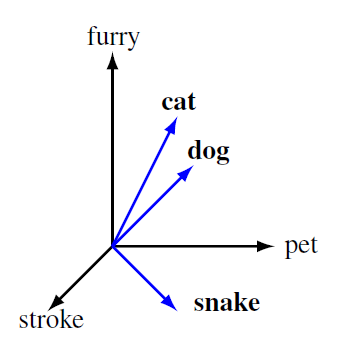
\includegraphics[width=\linewidth]{distributional.png}
 \end{aligned}$
 & $\begin{aligned}\mbox{{\color{blue} \huge +}}\end{aligned}$ & 
  $\begin{aligned}
 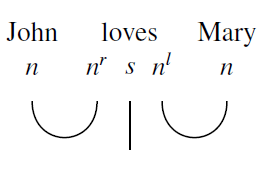
\includegraphics[width=\linewidth]{compositional.png}
 \end{aligned}$
\end{tabular}
\end{center}
\caption[The DisCo approach.]{The DisCo approach combines word vectors with pregroup or combinatory categorical grammar. The diagram on the right shows which terms cancel in the derivation tree.  It is drawn suggestively as explained in Section \ref{sec:disco}. }
\label{fig:discofig}
\end{figure}

In this model, each grammatical type is assigned a tensor product space based on Lambek's pregroup grammar \cite{lambek2008word} or combinatorial categorical grammar \cite{hermann2013role}. The meaning of nouns is, for example, calculated as in the distributional case, and we label their vector space $\mathcal{N}$.  A transitive verb's meaning is then, following the grammar, a vector in the space $\mathcal{N}\otimes \mathcal{S} \otimes \mathcal{N}$, where $\mathcal{S}$ is the meaning space for sentences \cite{clark2008compositional}. An intuition for this is that the transitive verb takes a subject noun as a left argument and an object noun as a right argument. An adjective lives in the space $\mathcal{N}\otimes\mathcal{N}$.

The oPT diagrammatic notation for vectors, tensors, and linear maps is commonly used in CCS. Here vertical composition (read bottom to top) represents composition of linear maps and horizontal composition represents the tensor product:
\begin{align*}
\begin{tabular}{cc}
\overrightarrow{\mbox{Mary}}\in \mathcal{N} :=
\begin{aligned}
\begin{tikzpicture}[scale=0.7, yscale=-1]
                \node  (20) at (0, 0) {$\mathcal{N}$};
                \node  (31) at (0, 2.5) {Mary};
                \node (1) [state] at (0,1) {};
                \draw  (0,0.5) to (1.center);
\end{tikzpicture}
\end{aligned} & \qquad
$f:\mathcal{M}\to\mathcal{N} :=$
\begin{aligned}
\begin{tikzpicture}[scale=0.7]
                \node  (20) at (0, -1.5) {$\mathcal{M}$};
                \node  (20) at (0, 1.5) {$\mathcal{N}$};                
                \node (1) [morphism] at (0,0) {f};
                \draw  (0,1) to (0,0.5);   
                \draw  (0,-1) to (0,-0.5);
\end{tikzpicture}
\end{aligned} \\
\overrightarrow{\mbox{likes}}\in \mathcal{N}\otimes\mathcal{S}\otimes \mathcal{N} :=
\begin{aligned}
\begin{tikzpicture}[scale=0.7,yscale=-1]
                \node  (3) at (-1, 1) {};
                \node  (4) at (2, 1) {};
                \node  (5) at (0.5, 2.25) {};
                \node  (10) at (-0.25, 1) {};
                \node  (11) at (0.5, 1) {};
                \node  (12) at (1.25, 1) {};
                \node  (15) at (-0.25, 0.5) {};
                \node  (16) at (0.5, 0.5) {};
                \node  (17) at (1.25, 0.5) {};
                \node  (20) at (-0.25, 0) {$\mathcal{N}$};
                \node  (21) at (0.5, 0) {$\mathcal{S}$};
                \node  (22) at (1.25, 0) {$\mathcal{N}$};
                \node  (31) at (0.5, 2.75) {likes};
                \draw  (3.center) to (4.center);
                \draw (4.center) to (5.center);
                \draw (3.center) to (5.center);
                \draw (10.center) to (15.center);
                \draw (11.center) to (16.center);
                \draw (12.center) to (17.center);
\end{tikzpicture}
\end{aligned} 
 & \qquad
 \begin{aligned}
 \begin{tikzpicture}[yscale=1.4]
                \node (0) at (0, 1) {};
                \node (2) at (-1, 0) {$g\circ f = $};
                \node (1) at (0.5, 1) {$\mathcal{P}$};
                \node (3) at (0, -1) {};
                \node [style=morphism] (4) at (0, -0.5) {$f$};
                \node (5) at (0.5, -1) {$\mathcal{M}$};
                \node (6) at (0.5, 0) {$\mathcal{N}$};
                \node [style=morphism] (7) at (0, 0.5) {$g$};
                \draw (3.center) to (0, -0.75);
                \draw (0, -0.25) to (0, 0.25);
                \draw (0, 0.75) to (0.center);
    \end{tikzpicture}
    \end{aligned} \\
\overrightarrow{\mbox{Mary}}\otimes \overrightarrow{\mbox{likes}} :=
\begin{aligned}
\begin{tikzpicture}[scale=0.7,yscale=-1]
                \node  (20) at (0, 0) {$\mathcal{N}$};
                \node  (31) at (0, 2.5) {Mary};
                \node (1) [state] at (0,1) {};
                \draw  (0,0.5) to (1.center);
                \node (2) [state, xscale=1.5, yscale=1] at (3,1) {};
                \node  (32) at (3, 2.5) {likes};
                \node  (20) at (2.25, 0) {$\mathcal{N}$};                                \node  (20) at (3, 0) {$\mathcal{S}$};
                \node  (20) at (3.75, 0) {$\mathcal{N}$};
                \draw  (3,0.5) to (2.center);
                \draw  (3.75,0.5) to (3.75,1);                            \draw  (2.25,0.5) to (2.25,1);    
\end{tikzpicture}
\end{aligned} & \qquad\qquad
\sum\limits_i \langle ii| :=
\begin{aligned}
\begin{tikzpicture}[scale=0.7, yscale=-1]
                \node  (0) at (-1, 1.5) {$\mathcal{N}$};
                \node  (1) at (1, 1.5) {$\mathcal{N}$};
                \node  (0) at (-1, 1) {};
                \node  (1) at (1, 1) {};
                \node  (2) at (0, 0) {};
                \draw [bend right=45, looseness=1.00] (0.center) to (2.center);
                \draw [bend right=45, looseness=1.00] (2.center) to (1.center);               
\end{tikzpicture}
\end{aligned}
\end{tabular}
\end{align*}
where $f:\mathcal{N}\to\mathcal{M}$ and $g:\mathcal{M}\to\mathcal{P}$ are linear maps and the linear map $\sum_i\langle ii|$ sums over all the basis vectors of $\mathcal{N}$ and is the usual oPT cap.

Given a well-typed sentence with meaning vectors $\vec{w_j}$ for each of $k$ words, the classical CCS algorithm for calculating a sentence's meaning is \cite{clark2013quantum}:
\begin{enumerate}
\item Compute the tensor product $\overrightarrow{\mbox{words}}=\vec{w_0}\otimes...\otimes \vec{w_k}$ in the order that each word appears in the sentence.

\item Construct a linear map that represents the type reduction by ``wiring up" the vectors with the appropriate caps as in the following example:

\begin{equation}
\label{eq:svo}
\begin{aligned}
\begin{tikzpicture}[scale=0.5, yscale=-1]
        \begin{pgfonlayer}{nodelayer}     
                \node (0) at (-3.5, 1) {};
                \node (1) at (-2, 1) {};
                \node (2) at (-2.75, 2) {};
                \node (3) at (-1, 1) {};
                \node (4) at (2, 1) {};
                \node (5) at (0.5, 2.25) {};
                \node (6) at (4.5, 1) {};
                \node (7) at (3.75, 2) {};
                \node (8) at (3, 1) {};
                \node (9) at (-2.75, 1) {};
                \node (10) at (-0.25, 1) {};
                \node (11) at (0.5, 1) {};
                \node (12) at (1.25, 1) {};
                \node (13) at (3.75, 1) {};
                \node (14) at (-2.75, 0.5) {};
                \node (15) at (-0.25, 0.5) {};
                \node (16) at (0.5, 0.5) {};
                \node (17) at (1.25, 0.5) {};
                \node (18) at (3.75, 0.5) {};
                \node (19) at (-2.75, 0) {$N$};
                \node (20) at (-0.25, 0) {$N$};
                \node (21) at (0.5, 0) {$S$};
                \node (22) at (1.25, 0) {$N$};
                \node (23) at (3.75, 0) {$N$};
                \node (24) at (-2.75, -0.5) {};
                \node (25) at (-0.25, -0.5) {};
                \node (26) at (0.5, -0.5) {};
                \node (27) at (1.25, -0.5) {};
                \node (28) at (3.75, -0.5) {};
                \node (29) at (0.5, -1.75) {};
                \node (30) at (-2.75, 2.75) {Mary};
                \node (31) at (0.5, 2.75) {likes};
                \node (32) at (3.75, 2.75) {words.};
        \end{pgfonlayer}
        \begin{pgfonlayer}{edgelayer}
                \draw (0.center) to (1.center);
                \draw (1.center) to (2.center);
                \draw (2.center) to (0.center);
                \draw  (3.center) to (4.center);
                \draw (8.center) to (6.center);
                \draw (6.center) to (7.center);
                \draw (4.center) to (5.center);
                \draw (3.center) to (5.center);
                \draw (8.center) to (7.center);
                \draw (9.center) to (14.center);
                \draw (10.center) to (15.center);
                \draw (11.center) to (16.center);
                \draw (12.center) to (17.center);
                \draw (13.center) to (18.center);
                \draw [thick, bend right=90, looseness=1.25] (24.center) to (25.center);
                \draw [thick, bend right=90, looseness=1.25] (27.center) to (28.center);
                \draw (26.center) to (29.center);
        \end{pgfonlayer}
\end{tikzpicture}
\end{aligned}
\end{equation}

\item Compute the meaning of the sentence by applying the linear map to the $\overrightarrow{\mbox{words}}$ vector. This results in a vector in $\mathcal{S}$ which corresponds to the meaning of the sentence.
\end{enumerate}

\noindent We refer the reader to \cite{coecke2010mathematical} for a fuller description of the distributional compositional model and to \cite{experimental-catcompdist} and \cite{kartsaklis2012unified} for experimental implementations.

These models suggest a promising approach to incorporate grammatical structure with vector space models of meaning, yet they come with the computational challenges of large tensor product spaces \cite{GrefenstetteThesis2013}. While there do exist some classical approaches to avoid the calculation of the full tensor product, such as the holographic reduced representations from \cite{plate1991holographic} or the use of dimensionality reduction \cite{polajnar2013learning}, these approaches introduce further assumptions and inaccuracies.  For this reason, ameliorating the large computational costs introduced these large spaces through quantum computation is of particular interest.

\section{Quantum computation for the CCS model}

The most immediate advantage for quantum implementations of the CCS model is gained by storing meaning vectors in quantum systems.  For $\alpha,\beta\in \mathbb{C}$ a two-level quantum system, a qubit, is defined by:
\begin{center}
  \begin{tabular}{cc}
   Qubit & Qubits  \\
   \begin{array}{lcl}
        \ket{\psi} &=& \alpha\ket{0}+\beta\ket{1} \\[0.2cm]
        &=&\alpha\left(\begin{array}{c} 1 \\ 0 \end{array}\right)
            +\beta\left(\begin{array}{c} 0 \\ 1 \end{array}\right)
   \end{array} 
   &\qquad\qquad
   \ket{\psi_1}\otimes\ket{\psi_2} = \left(\begin{array}{c} \alpha_1\alpha_2 \\ \alpha_1\beta_2\\\beta_1\alpha_2\\\beta_2\beta_2 \end{array}\right)
   \\
  \end{tabular}
\end{center}
and composition of qubits is given by the tensor product.  This leaves each $n$-qubit system with $2^n$ degrees of freedom, indicating that $N$-dimensional classical vectors can be stored in $\log_2 N$ qubits.
Consider a corpus whose word-meaning space is given by a basis of the 2,000 most common words. Even if we make the simplifying assumption that the sentence-meaning space is no larger than the word-meaning space we obtain the dramatic improvements details in Table 1.

\begin{table}[t]
\label{tab:space}
\begin{center}
\begin{tabular}{|c|c|c|}\hline
 & One Transitive Verb & 10k tr. verbs \\\hline
 Classical & $8\times 10^{9}$ bits & $8\times 10^{13}$ bits \\\hline
 Quantum & 33 qubits & 47 qubits \\\hline
\end{tabular}
\end{center}
\caption{Rough comparisons of the storage necessary for verbs in quantum and classical frameworks.}
\end{table}

Further, these word meanings can be imported into a ``bucket bridgade" quantum RAM that allows them to retrieved with a complexity linear in the number of qubits~\cite{giovannetti2008quantum}. The general point is that because quantum systems compose via the tensor product they are a natural choice to store complex types and sentences that have the same compositional structure. We can then employ quantum algorithms on for natural language classification as presented in Section \ref{sec:discoQalg}.

\section{A quantum algorithm for the closest vector problem}
\label{sec:qalg}

Many tasks in computational linguistics such as clustering, text classification, phrase/word similarity, and sentiment analysis rely on computations that determine the closest vector to $\vec{s}$ out of some set of $N$-dimensional vectors $\{\vec{v}_0,\vec{v}_1,...\vec{v}_{M-1}\}$. In clustering algorithms, for example, the set of vectors could be either the centroids of different clusters or the full set of training vectors, as in nearest neighbor clustering algorithms. Either the inner-product distance or Euclidean distance can be used. We will assume that all vectors are $N$-dimensional.
\begin{definition}
Given vector $\vec{s}$ and a set of $M$ vectors $U = \{\vec{v}_0,\vec{v}_1,...\vec{v}_{M-1}\}$ the \textbf{closest vector problem} asks one to determine which $v_j$ has the smallest inner product distance with $\vec{s}$.
\end{definition}
Direct calculation of the smallest vector would have complexity $\mathcal{O}(MN)$.  In \cite{wiebe2014quantum} the authors introduce a quantum algorithm for this problem that, under certain conditions, demonstrate quadratic speedups over direct calculation and polynomial speedups over Monte-Carlo methods. Some proof of principle experiments have then demonstrated clustering of eight-dimensional vectors, based on these techniques, on a small photonic quantum computer \cite{cai2015entanglement}. This algorithm requires the following assumptions, where we write $v_{ji}$ for the $i$^{\tiny\mbox{th}}$ entry of the $j$^{\tiny\mbox{th}}$ vector:
\begin{enumerate}
\item Vectors $\vec{v_j}$ and $\vec{s}$ are $d$-sparse, with no more than $d$ non-zero entries.
\item The relevant vectors are stored in some kind of quantum memory so that the quantum computer can access their entries with the two oracles of the form:
\begin{equation}
\begin{array}{c}
\mathcal{O}\ket{j}\ket{i}\ket{0}:=\ket{j}\ket{i}\ket{v_{ji}}, \\
\mathcal{F}\ket{j}\ket{l}:= \ket{j}\ket{f(j,l)},
\end{array}
\end{equation}
where $f(j,l)$ is the location of the $l$^{\tiny\mbox{th}}$ non-zero entry of $v_j$.  It is against these memory access oracles that the performance of our algorithm will be measured.

\item $\max(|v_{ji}|^2)\le r_{\small\mbox{max}}$ for some known constant $r_{\small\mbox{max}}$.

\item All the vectors are normalized.
 
\end{enumerate}

Under these assumptions we are able to run a quantum nearest-neighbor algorithm with complexity characterized by the following theorem:

\begin{theorem}[\cite{wiebe2014quantum}]
We can find $\max_j|\langle s~|~v_j\rangle|^2$ with success probability $1-\delta$ and error $\epsilon$ using an expected number of $\mathcal{O}$ and $\mathcal{F}$ queries that is bounded above by
\begin{equation}
1080\sqrt{M}\left\lceil\frac{4\pi(\pi+1)d^2r^4_{\tiny\mbox{max}}}{\epsilon}\right\rceil\left\lceil \frac{\ln\left(81M(\ln(M)+\gamma)\right)/\delta_0}{2(8/\pi^2-1/2)^2}\right\rceil,
\end{equation}
where $\gamma\approx 0.5772$ is Euler's constant.
\end{theorem}

It is clear that for this quantum algorithm there is a quadratic improvement in scaling with $M$, the number of training vectors. While the dimension of the vectors $N$ is not explicitly included, in general it is implicitly there through the dependence on $d$.  It is also clear that if $r_{\small\mbox{max}}\propto 1/\sqrt{d}$, then the algorithm's dependence on both $d$ and $N$ drops out. As the vectors are normalized, this can be expected to occur if the vectors have sparsity that grows linearly with their size \cite{wiebe2014quantum}. The authors further assume that for ``typical" cases the error $\epsilon$ scales as $\Theta(1/\sqrt{N})$ so that the runtime for the quantum inner-product algorithm becomes $\mathcal{O}\left(\sqrt{NM}\ln(M)d^2r^4_{\small\mbox{max}}\right)$.\footnote{
This is argued for in Appendix D of \cite{wiebe2014quantum} for a ``typical" case where the vectors are uniformly distributed over the unit sphere.} This result shows a quadratic improvement over direct calculations and also shows improvement over Monte Carlo methods, whose complexity is $\mathcal{O}\left(NMd^2r^4_{\small\mbox{max}}\right)$. These comparisons are summarized in Table 2.

\begin{table}[ht]
\label{tab:comp}
\begin{center}
\begin{tabular}{|c|c|c|}\hline
 Type & Typical cases & Atypical cases    \\ \hline
 Classical Direct & $\mathcal{O}(NM)$ & $\mathcal{O}(NM)$ \\
 Classical Monte Carlo & $\mathcal{O}\left(NMd^2r_{\small\mbox{max}}^4\right)$ & $\mathcal{O}\left(Md^2r_{\small\mbox{max}}^4/\epsilon^2\right)$ \\
 Quantum & $\mathcal{O}\left(\sqrt{NM}\log(M)d^2r^4_{\small\mbox{max}}\right)$ &  $\mathcal{O}\left(\sqrt{M}\log(M)d^2r^4_{\small\mbox{max}}/\epsilon\right)$ \\\hline
\end{tabular}
\end{center}
\caption{Complexity comparisons for different closest vector algorithms. Adapted from \cite{wiebe2014quantum}.}
\end{table}

 In the following section we adapt this algorithm to sentence similarity calculations in the distributional compositional framework.

\section{A quantum algorithm for CCS sentence similarity}
\label{sec:discoQalg}

The quantum algorithm from Section \ref{sec:qalg} can be used to advantage in natural language processing tasks however, the computational overhead of the CCS approach would dwarf this algorithm's advantages if it were naively applied.  
Throughout this section we will assume both that $r_{\small\mbox{max}}\propto 1/\sqrt{d}$ and that the accuracy necessary for our calculation means $\epsilon$ scales as $\Theta(1/\sqrt{N})$. Consider the example of probabilistically classifying the meaning of a  simple sentence. We illustrate this example with a noun-verb-noun sentence. The meaning of the nouns are vectors in an $N$-dimensional vector space and the meaning of the verb is a vector in the space $N\otimes S \otimes N$. We represent a derivation of the meaning of the full sentence with the following map:

\begin{equation}
\label{eqn:phi}
\begin{aligned}
\begin{tikzpicture}[scale=0.6, yscale=-1]
        \begin{pgfonlayer}{nodelayer}
                \node (0) at (-5.5, 0) {\ket{\phi}};
                \node (0) at (-4.5, 0) {=};       
                \node (0) at (-3.5, 1) {};
                \node (1) at (-2, 1) {};
                \node (2) at (-2.75, 2) {};
                \node (3) at (-1, 1) {};
                \node (4) at (2, 1) {};
                \node (5) at (0.5, 2.25) {};
                \node (6) at (4.5, 1) {};
                \node (7) at (3.75, 2) {};
                \node (8) at (3, 1) {};
                \node (9) at (-2.75, 1) {};
                \node (10) at (-0.25, 1) {};
                \node (11) at (0.5, 1) {};
                \node (12) at (1.25, 1) {};
                \node (13) at (3.75, 1) {};
                \node (14) at (-2.75, 0.5) {};
                \node (15) at (-0.25, 0.5) {};
                \node (16) at (0.5, 0.5) {};
                \node (17) at (1.25, 0.5) {};
                \node (18) at (3.75, 0.5) {};
                \node (19) at (-2.75, 0) {$N$};
                \node (20) at (-0.25, 0) {$N$};
                \node (21) at (0.5, 0) {$S$};
                \node (22) at (1.25, 0) {$N$};
                \node (23) at (3.75, 0) {$N$};
                \node (24) at (-2.75, -0.5) {};
                \node (25) at (-0.25, -0.5) {};
                \node (26) at (0.5, -0.5) {};
                \node (27) at (1.25, -0.5) {};
                \node (28) at (3.75, -0.5) {};
                \node (29) at (0.5, -1.75) {};
                \node (30) at (-2.75, 2.75) {kids};
                \node (31) at (0.5, 2.75) {play};
                \node (32) at (3.75, 2.75) {football};
        \end{pgfonlayer}
        \begin{pgfonlayer}{edgelayer}
                \draw (0.center) to (1.center);
                \draw (1.center) to (2.center);
                \draw (2.center) to (0.center);
                \draw  (3.center) to (4.center);
                \draw (8.center) to (6.center);
                \draw (6.center) to (7.center);
                \draw (4.center) to (5.center);
                \draw (3.center) to (5.center);
                \draw (8.center) to (7.center);
                \draw (9.center) to (14.center);
                \draw (10.center) to (15.center);
                \draw (11.center) to (16.center);
                \draw (12.center) to (17.center);
                \draw (13.center) to (18.center);
                \draw [thick, bend right=90, looseness=1.25] (24.center) to (25.center);
                \draw [thick, bend right=90, looseness=1.25] (27.center) to (28.center);
                \draw (26.center) to (29.center);
        \end{pgfonlayer}
\end{tikzpicture}
\end{aligned}
\end{equation}

From now on, we will take sentences to exist in the same meaning space as words, i.e. $S\simeq N$.

\begin{definition}
For meaning vector $\vec{s}$ and $M$ sets of meaning vectors, a \textbf{classification task} assigns $\vec{s}$ to the set containing the nearest-neighbor of $\vec{s}$.
\end{definition}

An example task would be to determine if a sentence is about sports or politics or if a sentence expresses agreement or disagreement. 
%The \textbf{classification} approach considers the closest set to be given %by the set whose average vector has the smallest inner product with $s$. %We define these average vectors as 
%\begin{align*}
%v &= \frac{1}{m}\sum_m v_i \qquad \qquad
%w = \frac{1}{m}\sum_m w_i.
%\end{align}
%In the simplest case, there is only a single meaning vector in each training %cluster, i.e. $m=1$. 
If, to present a simplified example, we take each cluster to only contain a single vector ($\vec{v}$ and $\vec{w}$ respectively) then the sentence would be classified by computing 
\begin{equation}
\label{eq:exampleCalcs}
\begin{aligned}
\begin{tikzpicture}[scale=0.5, yscale=-1]
        \begin{pgfonlayer}{nodelayer}
                \node (0) at (-3.5, 1) {};
                \node (1) at (-2, 1) {};
                \node (2) at (-2.75, 2) {};
                \node (3) at (-1, 1) {};
                \node (4) at (2, 1) {};
                \node (5) at (0.5, 2.25) {};
                \node (6) at (4.5, 1) {};
                \node (7) at (3.75, 2) {};
                \node (8) at (3, 1) {};
                \node (9) at (-2.75, 1) {};
                \node (10) at (-0.25, 1) {};
                \node (11) at (0.5, 1) {};
                \node (12) at (1.25, 1) {};
                \node (13) at (3.75, 1) {};
                \node (14) at (-2.75, 0.5) {};
                \node (15) at (-0.25, 0.5) {};
                \node (16) at (0.5, 0.5) {};
                \node (17) at (1.25, 0.5) {};
                \node (18) at (3.75, 0.5) {};
                \node (19) at (-2.75, 0) {$N$};
                \node (20) at (-0.25, 0) {$N$};
                \node (21) at (0.5, 0) {$S$};
                \node (22) at (1.25, 0) {$N$};
                \node (23) at (3.75, 0) {$N$};
                \node (24) at (-2.75, -0.5) {};
                \node (25) at (-0.25, -0.5) {};
                \node (26) at (0.5, -0.5) {};
                \node (27) at (1.25, -0.5) {};
                \node (28) at (3.75, -0.5) {};
                \node (29) at (0.5, -1.75) {};
                \node (30) at (-2.75, 2.75) {kids};
                \node (31) at (0.5, 2.75) {play};
                \node (32) at (3.75, 2.75) {football};
                \node [style=state, hflip] (33) at (0.5, -1.75) {$\vec{v}$};
                \node (34) at (0.6, -3.5) {sports};
        \end{pgfonlayer}
        \begin{pgfonlayer}{edgelayer}
                \draw (0.center) to (1.center);
                \draw (1.center) to (2.center);
                \draw (2.center) to (0.center);
                \draw  (3.center) to (4.center);
                \draw (8.center) to (6.center);
                \draw (6.center) to (7.center);
                \draw (4.center) to (5.center);
                \draw (3.center) to (5.center);
                \draw (8.center) to (7.center);
                \draw (9.center) to (14.center);
                \draw (10.center) to (15.center);
                \draw (11.center) to (16.center);
                \draw (12.center) to (17.center);
                \draw (13.center) to (18.center);
                \draw [thick, bend right=90, looseness=1.25] (24.center) to (25.center);
                \draw [thick, bend right=90, looseness=1.25] (27.center) to (28.center);
                \draw (26.center) to (29.center);
        \end{pgfonlayer}
\end{tikzpicture}
\end{aligned}
&& \qquad \mbox{and}} \qquad
\begin{aligned}
\begin{tikzpicture}[scale=0.5, yscale=-1]
        \begin{pgfonlayer}{nodelayer}
                \node (0) at (-3.5, 1) {};
                \node (1) at (-2, 1) {};
                \node (2) at (-2.75, 2) {};
                \node (3) at (-1, 1) {};
                \node (4) at (2, 1) {};
                \node (5) at (0.5, 2.25) {};
                \node (6) at (4.5, 1) {};
                \node (7) at (3.75, 2) {};
                \node (8) at (3, 1) {};
                \node (9) at (-2.75, 1) {};
                \node (10) at (-0.25, 1) {};
                \node (11) at (0.5, 1) {};
                \node (12) at (1.25, 1) {};
                \node (13) at (3.75, 1) {};
                \node (14) at (-2.75, 0.5) {};
                \node (15) at (-0.25, 0.5) {};
                \node (16) at (0.5, 0.5) {};
                \node (17) at (1.25, 0.5) {};
                \node (18) at (3.75, 0.5) {};
                \node (19) at (-2.75, 0) {$N$};
                \node (20) at (-0.25, 0) {$N$};
                \node (21) at (0.5, 0) {$S$};
                \node (22) at (1.25, 0) {$N$};
                \node (23) at (3.75, 0) {$N$};
                \node (24) at (-2.75, -0.5) {};
                \node (25) at (-0.25, -0.5) {};
                \node (26) at (0.5, -0.5) {};
                \node (27) at (1.25, -0.5) {};
                \node (28) at (3.75, -0.5) {};
                \node (29) at (0.5, -1.75) {};
                \node (30) at (-2.75, 2.75) {kids};
                \node (31) at (0.5, 2.75) {play};
                \node (32) at (3.75, 2.75) {football};
                \node [style=state, hflip] (33) at (0.5, -1.75) {$\vec{w}$};
                \node (34) at (0.6, -3.5) {politics};
        \end{pgfonlayer}
        \begin{pgfonlayer}{edgelayer}
                \draw (0.center) to (1.center);
                \draw (1.center) to (2.center);
                \draw (2.center) to (0.center);
                \draw  (3.center) to (4.center);
                \draw (8.center) to (6.center);
                \draw (6.center) to (7.center);
                \draw (4.center) to (5.center);
                \draw (3.center) to (5.center);
                \draw (8.center) to (7.center);
                \draw (9.center) to (14.center);
                \draw (10.center) to (15.center);
                \draw (11.center) to (16.center);
                \draw (12.center) to (17.center);
                \draw (13.center) to (18.center);
                \draw [thick, bend right=90, looseness=1.25] (24.center) to (25.center);
                \draw [thick, bend right=90, looseness=1.25] (27.center) to (28.center);
                \draw (26.center) to (29.center);
        \end{pgfonlayer}
\end{tikzpicture}
\end{aligned}
\end{equation}
and assigning the sentence to the one of smaller value.  We would proceed with two steps:

\begin{enumerate}
\item Compute the derivation of $\ket{\phi}$, which, by classical direct calculation, takes  $\mathcal{O}(3N)$ operations. 

\item See which of $\vec{v}$ and $\vec{w}$ is closest to $\ket{\phi}$. This is an instance of the closest vector problem where $\vec{s} = \ket{\phi}$, $M=2$, and $U = \{\vec{v},\vec{w}\}$. With direct calculation or Monte Carlo the second step requires\footnote{If we assume the appropriate $d$-sparsity scaling.} $\mathcal{O}(2N)$ to be compared with the quantum method at $\mathcal{O}(\sqrt{2N}\log 2)$. Even if we include the step to import the classical data from step one into quantum form, which can be done with $\mathcal{O}(\log_2N)$ overhead \cite{giovannetti2008quantum}, then we obtain a speedup for this step. 
\end{enumerate}

Still, despite the quantum speedup from step two, the full algorithm for general $M$ runs in $\mathcal{O}(3N\sqrt{M}\log M)$, remaining linear in $N$.

In order to recover a speedup we refine the application of the quantum algorithm by posing a version of the closest vector problem that avoids the initial calculation of $\ket{\phi}$ altogether. Note the equivalence of the calculations in Equation \ref{eq:exampleCalcs} with 
\begin{equation}
\label{eqn:trick}
\begin{aligned}
\begin{tikzpicture}[scale=0.5, yscale=-1]
        \begin{pgfonlayer}{nodelayer}
                \node (3) at (-3, 1) {};
                \node (4) at (4, 1) {};
                \node (5) at (0.5, 2.25) {};
                \node (10) at (-2, 1) {};
                \node (11) at (0.5, 1) {};
                \node (12) at (3, 1) {};
                \node (13) at (3.75, 1) {};
                \node (14) at (-2.75, 0.5) {};
                \node (15) at (-2, 0.5) {};
                \node (16) at (0.5, 0.5) {};
                \node (17) at (3, 0.5) {};
                \node (18) at (3.75, 0.5) {};
                \node (20) at (-2, 0) {$N$};
                \node (21) at (0.5, 0) {$S$};
                \node (22) at (3, 0) {$N$};
                \node (24) at (-2.75, -0.5) {};
                \node (25) at (-0.25, -0.5) {};
                \node (26) at (0.5, -0.5) {};
                \node (27) at (1.25, -0.5) {};
                \node (28) at (3.75, -0.5) {};
                \node (29) at (0.5, -1.75) {};
                \node (30) at (-2, -3.5) {kids};
                \node (31) at (0.5, 2.75) {play};
                \node (32) at (3.5, -3.5) {football};
                \node [style=state, hflip] (33) at (-2, -1.75) {};
                \node [style=state, hflip] (35) at (0.5, -1.75) {};
                \node [style=state, hflip] (36) at (3, -1.75) {};
                \node (34) at (0.6, -3.5) {sports};
        \end{pgfonlayer}
        \begin{pgfonlayer}{edgelayer}
                \draw  (3.center) to (4.center);
                \draw (4.center) to (5.center);
                \draw (3.center) to (5.center);
                \draw (10.center) to (15.center);
                \draw (11.center) to (16.center);
                \draw (12.center) to (17.center);
                \draw (26.center) to (29.center);
                \draw (-2,-0.5) to (33.center);
                \draw (3,-0.5) to (36.center);
        \end{pgfonlayer}
\end{tikzpicture}
\end{aligned}
&& \qquad \mbox{and}} \qquad
\begin{aligned}
\begin{tikzpicture}[scale=0.5, yscale=-1]
        \begin{pgfonlayer}{nodelayer}
                \node (3) at (-3, 1) {};
                \node (4) at (4, 1) {};
                \node (5) at (0.5, 2.25) {};
                \node (10) at (-2, 1) {};
                \node (11) at (0.5, 1) {};
                \node (12) at (3, 1) {};
                \node (13) at (3.75, 1) {};
                \node (14) at (-2.75, 0.5) {};
                \node (15) at (-2, 0.5) {};
                \node (16) at (0.5, 0.5) {};
                \node (17) at (3, 0.5) {};
                \node (18) at (3.75, 0.5) {};
                \node (20) at (-2, 0) {$N$};
                \node (21) at (0.5, 0) {$S$};
                \node (22) at (3, 0) {$N$};
                \node (24) at (-2.75, -0.5) {};
                \node (25) at (-0.25, -0.5) {};
                \node (26) at (0.5, -0.5) {};
                \node (27) at (1.25, -0.5) {};
                \node (28) at (3.75, -0.5) {};
                \node (29) at (0.5, -1.75) {};
                \node (30) at (-2, -3.5) {kids};
                \node (31) at (0.5, 2.75) {play};
                \node (32) at (3.5, -3.43) {football};
                \node [style=state, hflip] (33) at (-2, -1.75) {};
                \node [style=state, hflip] (35) at (0.5, -1.75) {};
                \node [style=state, hflip] (36) at (3, -1.75) {};
                \node (34) at (0.6, -3.54) {politics};
        \end{pgfonlayer}
        \begin{pgfonlayer}{edgelayer}
                \draw (3.center) to (4.center);
                \draw (4.center) to (5.center);
                \draw (3.center) to (5.center);
                \draw (10.center) to (15.center);
                \draw (11.center) to (16.center);
                \draw (12.center) to (17.center);
                \draw (26.center) to (29.center);
                \draw (-2,-0.5) to (33.center);
                \draw (3,-0.5) to (36.center);
        \end{pgfonlayer}
\end{tikzpicture}
\end{aligned}
\end{equation}
Rather than directly calculating $\ket{\phi}$, which is not relevant to the classification task, we can formulate a closest vector problem where $\vec{s} = \ket{play}$, $M=2$ and $U = \{\ket{kids}\otimes\ket{v} \otimes\ket{football},\ket{kids}\otimes\ket{w} \otimes\ket{football}\}$.
The runtime of this \textbf{deferred quantum algorithm}, including import, will then be $\mathcal{O}(\sqrt{MN})$, showing our desired quadratic speedup in both variable.

We extend this to result to include general sentences in the CCS model with the following theorem.\footnote{The authors would like to thank an anonymous reviewer for correcting an error in the original statement of the algorithm.}

\begin{theorem}
For an $N$-dimensional noun meaning space, there exists a quantum algorithm to classify any CCS model sentence composed of $n$ tensors $\vec{w_0},\vec{w_1},...,\vec{w_{n-1}}$ whose maximum dimension is $N^k$ into $M$ classes with time $\mathcal{O}(\sqrt{M N^{k(n-1)/2}} \log M)$. This is not always an improvement on the classical algorithm which runs in $\mathcal{O}(MN)$, but will be if $k(n-1) < 4$ (very short sentence fragments) or if $M$ is much larger than $N$, thought this lasts case is unlikely in practice.
\end{theorem}
\begin{proof}
The trick we play in Equation \ref{eqn:trick} amounts to splitting the sentence derivation into a bipartite graph.  As the CCS connections are based on a pregroup derivation, the connections will always form a tree, taking words as nodes and connections as edges. Trees can always be partitioned into bipartite graphs, thus, up to the ordering of inputs on each tensor which can be kept track of, we can always give a deferred quantum algorithm with associated speedup for any such CCS sentence.
 The following procedure explicitly details how to construct this bipartite partitioning.

For every CCS sentence there is one word that acts as the \textbf{head} of the derivation.  This is the word whose output $S$ wire contains the sentence meaning following its derivation's linear map. In Equation \ref{eqn:phi} this is the word ``play". Connect the dangling wire of the head word $\vec{w_h}$ with the vector $\vec{v_i}$ against which similarity is being measured.  Starting with this head word we then separate the sentence into a top layer and a bottom layer with the following steps.  Assign the head word to the top layer. Place every word it is connected to on the bottom layer. Next for every word just assigned to the bottom, take all their connected words, which are not yet assigned, and assign them to the top.  Continue this procedure while alternating top and bottom until all words are assigned. This gives a simple two-coloring of the derivation graph. 
\end{proof}

\begin{example}
Consider the following example sentence from \cite{dimitriThesis}:
\begin{equation*}
\begin{tikzpicture}[scale=1, yscale=-1]
                \node [style=state] (0) at (-6, 1) {1};
                \node (1) at (-5.25, 0.25) {};
                \node [style=state] (2) at (-2, 1) {2};
                \node [style=state] (3) at (2, 1) {2};
                \node [style=state] (4) at (3.5, 1) {3};
                \node (5) at (-1.25, 0.25) {};
                \node (6) at (1.25, 0.25) {};
                \node (7) at (2.75, 0.25) {};
                \node (8) at (-4.5, 1) {};
                \node (9) at (-3.5, 1) {};
                \node (10) at (-0.5, 1) {};
                \node (11) at (0.5, 1) {};
                \node (label1) at (0, 1.175) {1};
                \node [style=state, xscale=2] (12) at (0, 1) {};
                \node (label1) at (-4, 1.175) {0};
                \node [style=state, xscale=2] (13) at (-4, 1) {};
                \node (14) at (-4, -1) {};
                \node (15) at (-1.75, -0.5) {};
                \node (16) at (-6, 1.9) {John};
                \node (17) at (-4, 1.9) {saw};
                \node (18) at (-2, 1.9) {Mary};
                \node (19) at (0, 1.9) {read};
                \node (20) at (2, 1.9) {a};
                \node (21) at (3.5, 1.9) {book};
                \draw [bend right=45, looseness=1.00] (0) to (1.center);
                \draw [bend right=45, looseness=1.00] (2) to (5.center);
                \draw [in=-90, out=0, looseness=1.00] (7.center) to (4);
                \draw [bend left=45, looseness=1.00] (8.center) to (1.center);
                \draw (13) to (14.center);
                \draw [bend left=45, looseness=1.00] (10.center) to (5.center);
                \draw [bend right=45, looseness=1.00] (9.center) to (15.center);
                \draw [bend right=45, looseness=1.00] (11.center) to (6.center);
                \draw [bend right=45, looseness=1.00] (6.center) to (1.9,1);
                \draw [bend right=45, looseness=1.00] (2.1,1) to (7.center);
                \draw [bend right=45, looseness=1.00] (15.center) to (12);
\end{tikzpicture}
\end{equation}
where we have labeled the vectors based on their depth in the derivation tree.  The two-layer form assigns even vectors to the top layer and odd vectors to the bottom:
\begin{equation*}
\begin{tikzpicture}[scale=1, yscale=-1]
                \node [style=state, hflip] (0) at (-5, 0) {};
                \node [style=state] (1) at (-2.5, 1) {};
                \node [style=state] (2) at (-1.25, 1) {};
                \node [style=state, hflip] (3) at (-0.75, 0) {};
                \node (4) at (-4.5, 1) {};
                \node (5) at (-3.5, 1) {};
                \node (6) at (-2.5, -1) {};
                \node (7) at (-2, 0) {};
                \node [style=state, hflip, xscale=2] (8) at (-2.5, 0) {};
                \node [style=state, xscale=2] (9) at (-4, 1) {};
                \node (10) at (-4, -1) {};
                \node (11) at (-5, -0.75) {John};
                \node (12) at (-4, 1.75) {saw};
                \node (13) at (-2.5, 1.75) {Mary};
                \node (14) at (-2.5, -0.75) {read};
                \node (15) at (-1.25, 1.75) {a};
                \node (16) at (-0.75, -0.75) {book};
                \draw (9) to (10.center);
                \draw (4.center) to (0);
                \draw (1) to (-2.5,0);
                \draw (7.center) to (-1.4,1);
                \draw (-1,1) to (3);
                \draw (5.center) to (-3,0);
\end{tikzpicture}
\end{equation*}
\end{example}

\noindent Hooking the dangling wire up to a classifying vector reduces the similarity computation to the calculation of a single inner product. Note that this procedure works for any derivation tree,\footnote{Even non-pregroup and non-CCG models will work as long as there is some tree derivation.} so sentence fragments, such as noun phrases, can be easily analyzed in exactly the same manner. 

It is also very likely that other algorithms can be found, which decompose the sentence in other ways, and that give other time complexities.

\section{Noise tolerance and Conclusion}

To reap the benefits of quantum algorithm in the domain of natural language processing, we  apply a new technique to defer the calculation of a sentence's compositional meaning, eliminating the overhead costs. By this method we are able to introduce a quantum algorithm for calculating sentence similarity that offers quadratic speedup over classical direct calculation and Monte-Carlo methods. These kinds of algorithms are particularly attractive for practical applications of quantum computing as noisy results can be tolerated: in our case when the desired errors is lower bounded by $1/\sqrt{N}$.  Vector space models are already inherently noisy and typical tasks allow for errors in results, so this restriction does not affect their efficacy. 

An additional point is that the density matrix formalism of \cite{piedeleu2015open} can also be naturally modeled by mixed states of quantum systems.  In fact, this analogy was the genesis for the theory of disambiguation presented there, as another example of the shared structure that led to the results presented here. At a basic level, our work exploits the abstract connection between natural language processing and quantum information.  More formally,  we can see both quantum computation in the category of finite dimensional Hilbert spaces and linear maps \cite{abramsky2004categorical,cqm-notes} and CCS in the product category of pregroup grammar and finite dimensional vectors spaces \cite{coecke2010mathematical}. The connection between these two (as process theories) makes the application of one to the other apparent.

%\section{Models of quantum algorithms in sets and relations}
\label{sec:qalgrel}

        In this section, we construct abstract models of blackbox quantum algorithms using a model of quantum computation in sets and relations, a setting that is usually considered for nondeterministic classical computation.  This alternative model of quantum computation (QCRel), though unphysical, nevertheless faithfully models its computational structure.  Our main results are models of the Deutsch-Jozsa, single-shot Grover's, and GroupHomID algorithms in QCRel. These results provide new tools to analyze the semantics of quantum computation and improve our understanding of the relationship between computational speedups and the structure of physical theories. They also exemplify a method of extending physical/computational intuition into new mathematical settings.

\subsection{Introduction}

Having grasped the abstract structure at play in the protocols and algorithms of quantum computation, we can conceive of modelling quantum computation in oGCTs other than Hilbert spaces and linear maps.  There are two main thrusts that make this investigation, interesting.  The first is to further analyze the structure of quantum computation, advancing our understanding of the relationship between computational speedups and the structure of physical theories. We use the QCRel model defined here to analyze some example quantum algorithms as non-deterministic classical algorithms while preserving their query-complexity (and, in fact, all their abstract structure). The second thrust regards the insights that become available by extending physical/computational intuition into new areas of mathematics. While other toy models of a relational flavor for quantum mechanics have been proposed \cite{ellermanModelQM,discreteQT,modalQT,spekk}, and some even discuss protocols \cite{QCFF_James}, these works have not developed the structures necessary to model quantum algorithms.

First we construct our chosen model of quantum information.  This is the oGCT in \cat{FRel}, rather than \cat{FHilb}, and it is introduced by rephrasing the axioms of quantum mechanics. Next we present the novel contributions in this thesis: relational models of unitary oracles, the Deutsch-Jozsa algorithm, the single-shot Grover's algorithm, and the group homomorphism identification algorithm.

\subsection{The model of quantum computation in relations}
\label{sec:modelqcrel}
We begin with definitions of the key components of quantum computation in this new setting, e.g. systems, states, bases, observables, etc.  The following definitions are motivated by Chapter~\ref{chap:cqm}, whose general theorems prove useful. To avoid distracting repetition of notation, we use generic terminology to refer to the relational setting within this section.  For example \textbf{system} is intended to mean \textbf{relational system}, i.e. a set.  When we wish to refer to the quantum setting we explicitly denote this e.g. \textbf{quantum system} refers to a finite dimensional Hilbert space.

\begin{axiom}
A \textbf{system} is a set $H$ with \textbf{states} $|\psi\rangle$ given by subsets $\psi\subseteq H$.
\end{axiom}


\noindent Each state in our notation is a boolean column vector written as a labelled ket, to follow the convention in quantum mechanics where states are complex valued column vectors as in the following example. 
\begin{example}
\label{ex:columnvect}
Consider a three element system $\{0,1,2\}$, the relation $R=\{(0,0),(0,2),(1,1)\}$ and the state $\ket{\psi}=\{0\}$. In terms of boolean matrices and vectors the composition $R\circ\ket{\psi}$ is written as:
\begin{equation}
\left(\begin{array}{ccc}
1 & 0 & 0 \\
0 & 1 & 0 \\
1 & 0 & 0 \\
\end{array}\right)
\left(\begin{array}{c}
1 \\
0 \\
0 \\
\end{array}\right)
=
\left(\begin{array}{c}
1 \\
0 \\
1 \\
\end{array}\right).
\end{equation}
\end{example}
The state $|\psi\vee\phi\rangle$ has elements in the union of sets $\psi$ and $\phi$. We often use $\ket{\psi}$ to mean the relation $\{\star\}\to H$ that relates the singleton set to all the elements in $\psi$.

\begin{axiom}
A \textbf{composite system} $H$ of $n$ subsystems is given by the Cartesian product so that $H = H_1\times...\times H_n$. \textbf{Composite states} are any subset of $H$.
\end{axiom}

\begin{defn}
For a relation $R:A\to B$ from set $A$ to $B$, the \textbf{converse relation} is denoted $R^{-1}:B\to A$ where for $x\in A$ and $y\in B$, $xRy$ if and only if $yR^{-1}x$.
\end{defn}

\noindent The converse replaces the $\dagger$-adjoint in quantum mechanics. This leads to:

\begin{defn}
A relation $R:H_1\to H_2$ is \textbf{unitary} if and only if $R\circ R^{-1} = \mbox{id}_{H_1}$ and $R^{-1}\circ R = \mbox{id}_{H_2}$, where $Q\circ R$ means $Q$ after $R$.
\end{defn}

\noindent This is the relational analog to the usual unitarity of linear maps in quantum mechanics and has an obvious interpretation:

\begin{corollary}
\label{cor:bijections}
Relations are unitary if and only if they are bijections.
\end{corollary}

\begin{axiom}
\textbf{Evolution} of systems is given by unitary relations.
\end{axiom}

\noindent This means that states of system $A$ can evolve to states of system $B$ if and only if there is a bijection between them. Note that this implies that there do not exist physical evolutions between systems of different cardinality. %This is analogous to the quantum setting where there do not exist unitary %maps between Hilbert spaces of differing dimensions.

\begin{defn}
For a state $\ket{\psi}:\{\star\}\to H$, denote its relational converse as $\bra{\psi}:H\to\{\star\}$ called its \textbf{effect}.
\end{defn}

\noindent A state preparation followed by an effect amounts to an experiment with a post-selected outcome. Effects are maps to $\{\star\}$ that return whether the outcome state $\ket{\psi}$ is possible.
 We give an example to illustrate:
\begin{example}
The preparation of the state $\ket{\phi}$ followed by a post-selected measurement of the effect $\bra{\psi}$ is given by the relation
\begin{align*}
\langle\psi|\phi\rangle:=\bra{\psi}\circ\ket{\phi}:\{\star\}\to H\to \{\star\}
\end{align*}
This is either the identity relation that we interpret to mean a measurement outcome of $\bra{\psi}$ is \emph{possible}, or it is the empty relation that we interpret to mean the measurement outcome $\bra{\psi}$ is \emph{impossible}. It is clear that the outcome $\bra{\psi}$ is possible if there exists some element of $H$ in both $\psi$ and $\phi$. Otherwise it is impossible.
In this sense our relational quantum computation is a deterministic model of quantum computation.
\end{example}

This interpretation allows us to define a generalized version of the Born rule\footnote{In quantum theory, the Born rule gives the probability of measuring the outcome state $\ket{\psi}$ following preparation in state $\ket{\phi}$ as $|\langle\psi|\phi\rangle|^2$ where $\langle\psi|\phi\rangle:\mathbb{C}\to\mathbb{C}$ is the inner product of the two state vectors \cite{nielsen2010quantum}. The oGCT generalization is given in\ Definition~\ref{def:bornrule}.} to describe measurement in our model.
\begin{axiom}[Relational Born Rule]
\label{ax:relborn}
The possibility of measuring the state $\ket{\psi}$, having prepared state $\ket{\phi}$, is given by the image of:
\begin{align}
\langle\psi|\phi\rangle:\{\star\}\to\{\star\}
\end{align}
\end{axiom}

In the relational model, bases are characterized as particular generalizations of groups known as \textit{groupoids} \cite{cqm-notes,pavlovic2009quantum}.  Groupoids can be viewed as groups where multiplication is relaxed to be a partial function.

\begin{defn}
\label{def:basis}
For a system $H$, a \textbf{basis} $Z$ is a direct sum (disjoint union) of abelian groups $Z = G_0\oplus G_1\oplus...$ where $|Z| = |H|$.
Multiplication with respect to this list of groups will be written as $\bullet_Z$ and is defined in the following way. For elements $x,y\in Z$ such that $x\in G_i$ and $y\in G_j$ we have the partial function:
\begin{align}
\label{eq:groupoid_mult}
x\bullet_Zy = \begin{cases}
x +_{G_i} y & i=j \\
\mbox{undefined} & \mbox{otherwise}\\
\end{cases}
\end{align}
\noindent This makes $Z$ an \textbf{abelian groupoid} with groupoid multiplication $\bullet_Z$.
\end{defn}
We will sometimes take a categorical perspective on groupoids. A groupoid $Z=\bigoplus^NG_i$ made up $N$ groups is a category whose set of objects is isomorphic to the set of groups $\{G_i\}$ and whose morphisms are elements of $Z$, e.g. $x\in Z$ such that $x\in G_1$ is a morphism $x:G_1\to G_1$.

At first guess, one might be motivated by the intuition that a basis for a system breaks it up into parts, and so a basis would be a partition of $H$.  This is not a bad start, however, bases have additional structure: namely that we can copy, delete and combine them at will.  This idea is used to motivate Definition \ref{def:basis} by abstracting bases to special dagger-commutative Frobenius algebras called classical structures (Definition \ref{def:classicalstruct}).

Classical structures' properties, allowing the copying, deleting, and combining that accompany classical (as opposed to quantum) information, give them this name. We interpret it in the relational model of quantum computation through the following theorem:

\begin{lemma}[\cite{evans2009classifying,pavlovic2009quantum}]
\label{lem:sdfa-rel}
The classical structures in the category of sets and relations are exactly the abelian groupoids.\footnote{In \cite{heunen-relFrob} this connection is extended to the non-abelian case where it is shown that all relative Frobenius algebras are groupoids.}
\end{lemma}

\subsubsection*{Complementarity}
Complementary bases are important features of quantum theory. In the general setting, complementary bases are understood as mutually unbiased bases in a certain sense (Definition~\ref{def:complementarity}).  In relations there is a more direct characterization:\footnote{Theorem \ref{thm:compl} holds as long as we consider bases to be the same if their lists of groups are isomorphic.}
\begin{theorem}[\cite{evans2009classifying}]
\label{thm:compl}
Two bases $Z$ and $X$ are complementary if and only if they are of the following form. Basis $Z = \bigoplus^{|H|}G$ and basis $X = \bigoplus^{|G|}H$ given by copies of abelian groups $G$ and $H$ respectively.
\end{theorem}

This theorem follows from the requirement that the classical states of one basis must be isomorphic to the unbiased states of its complement. We will return to this idea in the Section \ref{sec:FT} when we address the quantum Fourier transform. Classical and unbiased states of bases in the relational model are specified in the following corollaries that again correspond to abstract definitions from Chapter~\ref{chap:cqm}. An example on the six element system is illustrated with Figure \ref{complEx}.

\begin{figure}[tb]
\begin{center}
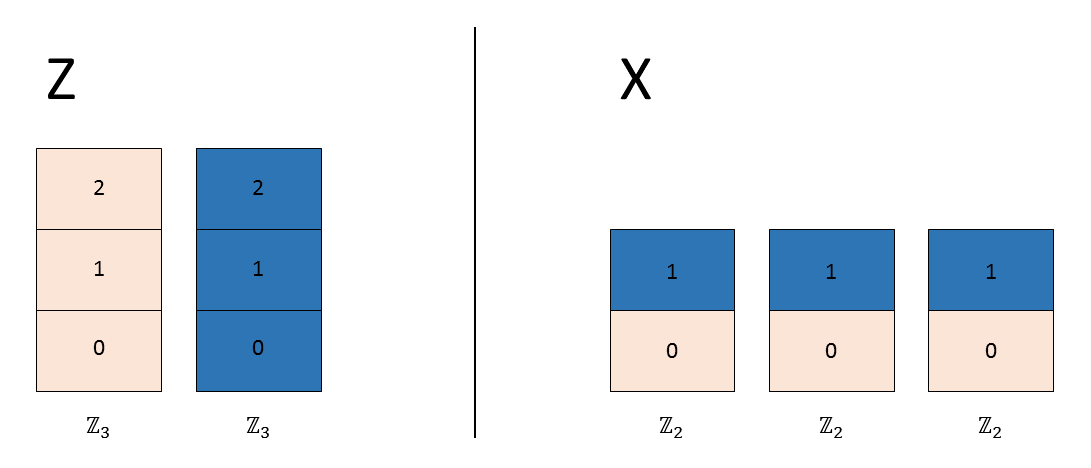
\includegraphics[height=10em,natwidth=1091,natheight=468,scale=1]{images/complexample.png}
\end{center}
\vspace{-14pt}
\caption[An example of two complementary bases on the system of six elements.]{An example of two complementary bases on the system of six elements. Here $Z=\mathbb{Z}_3\oplus\mathbb{Z}_3$ and $X = \mathbb{Z}_2\oplus\mathbb{Z}_2\oplus \mathbb{Z}_2$.  The two classical states of $Z$ are each three element subsets and are colored in pink and blue. The unbiased states of $X$ to which they correspond are colored to match.
}
\label{complEx}
\end{figure}

\begin{corollary}[\cite{evans2009classifying}]
The \textbf{classical states} of a basis $Z = \bigoplus^{N}G$ are the subsets corresponding to the groups $G_0, G_1,...$ where we forget the group structure. They will often be denoted $\ket{G_i}$.
\end{corollary}

\begin{corollary}[\cite{evans2009classifying}]
The \textbf{unbiased states} for a basis $Z = \bigoplus^{N}G$ are subsets $U$ such that for a fixed $g\in G$, $\ket{U} = \bigoplus^{N}\{g\}$.
Thus there is exactly one element in each unbiased $U$ from each component $G_i$ of $Z$.
\end{corollary}

\begin{example}
Take $Z = \mathbb{Z}_2\oplus\mathbb{Z}_2=\{0_a,1_a,0_b,1_b\}$. The classical states of $Z$ are $\ket{G_a}=\ket{0_a\vee1_a}$ and $\ket{G_b}=\ket{0_b\vee1_b}$.  The unbiased states of $Z$ are $\ket{U_0}=\ket{0_a\vee0_b}$ and $\ket{U_1}=\ket{1_a\vee1_b}$.
\end{example}

It is easy to check that bases as specified by Theorem \ref{thm:compl} have the property that each classical state $\ket{G_i}$ of the basis $Z$ corresponds to one unbiased state of $X$ and vice versa.
This allows us to call these bases mutually unbiased, i.e. complementary~\cite{evans2009classifying}.
\subsubsection*{Phases}

Phases are also defined in this relational setting.  In Hilbert space quantum mechanics a quantum phase for an n-dimensional system is given by the vector
\begin{align*}
\left(\begin{array}{c}
e^{i\phi_1} \\
\vdots \\
e^{i\phi_n}
\end{array}
\right).
\end{align*}
These quantum phases form an abelian group and can be applied as phase gates.
Their relational counterparts are described by the following lemma from \cite{cqm-notes}:
\begin{lemma}
For a basis $Z=\bigoplus_i^NG_i$, the \textbf{phase group} $B(Z)$ is given by $\prod_i^NG_i$.
\end{lemma}

\begin{example}
Consider the basis $\mathbb{Z}_2\oplus\mathbb{Z}_2$ for the four element system $\{00,01,10,11\}$.  Let $|\psi\rangle$ be the state $|00\vee10\rangle$. Application of the phase $11$ results in
\[ 11|00\vee10\rangle = |11\vee01\rangle . \]
\end{example}

We are also able to interpret GHZ states and density matrices in sets and relations.

\begin{defn}
For a basis $Z$, a \textbf{GHZ} state is given by
\[ GHZ_Z \; := \{\;(a,b,c)\;|\;\ \forall \;a,b,c \in Z,\;a\bullet_Zb\bullet_Zc = \mbox{id}_{G_i}\mbox{ for some } i\;\}.  \]
\end{defn}

\begin{defn}
For a state $|\psi\rangle$, the \textbf{density matrix} $|\psi\rangle\langle\psi|$ is given by the relation $xRy$ s.t. $x,y\in \psi$.
\end{defn}

\subsubsection*{The Model QCRel}

\begin{defn}
Axioms 1-4, and subsequent definitions, specify the operational generalized compositional theory for \textbf{quantum computation in relations: QCRel}.
\end{defn}

By the oGCT construction, this clearly makes QCRel a model of quantum computation in sets and unitary relations. It is worth noting that QCRel can be simply viewed as a local hidden variable theory. Consider the set $H$ to be the set of ontic states such that for $\phi\subseteq H$ the state $\ket{\phi}$ is non-deterministically in any of the ontic states in the subset $\phi$.  From this perspective, QCRel provides a non-deterministic local hidden variable model for computational aspects of quantum mechanics \cite{abramsky2012operational}. This means that protocols exist for entanglement, teleportation, and, as we show in this section, some familiar blackbox algorithms.

\subsection{Unitary Oracles}

In order to model blackbox quantum algorithms in this setting, we must define the oracles themselves.
We do this by building up from an abstract definition of the controlled-not gate in the literature. Let the gray classical structure on a system $A$ be given by a basis $Z=\bigoplus^{|H|}G$ and the white classical structure be a basis $X=\bigoplus^{|G|}H$. The comonoid for the gray dot is then the relation $\tinycomult[graydot]:A\to A\times A$ that for $x,a,b\in H$ is given by
\[ \{(x,(a,b))~|~a\bullet_Zb=x\}. \]

\begin{defn}[\cite{zeng2014abstract}]
\label{eq:generalizedcnotrel}
The abstract controlled-not is given by a composition of the comonoid for Z and the monoid for X:
\begin{equation}
\label{eq:cnot_rel}
\,\,
\begin{aligned}
\begin{tikzpicture}[yscale=0.6, xscale=0.6,string]
\node (b) [graydot] at (0,0) {};
\node (w) [whitedot] at (1,1) {};
\draw (-0.75,2) to [out=down, in=left] (b.center);
\draw (b.center) to [out=right, in=left] (w.center);
\draw (w.center) to (1,2);
\draw (b.center) to (0,-1);
\draw (w.center) to [out=right, in=up] (1.75,-1);
\end{tikzpicture}
\end{aligned}
\qquad \qquad\qquad
\begin{tabular}{l}
\mbox{CNOT:} $H\times H\to H\times H ::$ \\
$\{((x,y),(a,b\circ_Xy))~|~a\bullet_Zb=x\}.$ \\
\end{tabular} 
\end{equation}
\end{defn}
It can be shown that in the traditional quantum setting of Hilbert spaces and linear maps, this exactly corresponds to the usual controlled-not. This also leads to the following useful theorem, which can be abstractly proved.

\begin{theorem}[Complementarity via a unitary \cite{zeng2014abstract}]
\label{thm:complementarityunitary}
  Two symmetric dagger-Frobenius algebras are complementary if and only if the abstract controlled-not from Definition \ref{eq:generalizedcnotrel} is unitary.
\end{theorem}

\noindent This allows us to prove the following about  complementary bases in QCRel.
\begin{theorem}
Two bases (Z and X) in QCRel are complementary, in the sense of Theorem~\ref{thm:compl}, if and only if the relation in \eqref{eq:cnot_rel} is a bijection.
\end{theorem}
\begin{proof}
The relevant relation can clearly be seen to be the composite in Definition~\ref{eq:generalizedcnotrel} as:
\begin{align}
\{((a,b,y),(a,b\circ_Xy))\} \circ \{((x,y),(a,b,y))~|~a\bullet_Zb=x\}.
\end{align}
Thus the abstract proof of\ Theorem \ref{thm:complementarityunitary} from \cite{zeng2014abstract} goes through unchanged.
\end{proof}

An oracle is then introduced as a controlled-not where we have embedded a particular kind of relation that abstractly must be a self-conjugate comonoid homomorphism \cite{zeng2014abstract}. We construct such relations in the following lemmas.

\begin{defn}
Let $G$ and $H$ be groupoids with with groupoid multiplications $\bullet_G$ and $\bullet_H$ respectively. Let $\mbox{id}_{G}=\bigcup_{X\in\mbox{Ob}(G)}\mbox{id}_X$ and similarly define $\mbox{id}_{H}$. A \textbf{groupoid homomorphism relation} $R:G\to H$ obeys the following condition for $g_1,g_2\in G$:
%two conditions for $g_1,g_2\in G$ and $h_1,h_2\in H$:
\begin{align}
R(g_1\bullet_Gg_2) &= R(g_1)\bullet_HR(g_2) %\\
%R(\mbox{id}_G) &= \mbox{id}_H
\end{align}
\end{defn}
\noindent Note that while this in many ways resembles a groupoid homomorphism, it is actually a weakening of this notion, in that groupoid homomorphism relations are not required to be total functions and have no explicit requirement on their identity morphisms.

\begin{defn}
A \textbf{monoid homomorphism relation} is a monoid homomorphism in \cat{Rel}. Specifically, let $A$ and $B$ be sets equipped with monoids $(A,\tinymult[whitedot],\tinyunit[whitedot])$ and $(B,\tinymult[blackdot],\tinyunit[blackdot])$ respectively. A relation $r:A\to B$ is a monoid homomorphism when is obeys the following two conditions:
\begin{align}
\label{eq:monone}
r\circ\tinymult[whitedot] &= \tinymult[blackdot]\circ(r\times r) 
\end{align}
\begin{align}
\label{eq:monunit}
r\circ\tinyunit[whitedot] &= \tinyunit[blackdot]
\end{align}
A \textbf{comonoid homomorphism relation} is defined similarly, using duals of the above conditions.
\end{defn}

\begin{lemma}
\label{lem:mongrphom}
A groupoid homomorphism relation that is surjective on objects is a monoid homomorphism relation.
\end{lemma}
\begin{proof}
Throughout this proof we refer to a groupoid as a category where the elements of the groupoid are the morphisms.  From this perspective a group is a groupoid with a single object. Consider a groupoid homomorphism relation $R:G\to H$ on objects $X,A,B$ of $G$ and morphisms $f$ of $G$.
In order to show that $R$ is a monoid homomorphism relation we first show that it preserves the unit~\eqref{eq:monunit}. We have $R(\bigcup_{X\in\mbox{Ob}(G)} \mbox{id}_X) = \bigcup_{Y\in\mbox{Ob}(H)} \mbox{id}_Y$. Recall that for a set $A$,  $R(A)=\bigcup_{a\in A} R(a)$. It is that case that
\begin{align}
R(\bigcup\nolimits_{X\in\mbox{Ob}(G)} \mbox{id}_X) &= \bigcup\nolimits_{X\in\mbox{Ob}(G)}R(\mbox{id}_X) = \bigcup\nolimits_{X\in\mbox{Ob}(G)}\mbox{id}_{R(X)} \quad \mbox{def. of group hom. rel.} \\
&= \bigcup\nolimits_{R(X)\in\mbox{Ob}(G)}\mbox{id}_{R(X)} = \bigcup\nolimits_{{Y\in\mbox{Ob}(H)}}\mbox{id}_{Y} \qquad \mbox{surjective on objects}
\end{align}
where we have used the fact that $R$ is surjective on objects, which implies that every object of $H$ is in the image of $R$ and that $|\mbox{Ob}(G)|\ge|\mbox{Ob}(H)|$.

The second monoid homomorphism condition~\eqref{eq:monone} is to preserve multiplication, i.e. that for subsets $K$ and $J$ of $G$ we have
\begin{align}
R(K+_GJ)=R(K)+_HR(J).
\end{align}

\noindent Here we recall that for two sets $A$ and $B$, $A+B=\{a + b | a \in A\mbox{ and } b \in B\}$. Thus,
\begin{align}
R(K+_GJ) &= R(\bigcup\nolimits_{k\in K,j\in J}k+_Gj) = \bigcup\nolimits_{k\in K,j\in J}R(k+_Gj) \\
&= \bigcup\nolimits_{k\in K,j\in J}R(k)+_HR(j) \qquad \mbox{def. of group hom. rel.}\\
&= R(K)+_HR(J).
\end{align}
This completes the proof.
\end{proof}

We then dualize the proof of Lemma \ref{lem:mongrphom} to conclude that:
\begin{lemma}
\label{lem:classicalRelation}
Let $F:H\to G$ be a functor such that $F^{\mbox{\tiny op}}$ is a groupoid homomorphism relation that is surjective on objects. $F$ is a comonoid homomorphism relation.
\end{lemma}
\noindent We call these comonoid homomorphism relations \textbf{classical relations}. These are relations that properly preserve the structure of the bases where classical data is embedded.  In the quantum case they take basis elements to basis elements. Some examples in QCRel are listed in Appendix \ref{app:clRel}. In order to define unitary oracles, we also need these relations to be self-conjugate:

\begin{defn}[\cite{zeng2014abstract}]
In a monoidal dagger-category, a comonoid homomorphism \mbox{$f:\blackcomonoid{A} \to \graycomonoid{B}$} between dagger-Frobenius comonoids is \textbf{self-conjugate} when the following property holds:
\begin{equation}
\label{eq:comonoidhomomorphismselfconjugate}
\begin{aligned}
\begin{tikzpicture}[yscale=0.8, xscale=0.8, thick]
\node [morphism] (f) at (2,1) {$f$};
\draw (0,-1) to [out=up, in=left, in looseness=0.9] (1,2) node [graydot] {} to (1,2.5) node [graydot] {};
\draw (1,2) to [out=right, in=up] (f.north);
\draw (f.south) to [out=down, in=left] (3,0) node [blackdot] {} to [out=right, in=down, out looseness=0.9] (4,3);
\draw (3,0) to (3,-0.5) node [blackdot] {};
\node [graydot] at (1,2) {};
\end{tikzpicture}
\end{aligned}
\quad=\quad
\begin{aligned}
\begin{tikzpicture}[yscale=1.05, xscale=0.8, thick]
\node (f) at (0,0) [morphism] {$f^{\dagger}$};
\draw (0,-1.5) to (f.south);
\draw (f.north) to (0,1.5);
\end{tikzpicture}
\end{aligned}
\end{equation}
\end{defn}
The meaning of this equation in relations is explicated in the following lemma.

\begin{lemma}
All classical relations $f:Z^A\to Z^B$ between groupoids $Z^A=\bigoplus^NG$ and $Z^B=\bigoplus^{N'}H$ are self-conjugate.
\end{lemma}
\begin{proof}
In QCRel, our dagger-Frobenius structures are groupoids and, if they are complementary to some other groupoid, then they are of the form $Z^A=\bigoplus^NG$ and $Z^B=\bigoplus^{N'}H$. We annotate the definition of self-conjugacy for some arbitrary element $(g,n)$, the element $g$ from the $n$-th group. Recall that $f^{\dagger}=f^{-1}$ in QCRel.
\begin{equation}
\begin{aligned}
\begin{tikzpicture}[yscale=0.9, xscale=1.3, thick]
\node [morphism] (f) at (2,1) {$f$};
\draw (0,-1) to [out=up, in=left, in looseness=0.9] (1,2) node [graydot] {} to (1,3.3) node [graydot] {};
\draw (1,2) to [out=right, in=up] (f.north);
\draw (f.south) to [out=down, in=left] (3,-0.7) node [blackdot] {} to [out=right, in=down, out looseness=0.9] (4,3);
\draw (3,-0.7) to (3,-2) node [blackdot] {};
\node [graydot] at (1,2) {};
\node at (0,-1.25) {\small $(g,n)$};
\node at (-0.25,1.5) {\small $(g,n)$};
\node at (0.9,2.65) {\small $\{(id_G,j) | 1 \leq j \leq N\}$};
\node at (2.5,1.7) {\small $(g^{-1},n)$};
\node at (2.1,-0.15) {\small $f^{-1}(g^{-1},n)$};
\node at (4.3,0) {\small $\left[f^{-1}(g^{-1},n)\right]^{-1}$};
\node at (2.95,-1.4) {\small $\{(id_H,k) | 1 \leq k \leq N'\}$};
\end{tikzpicture}
\end{aligned}
\quad=\quad
\begin{aligned}
\begin{tikzpicture}[yscale=1.2, xscale=1.3, thick]
\node (f) at (0,0) [morphism] {$f^{-1}$};
\draw (0,-1.5) to (f.south);
\draw (f.north) to (0,1.5);
\node at (0,-2) {\small $(g,n)$};
\node at (0,2) {\small $f^{-1}(g,n)$};
\end{tikzpicture}
\end{aligned}
\end{equation}
Thus, a relation $f$ is self-conjugate if and only if for all elements $(g,n)$ it is the case that $[f^{-1}(g^{-1},n)]^{-1}=f^{-1}(g,n)$. From Lemma \ref{lem:classicalRelation} the converse of the classical relation $f$ is a monoid homomorphism relation whose multiplication is the groupoid operation, so this condition will hold.
\end{proof}

Classical relations, as self-conjugate comonoid homomorphisms, lead to unitary oracles.

\begin{defn}[Oracle \cite{zeng2014abstract}]
\label{oracle}
Given a groupoid $Z^A:\blackcomonoid{A}$, a pair of complementary groupoids $Z^B:\graycomonoid{B}$ and $X^B:\whitecomonoid{B}$, and a classical relation $R : \blackcomonoid{A} \to \graycomonoid{B}$, an \textbf{oracle} is defined to be the following endomorphism of~$A \times B$:
\begin{equation}
\label{eq:oraclerel}
\begin{aligned}
\begin{tikzpicture}[string,xscale=0.9, yscale=0.7]
    \node (dot) [blackdot] at (0,1) {};
    \node (f) [morphism] at (0.7,2) {$R$};
    \node (m) [whitedot] at (1.4,3) {};
\draw (0,0.25)
        node [below] {$A$}
    to (0,1)
    to [out=left, in=south] (-0.7,2)
    to (-0.7,3.75)
        node [above] {$A$};
\draw (0,1)
    to [out=right, in=south] (f.south);
\draw  (f.north)
    to [out=up, in=left] (1.4,3)
    to [out=right, in=up] +(0.7,-1)
    to (2.1,0.25)
        node [below] {$B$};;
\draw (m.center) to +(0,0.75) node [above] {$B$};
\end{tikzpicture}
\end{aligned}
\qquad \qquad
\begin{align*}
&\mbox{\emph{OracleRel(R)}}:A\times B\to A\times B  ::\\
&\{((x,y),(a,c\circ_Xy))~|~ \\ &\hspace{50pt}\exists b\in A, s.t.~a\bullet_{Z^A}b=x\mbox{\emph{ and }} bRc\}. \\
\end{align*}
\end{equation}
\end{defn}
\begin{theorem}
\label{thm:familyofunitaries}
Oracles are unitary.
\end{theorem}
\begin{proof}
Proved in the abstract setting for Definition \ref{oracle} in \cite{zeng2014abstract}, when $R$ is a self-conjugate comonoid homomorphism.  Though there are others, classical relations $R$ are necessary and sufficient in our cases as the algorithms that follow additionally require that the comonoids be part of classical structures.
\end{proof}

\begin{corollary}
OracleRel is a bijection.
\end{corollary}
\begin{proof}
This follows directly from Theorem \ref{thm:familyofunitaries} and Corollary \ref{cor:bijections}.
\end{proof}

\subsection{The Fourier Transform in Relations}
\label{sec:RelFT}

In Section~\ref{section_RelFT}, we saw that there are several perspectives on the Fourier Transform in \cat{FRel}, only some of which are nontrivial. In this section we take the operational perspective on the generalized quantum Fourier transform whose definition is motivated through the relationship between classical and unbiased states of two bases.  For abelian groups $G$ and $H$, consider two groupoids $Z=\bigoplus^{|H|}G$ and $X=\bigoplus^{|G|}H$ to be complementary bases of the same system.

\begin{defn}
\label{def:FTRel}
The \textbf{quantum Fourier transform in relations} corresponds to preparing classical states of $Z$ and measuring them against classical states of $X$.
%is an isomorphism from the classical states of $Z$ to the unbiased states %of $X$, i.e.
%\begin{align*}
%\{G_h\}\mapsto \{h_g|\forall g\in G\}
%\end{align*}
\end{defn}

\begin{example}
Take $G=\mathbb{Z}_2=\{0,1\}$, $H=\mathbb{Z}_1=\{\star\}$, $Z = G$ and $X=H\oplus H = \{ (\star,0),(\star,1) \}$. The computational basis is the family $\ket{H_g}_{g\in G}$ of classical states for $X$, i.e. $H_0 = \{(\star,0)\}$ and $H_1 = \{(\star,1)\}$. The quantum Fourier basis is a single classical state $G_\star = \{(\star,0), (\star,1)\}$ for $Z$. In this case all states can be prepared in the computational basis, but  measurement in the quantum Fourier basis is trivial.
\end{example}

\begin{example}
Take $G=\mathbb{Z}_2=\{0,1\}$, $H=\mathbb{Z}_2=\{a,b\}$, $Z = G \oplus G = \{ (0,0),(1,0),(0,1),(1,0)\}$ and $X= H \oplus H = \{ (a,a), (b,a), (a,b), (b,b) \}$. The computational basis is the family $\ket{H_g}_{g \in G}$ of classical states for $X$, i.e. $H_0 = \{(a,a),(b,a)\}$ and $H_1 = \{(a,b),(b,b)\}$. The quantum Fourier basis is the family $\ket{G_h}_{h\in H}$ of classical states for $Z$, i.e. $G_a = \{(0,0),(0,1)\}$ and $G_b = \{(1,0),(1,1)\}$.
\end{example}

See Section~\ref{sec:strcomplFT} and~\cite{gogioso2015fourier} to fully motivate this definition of the Fourier transform in QCRel and for its relationship to the usual Hadamard and Fourier transforms for Hilbert spaces and linear maps.

\subsection{The Deutsch-Jozsa Algorithm in QCRel}

The well known Deutsch-Jozsa algorithm is an early quantum algorithm that demonstrates a speedup over exact classical computation \cite{DJAlg1992}. It takes as input a function promised to be either constant or balanced and returns which, deterministically using only a single oracle query. In this section, we model the algorithm's steps in QCRel just as it is implemented with Hilbert spaces and linear maps. This approach is somewhat dual to the usual one where different algorithms are compared on the same problem. Here we run the same abstract protocol (implemented in a different model) with the same query complexity and compare the different problems that it solves.

To run this algorithm in QCRel we use two systems.  System $A$ has cardinality $n$ and system $B$ has cardinality $\ge 2$. Take $Z^A=\bigoplus^{|H^{A}|}G^A$ and $X^A=\bigoplus^{|G^{A}|}H^A$ to be complementary bases of $A$. Take $Z^B=\bigoplus^{|H^{B}|}G^B$ and $X^B=\bigoplus^{|G^{B}|}H^B$ to be complementary bases of $B$, such that $X^B$ has at least two classical states. In analogy with the usual specification, the algorithm proceeds with the following steps.
\begin{enumerate}
\item Prepare $A$ in the zero state $|G^{A}_0\rangle$. Prepare $B$ in the state given by the second classical state of $Z^B$, i.e. $|G^B_1\rangle$.

\item Apply the Fourier transform, as given by Definition \ref{def:FTRel}, to each system, resulting in states $\ket{H_0^A}$ and $\ket{H_1^B}$ respectively.

\item Apply an oracle \eqref{eq:oraclerel}, built from a classical relation $f:Z^A\to Z^B$.

\item Again apply the Fourier transform to system $A$ and then measure it in the $Z$ basis.
\end{enumerate}

\noindent This sequence of steps is an instance in sets and relations of the abstract Deutsch-Jozsa algorithm from \cite{vicary-tqa}, which translates to the following relation, where we have already applied the Hadamard map  to the input and output. See~\eqref{eq:postFT}.

\begin{equation}
\label{eq:reldj}
\begin{aligned}
\begin{tikzpicture}[string, yscale=1, xscale=1]
    \node (dot) [blackdot] at (0,1) {};
    \node (f) [morphism] at (0.7,2) {$f$};
    \node (m) [whitedot] at (1.4,3) {};
\draw (0,0.25)
        node [blackdot] {}
    to (0,1)
    to [out=left, in=south] (-0.7,2)
    to (-0.7,3.75)
        node [blackdot] {};
\draw (0,1)
    to [out=right, in=south] (f.south);
\draw  (f.north)
    to [out=up, in=left] (1.4,3)
    to [out=right, in=up] +(0.7,-1)
    to (2.1,0.25)
        node [graydot] {};
\node at (2.15,0.25) [anchor=west] {$|H^B_1\rangle$};
\node at (0.05,0.25) [anchor=west] {$|H^A_0\rangle$};
\node at (-0.65,3.75) [anchor=west] {$\langle H^A_0|$};
\draw (m.center) to +(0,0.75)
        node [above] {};
\draw [thin, dashed] (-1.25,0.7) to (7.5,0.7);
\draw [thin, dashed] (-1.25,3.3) to (7.5,3.3);
\node at (3.5,0) [anchor=west] {\small Prepare initial states and apply Hadamard};
\node at (3.5,2) [anchor=west] {\small Apply a unitary map};
\node at (3.5,4) [anchor=west] {\small Apply Hadamard and measure the first system};
\end{tikzpicture}
\end{aligned}
\end{equation}
that is explicitly written as:
\begin{align*}
\mbox{DJAlg}(f)&::\{\star\}\times \{\star\} \to \{\star\}\times B \\
&=
\bra{H_0^A}\times{\mbox{id}_B}\circ\mbox{OracleRel}(f)\circ\ket{H^A_0}\times\ket{H^B_1}
\\ &=
\{((\star,\star),(\star,z))\;|\; 
  z\in H_1^B \mbox{ and } \exists y\in H_0^A, \mbox{ s.t. }yfz\},
\end{align*}
where we have made the simplification of \eqref{eq:reldj} following \cite{vicary-tqa}.

\begin{theorem}[\cite{vicary-tqa}]
\label{def:bc}
In any dagger compact category with complementary bases, the algorithm in Equation \ref{eq:reldj} will, with a single oracle query, distinguish \textbf{constant} and \textbf{balanced} classical relations $f:Z^A\to Z^B$ according to the following abstract definitions. Here $\ket{x}$ is a classical point of $Z^A$ and the zero scalar $0$ is, in \cat{Rel}, the empty relation:
\begin{equation}
\label{eq:bc}
\mbox{\\ constant}:\quad
\begin{aligned}
\begin{tikzpicture}[scale=1]
\node (f) [morphism] at (0,0) {$f$};
\draw (0,-1) to (f.south);
\draw (f.north) to (0,1);
\end{tikzpicture}
\end{aligned}
\;=\;
\begin{aligned}
\begin{tikzpicture}[scale=1]
\draw (0,-1) to (0,-.4)
    node [blackdot] {};
\draw (0,0.5) node [state] {$x$} to (0,1);
\end{tikzpicture}
\end{aligned}
=\ket{x}\circ\tinycounit[blackdot]
\qquad\qquad \mbox{balanced:\quad}
\begin{aligned}
\begin{tikzpicture}[string, scale=1]
\node [morphism] (f) at (0,0) {$f$};
\draw (0,-0.85) node [blackdot] {} to (f.south);
\draw (f.north) to (0,0.75) node [graydot, hflip] {};
\node at (0.05,0.75) [anchor=west] {$2$};
\end{tikzpicture}
\end{aligned}
\quad=\quad
0, \vspace{-5pt}
\end{equation}
where 
\begin{tikzpicture}[string, yscale=1]
\draw (f.north) to (0,0.75) node [graydot, hflip] {};
\node at (0.05,0.75) [anchor=west] {$2$};
\end{tikzpicture} is the dagger adjoint of the second classical state of $X^B$.
\end{theorem}
That these definitions coincide with the usual ones for constant and balanced functions is shown in \cite{vicary-tqa}. In QCRel, the effect 
\begin{tikzpicture}[string,scale=0.75]
\draw (f.north) to (0,0.75) node [blackdot, hflip] {};
%\node at (0.05,0.75) [anchor=west] {$2$};
\end{tikzpicture} is $\langle H^A_1|$, which acts as a measurement of system $A$ after applying the oracle.
We illustrate the details of the QCRel model of this algorithm by example and then with general definitions.

\begin{example}
Take $A=\{0,1,2,3\}$ and $B=\{a,b,c,d\}$ to be four element systems. We define complementary bases on these systems as the following:
\begin{align*}
\begin{tabular}{|c|c|}\hline
System $A$ & System $B$ \\\hline
$Z^A = \mathbb{Z}_2\oplus\mathbb{Z}_2 \mbox{~~s.t.}$ & $Z^B = \mathbb{Z}_2\oplus\mathbb{Z}_2\mbox{~~s.t.}$ \\
$G_0^A=\{0,1\},G_1^A=\{2,3\}$ & $G_0^B=\{a,b\},G_1^B=\{c,d\}$ \\ \hline
$X^A = \mathbb{Z}_2\oplus\mathbb{Z}_2 \mbox{~~s.t.}$ & $X^B = \mathbb{Z}_2\oplus\mathbb{Z}_2\mbox{~~s.t.}$ \\
$H_0^A=\{0,2\},H_1^A=\{1,3\}$ & $H_0^B=\{a,c\},H_1^B=\{b,d\}$ \\ \hline
\end{tabular}
\end{align*}


From Equation \ref{eq:bc}, we then define constant and balanced classical relations using the following dictionary:
\begin{align}
\begin{aligned}
\begin{tikzpicture}[string]
\draw (0,0.2) to (0,0.75) node [blackdot, hflip] {};
\node at (0.05,0.75) [anchor=west] {};
\end{tikzpicture}
\end{aligned}
&\quad= \{(0,\star),(2, \star)\},  \quad \mbox{the adjoint of the first classical state of } X^A \\
\begin{aligned}
\begin{tikzpicture}[string]
\node (x) [state, xscale=0.75] at (0,0) {$x$};
\draw (0,0) to (0,0.5) {};
\end{tikzpicture}
\end{aligned}
&\quad= \{(\star,a),(\star,b)\}\mbox{ OR }\{(\star,c),(\star,d)\},  \quad \mbox{a classical state of }Z^B \\
\begin{aligned}
\begin{tikzpicture}[string]
\draw (0,0.2) to (0,0.75) node [graydot, hflip] {};
\node at (0.05,0.75) [anchor=west] {$2$};
\end{tikzpicture}
\end{aligned}
&\quad=\{(b,\star),(d, \star)\},  \quad \mbox{ adjoint of the second classical state of } X^B \\
\begin{aligned}
\begin{tikzpicture}[string]
\node (x) [blackdot] at (0,0) {};
\draw (0,0) to (0,0.5) {};
\end{tikzpicture}
\end{aligned}
&\quad= \{(\star,0),(\star,2)\},  \quad \mbox{the first classical state of } X^A
\end{align}

Thus there are two constant classical relations\footnote{A list of more example classical relations is given in Appendix \ref{app:clRel}.} $f:Z^A\to Z^B$, one for each classical state of $Z^B$. They are:
\begin{align*}
\{ (0,a),(0,b) ,(2,a),(2,b) \} \quad \mbox{and} \quad
\{ (0,c),(0,d), (2,c),(2,d) \}.
\end{align*}
By Definition \ref{def:bc}, balanced classical relations are those which do not relate $0$ or $2$ to either $b$ or $d$. There are four balanced classical relations for this example:
\begin{align*}
\{(0,c),(2,c),(1,d),(3,d)\} &\qquad \{(0,a),(1,b),(2,c),(3,d)\} \\
\{(2,a),(3,b),(0,c),(1,d)\} &\qquad \{(0,a),(2,a),(1,b),(3,b)\} \\
\end{align*}
For a classical relation promised to be in one of these two classes, we can distinguish which with a single oracle query.
\end{example}

We generalize these definitions of constant and balanced classical relations to the following:
\begin{defn}
\label{def:const}
Let $Z^A=\oplus^NG_i$. A \textbf{constant relation} $f:Z^{A}\to Z^{B}$ relates all id$_{G_i}$ to a single classical state of $Z^B$.
\end{defn}

\begin{defn}
\label{def:balanced}
A relation $f:Z^{A}\to Z^{B}$ is \textbf{balanced} when no element in the first classical state of $X^{A}$ is related to an element in the second classical state of $X^{B}$.
\end{defn}

\begin{theorem}
\label{thm:dj_speedup}
The Deutsch-Jozsa algorithm defined above distinguishes constant relations from balanced relations in a single oracle query.
\end{theorem}
\begin{proof}
This follows immediately from the abstract proof of the Deutsch-Jozsa algorithm in \cite{vicary-tqa}.
\end{proof}

This result shows that we are able to model the Deutsch-Jozsa algorithm in the nondeterministic classical setting of QCRel.

\subsection{Single-shot Grover's Algorithm}

The usual Grover's algorithm~\cite{grover1996fast} takes as input a set $S$ and an indicator function $f:S\to\{0,1\}$ and outputs an element $s\in S$ such that $f(s)=1$. Though the algorithm is usually probabilistic and runs a repeated series of ``Grover steps", here we consider the deterministic version that runs with a single step. In this section we will consider the generalization of the single-shot Grover algorithm where the codomain of the indicator function is allowed to be an arbitrary group~\cite{vicary-tqa}. Our setup requires the set $S$, as one system, as well as another system $B$. We define the basis $Z^{S}=\bigoplus^{|H^S|}G^S$ and $X^S=\bigoplus^{|G^S|}H^S$ on the $S$ system.  System $B$ has complementary bases $Z^B=\bigoplus^{|H^B|}G^B$ and $X^B=\bigoplus^{|G^B|}H^B$. Let $\ket{\sigma}$ be the first classical state of $X^B$, e.g. is $X^B=\mathbb{Z}_2\oplus\mathbb{Z}_2$ then $\ket{\sigma}=\{(\star,1),(\star,3)\}$, where $1$ and $3$ are the non-identity elements of that factors of $X^B$. Let $\bra{\rho}$ be the converse of a classical state of $X^S$. Recall that $\ket{G^S_0}=\{(\star,g)\,|\,g\in G^S\mbox{ is the first factor group of } Z^S\}$ is a classical point of $Z^S$, and that, by the complementary relationship of classical and unbiased points (Section~\ref{sec:RelFT}), $\ket{H^S_0}\isom\{(\star,\idm{G^S_i})\,|\,G^S_i\mbox{ is a factor group of } Z^S\}$.

In QCRel, the algorithm proceeds by the following steps:
\begin{enumerate}
\item Prepare system $S$ in the state $\ket{G_0}$ and system $B$ in the state $\ket{\sigma}$.

\item Apply the Fourier transform to system $S$, resulting in state $\ket{H^{S}_0}$.

\item Apply the oracle for a classical indicator relation $f:Z^S\to Z^B$.

\item Apply a diffusion relation $D:S\to S$ (defined below) to system $S$.

\item Measure system $S$ in the $X^S$ basis.

\end{enumerate}

The diagrammatic presentation for this procedure from \cite{vicary-tqa} is:
\begin{equation}
\label{eq:grovertopological}
\begin{aligned}
\begin{tikzpicture}[thick, xscale=1, yscale=0.5]
\begin{pgfonlayer}{foreground}
    \node (f) [smallbox, anchor=south, thick] at (0.7,2) {$f$};
\end{pgfonlayer}
    \node (dot) [blackdot] at (0,1) {};
    \node (m) [whitedot] at ([xshift=0.7cm, yshift=1cm] f.north) {};
\draw (0,-0.25)
        node [blackdot] (bdot) {}
    to (0,1)
    to [out=\nwangle, in=south] (-0.7,2)
    to ([yshift=1.4cm] m.center -| -0.7,1)
        node (rho) [state,hflip,yscale=1.5, xscale=1.1] {};
\node at (-0.7,5.9) {$\bra{\rho}$};
\draw (0,1)
    to [out=\neangle, in=south] (f.south)
    to (f.north)
    to [out=up, in=\swangle] +(0.7,1)
    to [out=\seangle, in=up] +(0.7,-1)
    to (2.1,-0.25)
        node [state,yscale=1.5, xscale=1.1] (sigmadag) {};
\node at (2.1,-1) {$\ket{\sigma}$};        
\draw (m.center) to (1.4,5.75)
        node [above] {};
\node [smallbox] at (-0.7,3.5) {$D$};
\node at (3.5,-0.25) [anchor=west] {Preparation};
\draw [thin, dashed] (-2,0.6) to (7,0.6);
\node at (3.5,2.25) [anchor=west] {Dynamics};
\draw [thin, dashed] (-2,4.5) to (7,4.5);
\node at (3.5,5) [anchor=west] {Measurement};
\end{tikzpicture}
\end{aligned}
\end{equation}

\noindent where numerical scalars have been dropped relative to that reference as there is only one non-zero scalar in QCRel.\footnote{Recall that scalars in a monoidal category with identity object $I$ are maps $s:I\to I$. Thus in \cat{Rel} $I=\{\star\}$, so the only scalars are the empty relation and the identity relation on the singleton set.} Recall that $\tinyunit[blackdot]:\{\star\}\to S$ relates the singleton to the elements of $H_0$ and that $\tinycounit[blackdot]$ is its relational converse. We will use the map $\tinyunit[blackdot]\circ\tinycounit[blackdot]:S\to S$ in the following definition. Here there is a special relation $D:S\to S$ called the diffusion operator and defined abstractly in \cite{vicary-tqa}:
\begin{equation}
\label{eq:difftopological}
\begin{aligned}
\begin{tikzpicture}[thick, scale=1]
\draw (0,0) node [below] {$S$} to node [smallbox] {$D$} (0,2) node [above] {$S$};
\end{tikzpicture}
\end{aligned}
\hspace{5pt}\;=\;\hspace{5pt}
\hspace{-5pt}
\begin{aligned}
\begin{tikzpicture}[thick, scale=1]
\draw (0,0) node [below] {$S$} to (0,2) node [above] {$S$};
\end{tikzpicture}
\end{aligned}
\;-\;
\begin{aligned}
\begin{tikzpicture}[thick, scale=1]
\draw (0,0) node [below] {$S$} to (0,0.7) node [blackdot] {};
\draw (0,2) node [above] {$S$} to (0,1.3) node [blackdot] {};
\end{tikzpicture}
\end{aligned}
\qquad\qquad \qquad D := \{(x,x)\,|\,x\in S\}\bigtriangleup (H_0\times H_0)
\end{equation}
where the subtraction of two relations is given by the symmetric difference of their images. Explicitly then, the relational model for Grover's algorithm is:
\begin{align*}
\mbox{Grover}(f)&:\{\bullet\}\times \{\bullet\} \to \{\bullet\}\times B \\
&=
\bra{\rho}\times{\mbox{id}_B}\circ D\times{\mbox{id}_B}\circ\mbox{OracleRel}(f)\circ\ket{H^S_0}\times\ket{\sigma}
\\ &= \{((\bullet,\bullet),(\bullet,c\circ_{X}x))\;|\; \\
&\hspace{40pt}
 x\in\sigma,y\in\rho, \mbox{id}_{G_n},b,z\in S \mbox{ s.t. } z\bullet_{Z^S} b=\mbox{id}_{G_{n}} \mbox{ and } bfc,zDy\}
\end{align*}

\begin{theorem}
\label{thm:topgrovers}
Equation \ref{eq:grovertopological} is zero only for classical states of $X^S$ denoted $\ket{\rho}$ that satisfy the following equation:
\begin{equation}
\label{eq:zerocondition}
\sigma \circ f \circ \rho = \sigma \circ f \circ \ket{G_0}
\end{equation}
%\begin{equation}
%\label{eq:zerocondition}
%\begin{aligned}
%\begin{tikzpicture}[thick, scale=0.5]
%\draw (0,0) node [smallbox] {$\rho$} to (0,1.25) node [smallbox] {$R$} to %(0,2.5) node [smallbox] {$\sigma$};
%\end{tikzpicture}
%\end{aligned}
%\quad=\quad
%\begin{aligned}
%\begin{tikzpicture}[thick, scale=0.5]
%\draw (0,0) node [blackdot] {} to (0,1.25) node [smallbox] {$R$} to (0,2.5) %node [smallbox] {$\sigma$};
%\node [smallbox, draw=white, fill=none] at (0,0) {};
%\draw (0,0) to (0,0.5);
%\end{tikzpicture}
%\end{aligned}
%\end{equation}
\end{theorem}
\begin{proof}
Proven in \cite{vicary-tqa}. See Section 3.2 equation (34).
\end{proof}

Here $\ket{\sigma}$ is, in general, any fixed classical state of $X^B$. This allows a generalization of the single-shot Grover's algorithm where the cardinality of system $B$ is increased as investigated in \cite{vicary-tqa}.
Consequently, the LHS of Equation \ref{eq:zerocondition} tests if any element in the classical state $\ket{\rho}$ is related to any of the elements in $\ket{\sigma}$. The RHS tests if any of the elements of $G_0$ are related to $\ket{\sigma}$.

\begin{proposition}
The QCRel single-shot Grover algorithm only returns states $\ket{\rho}$ such that for all $h \in H^S_0$, $s\in\rho$ and $x\in \sigma$
\begin{align*}
h f x \quad = \quad \neg(s f x) .
\end{align*}
In other words, the only elements that can be possibilistically measured under the QCRel Born rule (Axiom~\ref{ax:relborn}) are elements of $S$ that have the opposite mapping to $\sigma$, under the relation $f$, than elements of $H^{S}_0$.
\end{proposition}
\begin{proof}
By Theorem \ref{thm:topgrovers} and definitions.
\end{proof}

\begin{example}
Let $S=\{0,1,2,3\}$ and choose $Z^S=\mathbb{Z}_2\oplus\mathbb{Z}_2$ and $X^S=\mathbb{Z}_2\oplus\mathbb{Z}_2$ as $G$ (black) and $H$ (white) bases respectively, so that $G^{S}_0=\ket{0\vee 1}$ and $H^S_0 = \ket{0\vee 2}$. Let $B$ be the same four element system with the bases $Z^B=\mathbb{Z}_2\oplus\mathbb{Z}_2$ and $X^B=\mathbb{Z}_2\oplus\mathbb{Z}_2$ and choose $\ket{\sigma}=\ket{1\vee 3}$. The diffusion operator is then given by
\begin{align*}
D &:= \{(0,0),(1,1),(2,2),(3,3)\}-\{(0,0),(0,2),(2,0),(2,2)\}
\\&=\{(1,1),(3,3),(0,2),(2,0)\}.
\end{align*}

In this case, $D$ happens to be a bijection, it is a unitary relation and thus a possible evolution in QCRel.\footnote{This will not be the case whenever $S$ has more than two factor groups. Unitarity is a stringent condition on processes in QCRel.} Let $f$ be the classical relation\footnote{See Appendix \ref{app:clRel} for a list of classical relations $\mathbb{Z}_2\oplus\mathbb{Z}_2\to\mathbb{Z}_2\oplus\mathbb{Z}_2$.} $\{(0,2),(2,2),(1,3),(3,3)\}$, where elements of $H^S_0$ are not related to elements of $\ket{\sigma}$. Thus the above algorithm will only return classical states of $X^{S}$ that \textit{are} related, under $f$,\ to $\ket{\sigma}$.  The only possible outcome state is $\ket{1\vee 3}$.
\end{example}

\begin{example}
This is the same as the above example, but take $f$ to be the classical relation $\{(0,0),(2,0),(0,1),(2,1)\}$. As an element of $H^S_0$ is related to $\ket{\sigma}$, the algorithm will return classical states of $X^S$ which are \emph{not} mapped to $\ket{\sigma}$, i.e. the state $\ket{1\vee3}$.
\end{example}

\subsection{The Groupoid Homomorphism Promise Algorithm}

This section models the group homomorphism algorithm from \cite{zeng2014abstract} in QCRel.  The quantum version of the algorithm takes as input a blackbox function $f:G\to A$ promised to be one of the homomorphisms between group $G$ and abelian group $A$.  It then outputs the identity of the homomorphism. In that paper the full identification algorithm is built up by multiple calls to an instance of the problem for cyclic groups.\footnote{Making use of the structure theorem for abelian groups to complete the general case.} It is this cyclic group subroutine that we consider here. In the relational setting we will move from groups to groupoids. Let groupoid $H$ be complementary to groupoid $G$ and groupoid $B$ be complementary to groupoid $A$. The QCRel GroupHomID algorithm then takes as input a groupoid isomorphism $f:G\to A$.   Let $\ket{\rho}$ be a classical states of $H$, and $\ket{\sigma}$ be a classical state of $B$. 

The algorithm has the following abstract specification~\cite{zeng2014abstract}:
\begin{align}
\label{eq:groupdIDAlg}
\begin{aligned}
\begin{tikzpicture}[string, scale=1]
    \node (dot) [blackdot] at (0,1) {};
    \node (f) [morphism] at (0.7,2) {$f$};
    \node (m) [whitedot] at (1.4,3) {};
    \node (topsig) [copoint, scale=1.3,anchor=south] at (-0.7,3.6) {$\ket{\rho}$};
\draw (0,0)
        node [blackdot] {}
    to (0,1)
    to [out=left, in=south] (-0.7,2)
    to (topsig.south);
\draw (0,1)
    to [out=right, in=south] (f.south);
\draw  (f.north)
    to [out=up, in=left] (1.4,3)
    to [out=right, in=up] +(0.7,-1)
    to (2.1,0.4)
        node [point, scale=1.3, anchor=north] {$\ket{\sigma}$};
\draw (m.center) to (1.4,4.4)
        node [above] {};
\draw [thin, dashed] (-1.25,0.7) to (7.5,0.7);
\draw [thin, dashed] (-1.25,3.3) to (7.5,3.3);
\node at (3,0) [anchor=west] {Prepare initial states};
\node at (3,2) [anchor=west] {Apply a unitary map};
\node at (3,4) [anchor=west] {Measure the left system};
\end{tikzpicture}
\end{aligned}
\end{align}
Let the factor groups of a groupoid $G$ be denoted $G_n$. This gives the following relational model for the algorithm:
\begin{align*}
\mbox{GroupHomID}(f)&:\{\bullet\}\times \{\bullet\} \to \{\bullet\}\times B \\
&=
\bra{\rho}\times{\mbox{id}_B}\circ \mbox{OracleRel}(f)\circ\ket{H_0}\times\ket{\sigma}
\\ &= \{((\bullet,\bullet),(\bullet,c\circ_{X}x))\;|\; \\
&\hspace{40pt}
x\in\sigma,y\in\rho, \mbox{id}_{G_n},b\in A \mbox{ s.t. } y\bullet_G b=\mbox{id}_{G_{n}} \mbox{ and } bfc\}
\end{align*}

\begin{theorem}
The algorithm defined by~\eqref{eq:groupdIDAlg} has output state $\ket{\rho}$ only when for some $x\in \rho$ and some $y\in \sigma$ we have $(y,x)\in f$.
\end{theorem}
\begin{proof}
The verification in \cite{zeng2014abstract} simplifies the algorithm in Equation \ref{eq:groupdIDAlg} to:
\begin{equation}
\begin{aligned}
\begin{tikzpicture}[string, scale=0.9]
\node (r) [state] at (0,2) {$\sigma$};
\node (s) [state, hflip] at (0,3.5) {$\rho$};
\node (f) [morphism] at (0,2.75) {$f^{-1}$};
\node (r2) at (1.5,3) [state] {$\sigma$};
\draw (s.south) to (f.north);
\draw (f.south) to (r.north);
\draw (r2.north) to +(0,0.5);
\end{tikzpicture}
\end{aligned}
\qquad= \quad \{(\bullet,(\bullet,x))\;|\;x f^{-1} y\;\mbox{for some } y\in\rho\},
\end{equation}
where we see that post-selection on the left hand system implies the theorem's condition via the QCRel Born rule (Axiom~\ref{ax:relborn}).
\end{proof}

\begin{theorem}
If $f$ is a groupoid isomorphism then the algorithm in Equation \ref{eq:groupdIDAlg} returns all states.
\end{theorem}
\begin{proof}
Groupoid isomorphisms relate every element of the domain to some element in the codomain and relate every element of the codomain to some element of the domain.
\end{proof}

\noindent Still, we can imagine running the algorithm from \eqref{eq:groupdIDAlg} where any classical relation $f$ is allowed as input to obtain non-trivial outcomes.

\section{Conclusion}
In this chapter we have investigated the structure of quantum algorithms using the oGCT perspective. We have contributed the following new results:
\begin{enumerate}
\item A definition of the Fourier Transform in general oGCTs along with abstract proofs of the Fourier Inversion Theorem, Pontryagin Duality, and the Convolution Theorem.
\item A definition of the Hadamard Transforms and an operational Quantum Fourier Transform in general oGCTs.
\item We use complementary observables to construct a unitary oracle in a general oGCT and provide an abstract proof of its unitarity.  We show an equivalence between the complementarity of those observables and the unitarity of this oracle.
\item We pose a new problem, the GROUPHOMID problem, and give a quantum algorithm for its solution with favorable query complexity over classical algorithms.
\item We provide models for the operation of quantum algorithms in non-deterministic classical computation by explicitly constructing the Deutsch-Jozsa algorithm, the single-shot Grover's algorithm, and the GROUPHOMID algorithm in the oGCT QCRel. Along the way we introduce an operational notion of a oGCT Fourier Transform in \cat{FRel} and characterize some self-conjugate comonoid homomorphisms in this category.
\end{enumerate}

The successes of this approach opens up new work to study more blackbox quantum algorithms at this level of abstraction. We discuss more details of the outlook for future work in Chapter~\ref{chap:outlook}. 


%\chapter{Sample Title}

Lorem ipsum dolor sit amet, consectetur adipiscing elit, sed do eiusmod tempor incididunt ut labore et dolore magna aliqua. Ut enim ad minim veniam, quis nostrud exercitation ullamco laboris nisi ut aliquip ex ea commodo consequat. Duis aute irure dolor in reprehenderit in voluptate velit esse cillum dolore eu fugiat nulla pariatur. Excepteur sint occaecat cupidatat non proident, sunt in culpa qui officia deserunt mollit anim id est laborum.

%now enable appendix numbering format and include any appendices
%\appendix
%\chapter{Classical Relations}
\label{app:clRel}

In this appendix we list examples of classical relations as calculated by a Mathematica package available at: 
{\small https://github.com/willzeng/GroupoidHomRelations}
\begin{align*}
\begin{tabular}{lcl}
Classical relations $\mathbb{Z}_3\to\mathbb{Z}_3$:  & \hspace{60pt} & Classical relations $\mathbb{Z}_4\to\mathbb{Z}_4$:  \\[-10pt]
\begin{tabular}{l}
\{(0,0),(0,1),(0,2)\} \\
\{(0,0),(1,1),(2,2)\} \\
\{(0,0),(1,2),(2,1)\} 
\end{tabular} & &
\begin{tabular}{l}
\\
\{(0,0),(0,1),(0,2),(0,3)\} \\
\{(0,0),(1,1),(2,2),(3,3)\} \\
\{(0,0),(2,1),(0,2),(2,3)\} \\
\{(0,0),(3,1),(2,2),(1,3)\} 
\end{tabular}
\end{tabular}
\end{align*}
\\
\noindent The classical relations from  $\mathbb{Z}_2\oplus\mathbb{Z}_2\to\mathbb{Z}_2\oplus\mathbb{Z}_2$ are:
\begin{align*}
\begin{tabular}{cc}
\{(0,2),(2,2),(1,3),(3,3)\} &\qquad \{(0,0),(1,1),(2,2),(3,3)\} \\
\{(0,2),(2,2),(1,3),(2,3)\} &\qquad \{(0,0),(1,1),(2,2),(2,3)\} \\
\{(0,2),(2,2),(0,3),(3,3)\} &\qquad \{(0,0),(0,1),(2,2),(3,3)\} \\
\{(0,2),(2,2),(0,3),(2,3)\} &\qquad \{(0,0),(0,1),(2,2),(2,3)\} \\
\{(2,0),(3,1),(0,2),(1,3)\} &\qquad \{(0,0),(2,0),(1,1),(3,1)\} \\
\{(2,0),(3,1),(0,2),(0,3)\} &\qquad \{(0,0),(2,0),(1,1),(2,1)\} \\
\{(2,0),(2,1),(0,2),(1,3)\} &\qquad \{(0,0),(2,0),(0,1),(3,1)\} \\
\{(2,0),(2,1),(0,2),(0,3)\} &\qquad \{(0,0),(2,0),(0,1),(2,1)\} \\
\end{tabular}
\end{align*}
\newpage
\section{Mathematica Code}
\begin{lstlisting}[language=Mathematica]
(* This code generates groupoid homomorphisms in the category
 of relations *)
(* by William Zeng 2015 *)
(* william.zeng@cs.ox.ac.uk *)
(* Available at https://github.com/willzeng/GroupoidHomRelations *)

Groupoid Definitions

These multiplication tables define whatever groupoid 
homomorphisms you are considering. It is prepopulated
with some usual small ones

(* Define the cyclic group multiplication *)
(* INPUT: Integers 1,1 *)
(* OUTPUT: Integer 2*)
z3[x_, y_] := ({
      {0, 1, 2},
      {1, 2, 0},
      {2, 0, 1}
     })[[x + 1]][[y + 1]];
(* This defines multiplication on a set of inputs *)
(* INPUT: Integer sets {1,2},{2}*)
(* OUTPUT: Integer set {0,2}*)
z3Set[X_, Y_] := Union[Flatten[
    Table[
     Table[
      z3[X[[x]], Y[[y]]]
      , {x, 1, Length[X]}]
     , {y, 1, Length[Y]}]
    ]];
z4[x_, y_] := ({
      {0, 1, 2, 3},
      {1, 2, 3, 0},
      {2, 3, 0, 1},
      {3, 0, 1, 2}
     })[[x + 1]][[y + 1]];
z4Set[X_, Y_] := Union[Flatten[
    Table[
     Table[
      z4[X[[x]], Y[[y]]]
      , {x, 1, Length[X]}]
     , {y, 1, Length[Y]}]
    ]];

(* a is undefined *)
z2z2[x_, y_] := ({
      {0, 1, {}, {}},
      {1, 0, {}, {}},
      {{}, {}, 2, 3},
      {{}, {}, 3, 2}
     })[[x + 1]][[y + 1]];
z2z2Set[X_, Y_] := Union[Flatten[
    Table[
     Table[
      z2z2[X[[x]], Y[[y]]]
      , {x, 1, Length[X]}]
     , {y, 1, Length[Y]}]
    ]];

z2z2z2[x_, y_] := ({
      {0, 1, {}, {}, {}, {}},
      {1, 0, {}, {}, {}, {}},
      {{}, {}, 2, 3, {}, {}},
      {{}, {}, 3, 2, {}, {}},
      {{}, {}, {}, {}, 4, 5},
      {{}, {}, {}, {}, 5, 4}
     })[[x + 1]][[y + 1]];
z2z2z2Set[X_, Y_] := Union[Flatten[
    Table[
     Table[
      z2z2z2[X[[x]], Y[[y]]]
      , {x, 1, Length[X]}]
     , {y, 1, Length[Y]}]
    ]];

(* Relational evaluation method *)
(* INPUT: Relation R = {{0,0},{1,1},{2,2},{2,3}}; 
and argument x=2*)
(* OUTPUT: List of Integers {2,3}*)
eval[R_, x_] := Map[#[[2]] &, Select[R, #[[1]] == x &]];
(* All possible relations *)
(*allRelations = Subsets[Tuples[{0,1,2,3},2]];*)

Choose Groupoids

(*Set the size of the domain and coDomain*)
nD = 4; (*Size of the domain *)
ncoD = 4; (*Size of the coDomain *)

(* YOU NEED TO SET THE GROUPOIDS HERE*)
(* Test to see if monoid multiplication is preserved. *)
(* Need this and unitality condition to define a groupoid 
homomorphism*)
(* INPUT: Relation R = {{0,0},{1,1},{2,2}};*)
(* OUTPUT: True or False *)
isMonHom[R_] := If[Length[Position[Flatten[
      Table[
       Table[
        (*Specify which groupoids are domain and 
        coDomain here*)
        (*Use the multiplication version that is 
        defined on sets of elements for the coDomain*)
        eval[R, z2z2[x, y]] == z2z2Set[eval[R, x], eval[R, y]]
        , {y, 0, nD - 1}]
       , {x, 0, nD - 1}]]
     , False]] == 0, True, False]

Print["Be careful. A full search requires checking ",
  2^(nD*ncoD), " relations."];

(* R = {{0,0},{1,1},{2,2}};*)
(* check which relations are comonoid homs*)
(*passed =Select[allRelations[[1;;1000]],
isCoHom[#]&
];
Grid[%]*)

Be careful. A full search requires checking 65536 relations.

Search for Monoid Homomorphisms

Print["Note that this outputs a Monoid Homomorphism relation.
        If you are interested in a classical relations 
        (comonoid homomorphism 
        relations), you will need to take the relational 
        converse of this output.  See arXiv:1503.05857"];

(* All possible pairs of elements one in domain and one in
coDomain *)
pairings = Tuples[{Range[0, nD - 1], Range[0, ncoD - 1]}];

(* Specify the range of relations to search over *)
(* They are defined as binary strings from 0 to 2^(nD*ncoD)*)
(* and searched sequentially*)
(* BE SURE TO HARD CODE IN THE UNITALITY CONDITION *)
start = 0;
end = 2^(nD*ncoD); (* MAX is 2^(nD*ncoD)*)

results = {};
For[i = start, i < end, i++,
 (* We use binary numbers to index the different possible*)
 (* relations where a 0 or a 1 indicates if 
 (*one of the nD*ncoD pairings is present *)
 binaryIndex = PadLeft[IntegerDigits[i, 2], nD*ncoD];
 relation = Map[pairings[[#]] &, Flatten[Position[binaryIndex, 1]]];
 
 (* Check the unitality condition *)
 (* BE SURE TO HARD CODE IN THE UNITALITY CONDITION HERE*)
 (* EXAMPLES *)
 (* Z3 -> 3 should be unitalCondition=Union[eval[relation,0]]=={0};*)
 (* Z4 -> Z4 should be unitalCondition=Union[eval[relation,0]]=={0};*)
 (* Z2Z2 -> Z2Z2 should be unitalCondition=Union[eval[relation,0],eval[relation,2]]=={0,2}; *)
 unitalCondition = Union[eval[relation, 0], eval[relation, 2]] == {0, 2};
 
 (* Return True if both the unitality condition and preservation of monoid
mult are met*)
 If[unitalCondition && isMonHom[relation],
  Print[relation];
  results = Append[results, relation];
  ];
 ]

Note that this outputs a Monoid Homomorphism relation.
        If you are interested in a classical relations (comonoid homomorphism relations), you will need to take the relational 
        converse of this output.  See arXiv:1503.05857

Tests - If you want to dive deeper into an example

(* Prints the multiplication table for relation R *)
(* BE SURE TO SPECIFY THE SAME GROUPOIDS*)
(* INPUT: Relation R = {{0,0},{1,0}}; *)
(* OUTPUT: {{0,0},True} {{0,1},True}    {{0,2},True}    {{0,3},True}
{{1,0},True}    {{1,1},True}    {{1,2},True}    {{1,3},True}
{{2,0},True}    {{2,1},True}    {{2,2},True}    {{2,3},True}
{{3,0},True}    {{3,1},True}    {{3,2},True}    {{3,3},True}

 *)
mTable[R_] := Grid[Table[
   Table[
    (* Specify groupoids as in isMonHom *)
    {{x, y}, eval[R, z2z2[x, y]] == z2z2z2Set[eval[R, x], eval[R, y]]}
    , {y, 0, nD - 1}]
   , {x, 0, nD - 1}]]

(* Pick a relation to test and see its multiplication table*)
R = {{0, 0}, {0, 4}, {1, 0}, {1, 4}, {2, 2}, {3, 2}};
mTable[R]
Union[eval[R, 0], eval[R, 2]] == {0, 2, 4}
\end{lstlisting}


%next line adds the Bibliography to the contents page
\addcontentsline{toc}{chapter}{Bibliography}
%uncomment next line to change bibliography name to references
\renewcommand{\bibname}{References}
\bibliography{thesis}        %use a bibtex bibliography file refs.bib
\bibliographystyle{plain}  %use the plain bibliography style

\end{document}

